\documentclass[a4paper, 12pt]{article} %oneside

\usepackage[utf8]{inputenc}
\usepackage[russian]{babel}
\usepackage{setspace}
\usepackage[left=30mm, top=20mm, right=15mm, bottom=20mm, nohead, footskip=10mm]{geometry} % настройки полей документа
\usepackage{lscape}
\usepackage{graphicx}
\usepackage{graphics}
\usepackage{subfigure}
\usepackage{indentfirst}
\usepackage[margin=10pt,font=small,labelfont=bf, labelsep=endash]{caption}
\usepackage{multirow}
\usepackage{amssymb}
\usepackage{amsmath}
\usepackage{xfrac}

\usepackage{siunitx}

\usepackage{stackengine}

% \usepackage{fancyhdr}
% \pagestyle{plain}

\usepackage{array}
\usepackage{makecell}

\usepackage{import}
\usepackage{example}

\usepackage{wrapfig}

\usepackage{hyperref}
\hypersetup{
    colorlinks,
    citecolor=black,
    filecolor=black,
    linkcolor=black,
    urlcolor=black
}

\usepackage{stackengine, amsmath, bm}

% tensor 2:
\newcommand{\tend}[1]{\hbox{\oalign{$\bm{#1}$\crcr\hidewidth$\scriptscriptstyle\bm{\sim}$\hidewidth}}}
%tensor 4:
\newcommand{\tenq}[1]{\hbox{\oalign{$\bm{#1}$\crcr\hidewidth$\scriptscriptstyle\bm{\approx}$\hidewidth}}}


\renewcommand\theadalign{bc}
\renewcommand\theadfont{\bfseries}
\renewcommand\theadgape{\Gape[4pt]}
\renewcommand\cellgape{\Gape[4pt]}
\newcommand\xrowht[2][0]{\addstackgap[.5\dimexpr#2\relax]{\vphantom{#1}}}

% Переносы математики.
\begingroup
\catcode`\+\active\gdef+{\mathchar8235\nobreak\discretionary{}{\usefont{OT1}{cmr}{m}{n}\char43}{}}
\catcode`\-\active\gdef-{\mathchar8704\nobreak\discretionary{}{\usefont{OMS}{cmsy}{m}{n}\char0}{}}
\catcode`\=\active\gdef={\mathchar12349\nobreak\discretionary{}{\usefont{OT1}{cmr}{m}{n}\char61}{}}
\catcode`\<\active\gdef<{\mathchar"313C\nobreak\discretionary{}{\usefont{OML}{cmm}{m}{n}\char60}{}}
\catcode`\>\active\gdef>{\mathchar"313E\nobreak\discretionary{}{\usefont{OML}{cmm}{m}{n}\char62}{}}
\endgroup
\def\times{\mathchar8706\nobreak\discretionary{}{\usefont{OMS}{cmsy}{m}{n}\char2}{}}
\def\subset{\mathchar"321A\nobreak\discretionary{}{\usefont{OMS}{cmsy}{m}{n}\char26}{}}
%\supset,\subseteq,\notin
\def\supset{\mathchar"321B\nobreak\discretionary{}{\usefont{OMS}{cmsy}{m}{n}\char27}{}}
\def\subseteq{\mathchar"3212\nobreak\discretionary{}{\usefont{OMS}{cmsy}{m}{n}\char18}{}}
\def\neq{\not=\nobreak\discretionary{}{\usefont{OMS}{cmsy}{m}{n}\char54\usefont{OT1}{cmr}{m}{n}\char61}{}}
\def\sim{\mathchar"3218\nobreak\discretionary{}{\usefont{OMS}{cmsy}{m}{n}\char24}{}}
\def\in{\mathchar"3232\nobreak\discretionary{}{\usefont{OMS}{cmsy}{m}{n}\char50}{}}
\def\to{\mathchar"3221\nobreak\discretionary{}{\usefont{OMS}{cmsy}{m}{n}\char33}{}}
\def\?#1{#1\nobreak\discretionary{}{\hbox{$\mathsurround=0pt #1$}}{}}
% Конец переносов математики.


\onehalfspacing
\sloppy
\hyphenpenalty=100000
\renewcommand{\thesubfigure}{(\asbuk{subfigure})}
\begin{document} % начало документа

% Восстанавливаем после amsmath.
\begingroup \catcode`\"=12
\gdef\newmcodes@{\mathcode`\'39\mathcode`\*42\mathcode`\."613A%
\mathcode`\-"8000\mathcode`\/47\mathcode`\:"603A\relax}%
\endgroup
\mathcode`\=="8000 \mathcode`\+="8000 \mathcode`\-="8000
\mathcode`\<="8000 \mathcode`\>="8000

\graphicspath{{images/}}

\title{Билеты к ГосЭкзамену \\ Механика материалов}
\date{25 мая 2023}

\maketitle

\pagebreak
\hspace{0pt}
\vfill
\begin{center}
    \textbf{Над написанием билетов работали:} \mbox{Беликова Д.Е.}, \mbox{Капелюшников А.С.}, \mbox{Каплина М.Д.}, \mbox{Карпов И.А.}, \mbox{Кирьянова А.В.}, \mbox{Крот А.Д.}, \mbox{Кузнецов К.М.}

    \textbf{Над оформлением работали:} \mbox{Капелюшников А.С.}, \mbox{Каплина М.Д.}, \mbox{Карпов И.А.}
\end{center}

\vfill
\hspace{0pt}
\pagebreak

\tableofcontents



\section{Законы Ньютона для материальной точки и твёрдого тела. Законы сохранения энергии, импульса, момента импульса.}

\textbf{Динамика} - изучение движения материальных тел под действием приложенных к ним систем сил с учётом инертности самих тел. Вводят абстрактное понятие о материальной точке, как о точке обладающей массой. Материальная точка - модель простейшего материального объекта, обладающего массой и размерами, формой, вращением и структурой которого можно пренебречь.

Для описания реального твердого тела используют модель абсолютно твердого тела, т.е. совокупности материальных точек, расстояния между которыми постоянны. Движение в общем случае складывается из вращательного и поступательного. Материальное тело можно рассматривать, как материальную точку в тех случаях, когда можно не принимать во внимание вращательную часть движения тела.

\textbf{Первый закон Ньютона (Закон инерщии):}
Изолированная от внешних воздействий материальная точка сохраняет своё состояние покоя (равномерного прямолинейного движения) пока приложенные силы не заставят её изменить это состояние относительно инерциальных систем отсчёта.

%Для твёрдого тела: Если на тело не действуют другие тела (силы), то оно сохраняет состояние покоя или равномерного прямолинейного движения.

\textbf{Второй закон Ньютона (основной закон динамики):}
Произведение массы материальной точки на ускорение, которое она получает под действием данной силы равно по модулю этой силы, а направление ускорения совпадает с направлением силы в инерциальной системе отсчета:

$$
\vec{F}=m \vec{a}
$$

То есть при действии на точку одной и той же силы точка с большей массой приобретёт меньшее по величине ускорение (масса является мерой инертности материальной точки).

Если на точку действует несколько сил, то: $\sum \vec{F}=m \vec{a}$

Для твёрдого тела: Твердое тело, в отличие от материальной точки, может обладать поступательным и вращательным движением, в связи с чем основной закон динамики для него примет вид:

\begin{enumerate}
  \item $\sum_{k}^{\text {внешн }} \vec{F}=M \vec{a}_{c}$ (для поступательного движения), где $\Sigma F$ - векторная сумма внешних сил, $\overline{a_{c}}$ - ускорение центра масс системы

  \item $\sum M_{z}=J_{z \varepsilon}$ (для вращательного вращения относительно некоторой оси z), где $\sum M_{z}-$ сумма вращающих моментов сил, $J_{z}$ - момент инерции относительно оси z, $\varepsilon$ - угловое ускорение. Это аналог второго закона Ньютона для вращательного движения, из которого следует, что угловое ускорение $\bar{\varepsilon}$ твердого тела при вращении вокруг неподвижной оси прямо пропорционально вращающему моменту и обратно пропорционально моменту инерции относительно этой оси.

\end{enumerate}

\textbf{Третий закон Ньютона (закон равенства действия и противодействия):}
Две материальные точки действуют друг на друга с силами: 1) равными по модулю; 2) направленными вдоль прямой, соединяющей эти точки, в противоположные стороны. Силы не образуют равновесия, поскольку они приложены к разным точкам.

Для твёрдого тела: при взаимодействии тел сила действия со стороны одного тела на другое равна по величине и противоположна по направлению силе, действующей со стороны другого тела на первое.

Принцип независимости действия сил: Каждая сила, приложенная к материальной точке, сообщает ей одно и то же ускорение, независимо от того действует она одна или в совокупности с другими силами. Закон сохранения энергии: При движении механической системы в потенциальном силовом поле её полная механическая энергия сохраняется. $\mathrm{T}_{1}+\Pi_{1}=\mathrm{T}_{2}+\Pi_{2}=$ const, где $\mathrm{T}-$ кинетическая энергия, $\Pi-$ потенциальная. Для механической систему кинетическая энергия равна арифметической сумме кинетических энергий всех точек механической системы.

\textbf{Закон сохранения импульса:} Импульс (количество движения) точки - векторная динамическая характеристика её движения. Равна произведению массы точки на вектор её скорости $(\bar{p}=m \bar{v})$. Импульс системы материальных точек - геометрическая сумма всех ее импульсов:

$$
\vec{p}=\sum_{k=1}^{n} m_{k} \overrightarrow{v_{k}}
$$

Тогда изменение импульса:

$$
\frac{d \vec{p}}{d t}=\sum_{k=1}^{n} m_{k} \vec{a_{k}}=\sum_{k=1}^{n} \Vec{F_{k}}^{\text{внешн}}+\sum_{k=1}^{n} \vec{F_{k}}^{\text{внутр}}
$$

Учитывая, что сумма всех внутренних сил $0: \sum_{k=1}^{n} \vec{F_{k}}^{\text{внутр}}=0$, то:

$$
\frac{d \vec{p}}{d t}=\sum_{k=1}^{n} \Vec{F_{k}}^{\text{внешн}}
$$

Если система замкнута, то внешние силы на нее не действуют, поэтому изменение импульса будет 0.

\textbf{Закон сохранения импульса.} 

В замкнутой системе векторная сумма импульсов тел не меняется при любых движениях и взаимодействиях между телами системы.

Закон сохранения момента импульса: если сумма моментов относительно данного центра всех приложенных к системе внешних сил равна нулю, то главный момент количеств движения системы относительно этого центра будет количественно и по направлению постоянен.


Моментом импульса материальной точки А относительно неподвижной (произвольной) точки О называется физическая величина, определяемая векторным произведением $\vec{L}=[\bar{r} \bar{p}]$, где $\bar{r}-$ радиусвектор, проведенный из точки $\mathrm{O}$ в точку $\mathrm{A}, \quad \bar{p}=m \bar{V}$ - импульс материальной точки. Модуль вектора момента импульса $\mathrm{L}=\mathrm{r} \mathrm{p} \sin \alpha=\mathrm{m} \mathrm{~V}\mathrm{r} \sin \alpha=\mathrm{p}  \mathrm{d}$, где $\alpha$ - угол между векторами $\bar{r}$ и $\bar{p}, \mathrm{~d}$ - плечо вектора $\bar{p}$ относительно точки $\mathrm{O}$ :

\begin{figure}[h!]
    \centering
    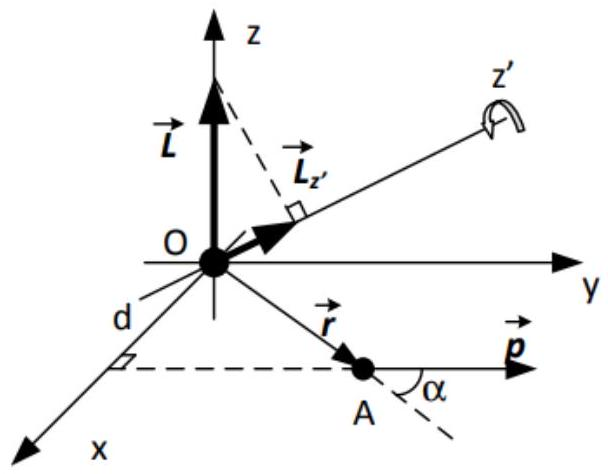
\includegraphics[width=0.5\textwidth]{2023_05_21_6e9b4e8657e82b213c6ag-03}
\end{figure}

Моментом импульса относительно оси z называется величина $\mathrm{L}_{\mathrm{z}}$, равная проекции на эту ось вектора момента импульса $\vec{L}$, определенного относительно произвольной точки O данной оси z. Значение момента импульса $\mathrm{L}_{\mathrm{z}}$ не зависит от положения точки $\mathrm{O}$ на оси z. При непрерывном распределении массы момент импульса относительно оси z равен:

$$
\overrightarrow{L_{z}}=J_{z} \overrightarrow{\omega_{z}}
$$

где $J_{z}$ - момент инерции тела относительно оси z, $\omega_{z}$ - угловая скорость вращения.

Момент импульса материальной точки или твердого тела связан с моментом приложенных сил следующим соотношением, называемым уравнением моментов:

$$
\frac{d \vec{L}}{d t}=\vec{M}
$$

Из уравнения моментов следует, что, если результирующий момент сил, действующий на систему материальных точек или твердое тело равен нулю (замкнутая система), то момент импульса такой системы остается постоянным:

$$
\vec{L}=\text { const }
$$

Если тело вращается вокруг закрепленной оси z, то сохраняется проекция момента импульса тела на эту ось:

$$
\overrightarrow{L_{z}}=\text { const }
$$

 \section{Теоремы об изменении количества движения материальной системы; об изменении главного момента количества движения материальной системы; об изменении кинетической энергии материальной системы.}


\begin{figure}[h!]
    \centering
    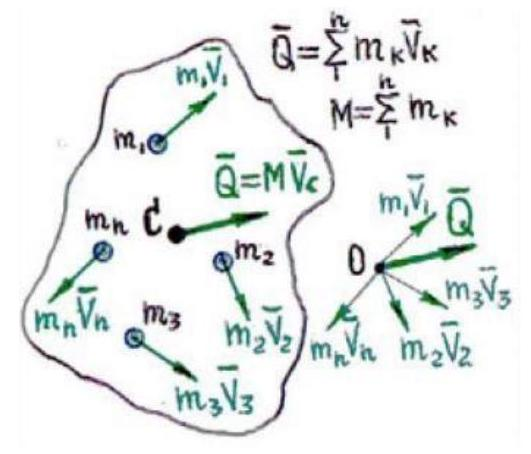
\includegraphics[width=0.5\textwidth]{2023_05_21_6e9b4e8657e82b213c6ag-05}
\end{figure}


\textbf{Теорема об изменении количества движения материальной системы:} Количество движения $\mathrm{mV}$ точки - произведение массы точки на вектор её скорости. Количеством движения системы - геометрическая сумма количеств движения всех её точек:

$$
\vec{Q}=\sum_{k=1}^{n} m_{k} \overrightarrow{v_{k}}
$$

Учитывая теорему о движении центра масс:

$$
M \vec{V}_{c}=\sum_{k=1}^{n} m_{k} \overrightarrow{v_{k}}
$$

Получаем, что:

$$
\vec{Q}=M \vec{V}_{c}
$$

Рассмотрим систему из $n$ материальных точек. Составим для этой системы дифференциальные уравнения движения и сложим их почленно:

$$
\frac{d \vec{Q}}{d t}=\frac{d}{d t} \sum_{k=1}^{n} m_{k} \overrightarrow{v_{k}}=\sum_{k=1}^{n} m_{k} \overrightarrow{a_{k}}=\sum_{k=1}^{n} \vec{F_{k}}^{\text{внутр}}+\sum_{k=1}^{n} \vec{F_{k}}^{\text{внешн}}
$$

С учетом того, что сумма внутренних сил 0 (3 закон Ньютона), то:

$$
\frac{d \vec{Q}}{d t}=\sum_{k=1}^{n} \\Vec{F_{k}}^{\text{внешн}}
$$

Тогда \textbf{теорема об изменении количества движения материальной системы:}

\begin{enumerate}
  \item В дифференциальной форме: производная по времени от количества движения системы равна геометрической сумме всех действующих на систему внешних сил.

  \item В интегральной форме: изменение количества движения системы за некоторый промежуток времени равно сумме импульсов, действующих на систему внешних сил за тот же промежуток времен.

\end{enumerate}

\textbf{Теорема об изменении главного момента количества движения материальной системы:}

Главный момент количества движения (кинетический момент) системы относительно данного центра $\mathrm{O}$ - величина $\mathrm{K}_{\mathrm{O}}$, равная геометрической сумме моментов количеств движения всех точек системы относительно этого центра:

$$
\overrightarrow{K_{O}}=\sum_{k=1}^{n} \overrightarrow{M_{0}}\left(m_{k} \overrightarrow{v_{k}}\right)=\sum_{k=1}^{n}\left[\overrightarrow{r_{k}} \times\left(m_{k} \overrightarrow{v_{k}}\right)\right]
$$

Рассмотрим одну материальную точку системы. Производная моментов количества движения равна (аддитивность сил и моментов):

$$
\frac{d}{d t} \overrightarrow{M_{0}}\left(m_{k} \overrightarrow{v_{k}}\right)=\overrightarrow{M_{0}}\left(\Vec{F_{k}}^{\text{внешн}}\right)+\overrightarrow{M_{0}}\left(\vec{F_{k}}^{\text{внутр}}\right)
$$

Где силы - равнодействующие внутренние и внешние составляющие, действующие на данную точку.

Тогда составляя данные уравнения для всех точек системы и складывая их почленно, получаем:

$$
\frac{d}{d t} \sum \overrightarrow{M_{0}}\left(m_{k} \overrightarrow{v_{k}}\right)=\sum \overrightarrow{M_{0}}\left(\Vec{F_{k}}^{\text{внешн}}\right)+\sum \overrightarrow{M_{0}}\left(\vec{F_{k}}^{\text{внутр}}\right)
$$

Но последняя сумма равно 0 (так как по 3 закону Ньютона сумма всех внутренних сил скомпенсируется, как и сумма моментов этих сил). Тогда:

$$
\frac{d \overrightarrow{\mathrm{K}_{\mathrm{o}}}}{d t}=\sum \overrightarrow{M_{0}}\left(\Vec{F_{k}}^{\text{внешн}}\right)
$$

Формулировка теоремы: производная по времени от главного момента количества движания системы относительно некоторого неподвижного центра равна сумме моментов всех внешних сил системы относительно того же центра.

$$
\vec{F}=m \frac{d \vec{v}}{d t}
$$

\textbf{Теорема об изменении кинетической энергии:}


1) Для материальной точки:


\begin{figure}[h!]
    \centering
    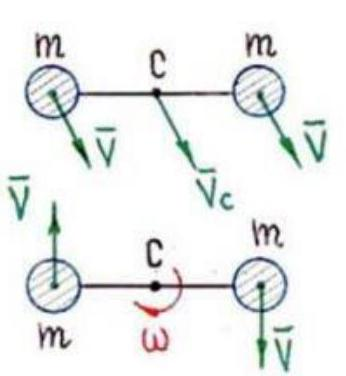
\includegraphics[width=0.4\textwidth]{2023_05_21_6e9b4e8657e82b213c6ag-06}
\end{figure}
Кинетическая энергия материальной точки - скалярная характеристика ее движения

$\mathrm{T}=\left(mv^{2} / 2\right)$.

В простейшей системе из двух равных по массе точек с поступательным движением $v$. Тогда очевидно, что

$$
T=\frac{m v^{2}}{2}+\frac{m v^{2}}{2}=m v^{2}
$$

Если вращательное движение с постоянной угловой скоростью $\omega$, то точки будут иметь одинаковые по величине скорости: $\mathrm{V}=\omega r$, тогда суммарная кинетическая энергия:

$$
T=\frac{m V^{2}}{2}+\frac{m V^{2}}{2}=m V^{2}
$$

То есть система обладает одинаковыми кинетическими энергиями, хотя движения разные. Кинетическая энергия не учитывает направленность движения.

Из второго закона Ньютона силу можно выразить как:

$$
\vec{F}=m \frac{d \vec{v}}{d t}
$$

Умножая скалярная данное произведение на dr получаем:

$$
\vec{F} d r=m \frac{d \vec{v}}{d t} d r=m \frac{d r}{d t} d \vec{v}=m v d \vec{v}=d\left(\frac{m v^{2}}{2}\right)=d A
$$

Это - математическая трактовка теоремы об элементарном изменении кинетической энергии точки: элементарное изменение кинетической энергии точки равно элементарной работе действующей на точку силы.

2)Для материальной системы:


Кинетической энергия системы называют скалярную величину $\mathrm{T}$, равную сумме кинетических энергий всех точек системы:

$$
T=\sum \frac{m v^{2}}{2}
$$

Доказанную выше теорему об элементарной изменении кинетической энергии точки применяем для всех точек системы и складываем почленно, получаем:

$$
d \sum\left(\frac{m v^{2}}{2}\right)=d T=\sum d A^{\text {внешних }}+\sum d A^{\text {внутренних }}
$$

Проинтегрировав обе части получаем:

$$
T_{1}-T_{0}=\sum A^{\text {внешних }}+\sum A^{\text {внутренних }}
$$

Это математическое представление теоремы об изменении кинетической энергии механической системы: изменение кинетической энергии системы на некотором её перемещении равно сумме работ всех внешних и внутренних сил, действующих на систему на этом перемещении.

\section{Относительное движение. Сложное движение. Силы инерции. Связи - идеальные, голономные, неголономные.}

Движение точки, рассматриваемое одновременно в неподвижной и подвижной систем отсчёта, называют сложным. При этом движение точки относительно неподвижной системы отсчёта называется абсолютным. Движение точки относительно подвижной системы отсчёта - относительное. Движение подвижной системы отсчета относительно неподвижной - переносное.



\begin{figure}[h!]
    \centering
    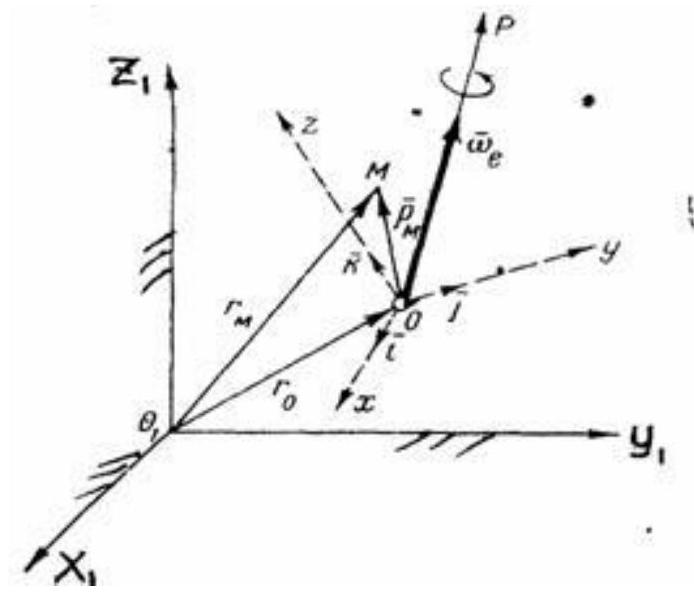
\includegraphics[width=0.5\textwidth]{2023_05_21_6e9b4e8657e82b213c6ag-07}
\end{figure}


$\mathrm{O}_{1} \mathrm{X}_{1} \mathrm{Y}_{1} \mathrm{Z}_{1}-$ неподвижная система координат. Вводится подвижная система координат OXYZ, совершающая заданное движение относительно неподвижной. Движение т.М относительно подвижной системы координат называется относительным. Траектории т.М относительно подвижной системы координат называется относительной. Скорость ОXYZ относительно $\mathrm{O}_{1} \mathrm{X}_{1} \mathrm{Y}_{1} \mathrm{Z}_{1}$ называется переменной. Скорость т.М относительно $\mathrm{O}_{1} \mathrm{X}_{1} \mathrm{Y}_{1} \mathrm{Z}_{1}$ называется абсолютной.

\textbf{Tеорема о сложении скоростей:} Вектор абсолютной скорости точки при сложном движении равен геометрической сумме её переносной и относительно скоростей:

$$
\bar{v}_{\text {абс }}=\bar{v}_{\text {пер }}+\bar{v}_{\text {отн }}
$$

\textbf{Теорема о сложении ускорений (Теорема Кориолиса):}


$$
\overrightarrow{\mathrm{a}_{\mathrm{aбc}}}=\overrightarrow{\mathrm{a}_{\text {отн }}}+\overrightarrow{\mathrm{a}_{\text {перен }}}+2 \overrightarrow{\boldsymbol{\omega}_{\text {перен }}} \times \overrightarrow{\boldsymbol{v}_{\text {отн }}}, \quad
\text{где } \overrightarrow{\mathrm{a}_{\text {кориолисово }}}=\mathbf{2} \overrightarrow{\boldsymbol{\omega}_{\text {перен }}} \times \overrightarrow{\boldsymbol{v}_{\text {отн }}}
$$


\begin{figure}[h!]
    \centering
    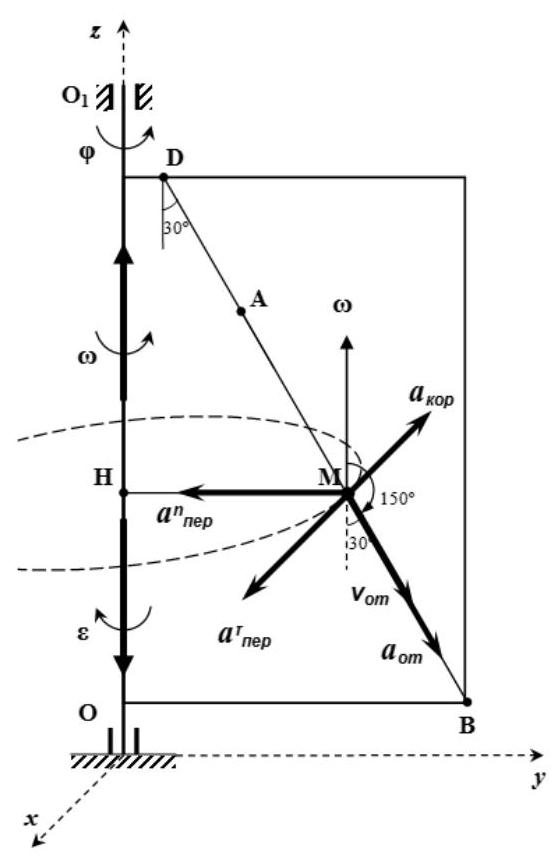
\includegraphics[width=0.5\textwidth]{2023_05_21_6e9b4e8657e82b213c6ag-08(1)}
\end{figure}


Кориолисово ускорение характеризует:

\begin{enumerate}
  \item Изменение модуля и направления переносной скорости точки из-за её относительности движения

  \item Изменение направления относительной скорости из- за вращательного переносного движения
\end{enumerate}

Направление кориолисова ускорения определяется по правилу Жуковского: 
Вектор относительной скорости спроецировать на плоскость, перпендикулярную переносной угловой скорости, и повернуть проекцию на $90^{\circ}$ в сторону вращения.

\textbf{Силы инерџии}


В общем случае сила инерции -векторная величина, равная произведению массы материальной точки на ее ускорение и направленная противоположно ускорению. Пусть F- активные силы, a R- силы реакции, тогда по второму закону Ньютона:

$$
m \overrightarrow{\mathrm{a}_{\mathrm{a} c}}=\sum \vec{F}+\vec{R}
$$

Раскрывая абсолютное ускорение по теореме Кориолиса:

$$
\begin{gathered}
m\left(\overrightarrow{\mathrm{a}_{\mathrm{oтн}}}+\overrightarrow{\mathrm{a}_{\text {перен }}}+\overrightarrow{\mathrm{a}_{\text {кориолиса }}}=\sum \vec{F}+\vec{R}\right. \\
m \overrightarrow{\mathrm{a}_{\mathrm{oтн}}}=\sum \vec{F}+\vec{R}-m \overrightarrow{\mathrm{a}_{\text {перен }}}-m \overrightarrow{\mathrm{a}_{\text {кориолиса }}} \\
m \overrightarrow{\mathrm{a}_{\mathrm{oтн}}}=\sum \vec{F}+\vec{R}+\overrightarrow{F_{\text {перен }}}+\overrightarrow{F_{\text {кориолиса }}}
\end{gathered}
$$
Тогда $\overrightarrow{F_{\text {перен }}=}-m \overrightarrow{\mathrm{a}_{\text {перен }}}-$ переносная сила инерции, 


$\overrightarrow{F_{\text {кориолиса }}}=-m \overrightarrow{\mathrm{a}_{\text {кориолиса) }}} $ кориолисова сила инерции.


\textbf{Связи}


Если на движение тела наложены некоторые ограничения, то говорят, что на движение тела нажжены связи. Связи - тела, ограничивающие свободу перемещения данной точки или тела, наложенным на данную точку или тело.

Идеальные связи: в которых отсутствует трение. При этом сумма элементарных работ реакций связей на элементарных перемещениях равна нулю.

Основные виды идеальных связей:

\begin{figure}[h!]
    \centering
    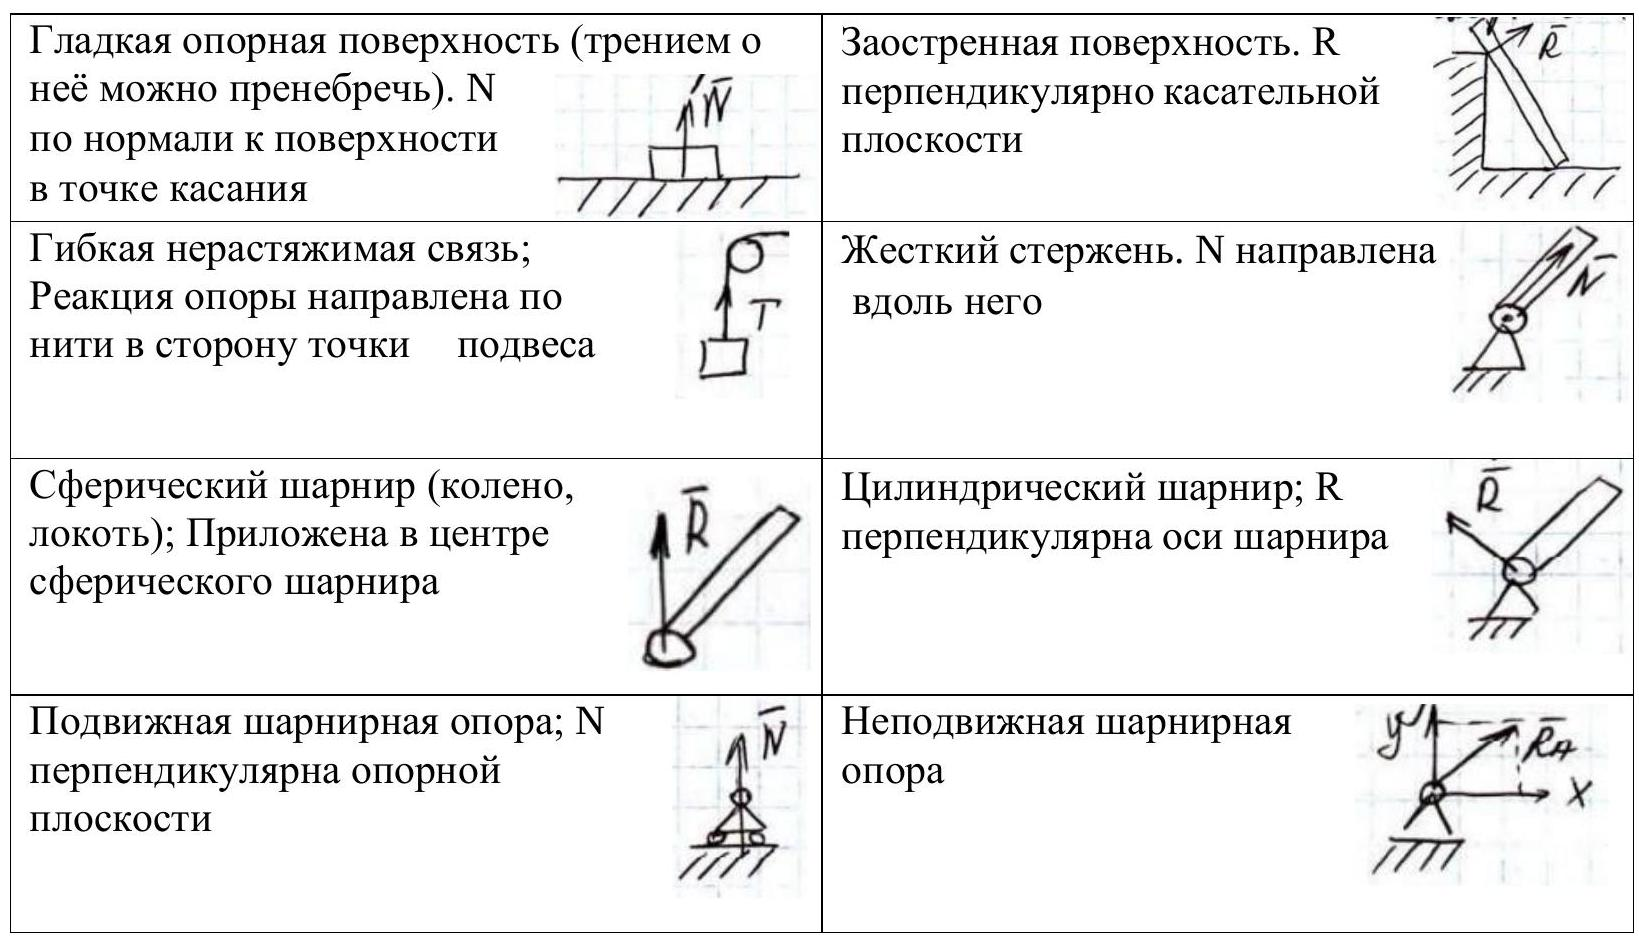
\includegraphics[width=1\textwidth]{2023_05_21_6e9b4e8657e82b213c6ag-09}
\end{figure}


Связи, налагающие ограничения на положения точек системы - геометрические, а налагающие ограничения еще и на скорости- кинематические (дифференциальньими). Геометрические и интегрируемые дифференциальные связи называют связями голономными, а неинтегрируемые дифференциальные связи - неголономными. По виду связей механические системы тоже разделяют на голономные (с голономными связями) и неголономныlе (содержащие неголономные связи).

\section{Уравнения Лагранжа второго рода.}
Общее уравнение динамики:
Рассмотрим систему материальных точек, на которую наложены стационарные, идеальные, голономные связи. Тогда \textbf{принцип возможных перемещений}: При равновесии материальной системы с идеальными и стационарными связями сумма работ всех активных, задаваемых, сил на любом возможном перемещении системы из положения равновесия равна нулю:

$$
\sum_{k=1}^{n} \overrightarrow{F_{k}^{\text{акт}}} \delta \overrightarrow{r_{k}}=\sum_{k=1}^{n} \delta A_{k}^{\text{акт}}=0
$$

Принцип Даламбера позволяетрассматривать динамическую систему как статическую, если к ней добавить силы инерции:

$$
\sum_{k=1}^{n} \delta A_{k}^{\text {акт }}+\sum_{k=1}^{n} \delta A_{k}^{\text {инерц }}=0
$$
Это общее уравнение динамики.


\textbf{Обобщенные координаты:} Положение механической системы, состоящей из $\mathrm{n}$ материальных точек определяется $3 \mathrm{n}$ декартовыми координатами: $x_1, y_1, x_1, ..., x_n, y_n, z_n.$. Пусть на систему наложено $l$ геометрических удерживающих связей. Связи накладывают ограничения на декартовы координаты, записываемые в виде соотношений: $f k(x_1, y_1, z_1, \ldots$, $x_n, y_n, z_n)=0$ гдe $k=1 \ldots l$ - уравнения связей. Из уравнения связей определяют $Зn-l=s$ координат, все декартовы координаты однозначно выражают через $s$ каких-либо независимых параметров $q_1, q_2, \ldots, q_s$, которые называются обобщенными координатами. 

Обобщенные координаты - любые независимые параметры, которые полностью и однозначно определяют положение системы. Тогда в обобщенных координатах общее уравнение динамики может быть записано через частные производные:

Где $\mathrm{Q}_{\mathrm{i}}$ - обобщенные силы:

$$
\sum_{i=1}^{s}\left(Q_{i}^{\text {акт }}+Q_{i}^{\text {инерц }}\right) \delta q_{i}=0
$$

$$
\left\{\begin{array}{c}
Q_{i}^{\text {акт }}=\sum_{k=1}^{n} \overrightarrow{F_{k}^{\text {акт }}} \frac{\delta \overrightarrow{r_{k}}}{\delta q_{i}}-\text { активная часть } \\
Q_{i}^{\text {инерц }}=\sum_{k=1}^{n} \overrightarrow{F_{k}^{\text {инерц }}} \frac{\delta \overrightarrow{r_{k}}}{\delta q_{i}}-\text { инерциальная часть }
\end{array}\right.
$$

Раскрывая обобщенные силы и инерциальную силу расписывая как произведение массы и соответствующего ускорения:

$$
\sum_{i=1}^{s}\left[\sum_{k=1}^{n} m_{k} \frac{d \overrightarrow{V_{k}}}{d t} \frac{d \overrightarrow{r_{k}}}{d q_{i}}-\sum_{k=1}^{n} \overrightarrow{F_{k}^{\text{акт}}}\right] \delta q_{i}=0
$$

Рассмотрим преобразования первого слагаемого:

$$\sum_{k=1}^{n} m_{k} \frac{d \overrightarrow{V_{k}}}{d t} \frac{d \overrightarrow{r_{k}}}{d q_{i}}=\frac{d}{d t}\left(\frac{d T}{d \dot{q}_{l}}\right)-\frac{d T}{d q_{i}}$$

Подставим это выражение в сумму:

$$
\sum_{i=1}^{s}\left[\frac{d}{d t}\left(\frac{d T}{d \dot{q}_{l}}\right)-\frac{d T}{d q_{i}}-Q_{i}^{\text{акт}}\right]=0
$$

Обобщенные координаты независимы, поэтому сумма может обратиться в 0, только когда каждое из слагаемых будет 0. Тогда уравнение Лагранжа 2 рода (уравнение движения механической системы в обобщенных координатах):

$$
\frac{d}{d t}\left(\frac{d T}{d \dot{q}_{l}}\right)-\frac{d T}{d q_{i}}=Q_{i}^{\text {акт }}
$$

Число таких уравнений соответствует числу степеней свободы s.


Преимущество этих уравнений, что их вид и число не зависит на прямую от количества точек, входящих в систему. Также данные уравнения инварианты относительно того, как эти тела (точки) движутся.


\section{Уравнения баланса массы, импульса, момента импульса, энергии в механике сплошной среды. Понятие о замкнутой системе уравнений.}
Закон сохранения массы: Пусть V - неподвижный объем, из которого вытекает или втекает вещество. Масса внутри объема будет вычисляться по формуле $m=\int_{V} \rho d V$

Тогда для изменения массы запишем:

$$
\frac{\partial m}{\partial t}=\frac{\partial}{\partial t} \int_{V} \rho d V=\int_{V} \frac{\partial \rho}{\partial t} d V+\int_{\Sigma} \rho v_{n} d S=0
$$

Где $V_n$ - скорость потока по нормали к поверхности $\mathrm{S}$ объема $\mathrm{V}, \Sigma$ - граница объема $\mathrm{V}$. Второе слагаемое в правой части равенства выражает поток через границу объема, а первый член характеризует изменение плотности внутри V. Далее используя теорему Остроградского- Гаусса:

$$
\int_{S} v_{n} d S=\int_{V} \mathrm{div} \vec{v} d V
$$

Получаем \textbf{закон сохранения массы:}

$$
\frac{\partial \rho}{\partial t}+\mathrm{div}(\rho \vec{v})=\frac{\partial \rho}{\partial t}+\rho \mathrm{div}(\vec{v})=0
$$

Если жидкость несжимаема, то ее плотность постоянна, $\rho=$ const, следовательно, $\frac{\partial \rho}{\partial t}=0$ и плотность можно вынести из-под оператора дивергенции и сократить. Получим $\mathrm{div}(\vec{v})=0$

\textbf{Закон сохранения импульса:} Возьмем тот же объем, импульс объема определяется выражением $\boldsymbol{q}=\int_{V} \rho \mathbf{v} d V$. Тогда в интегральной форме уравнение сохранения импульса запишется как:

$$
\frac{\partial q}{\partial t}=\frac{\partial}{\partial t} \int_{V} \rho v d V=\int_{V} \rho F d V-\int_{\Sigma} \rho v v_{n} d S+\int_{\Sigma} P_{n} d S
$$

Где левая часть - изменение импульса объема, первое слагаемое в правой части импульс втекающего вещества. $\mathbf{P}$ - тензор напряжений $\mathrm{p}_{\mathrm{ij}} \mathbf{p}_\mathbf{n}=\mathrm{P}_{\mathrm{ij}}\left(\mathrm{n}_{1} \mathrm{n}_{2} \mathrm{n}_{3}\right)^{\mathrm{T}},\quad\left(\mathrm{p}_{\mathrm{n}}\right)_{\mathrm{i}}=\sum\mathrm{P}_{\mathrm{i j}} \mathrm{n}_{\mathrm{j}}$

Применим теорему Гаусса-Остроградского:

$$
\frac{\partial}{\partial t} \int_{V} \rho v d V=\int_{V} \rho F d V-\Sigma \int_{\mathrm{V}} \nabla_{k}\left(\rho v_{i} v_{n}\right) e_{i} d S+\Sigma \int_{\mathrm{v}} \nabla_{k} P_{i k} d V e_{i}
$$

Тогда баланс импульса примет вид (приравниваем к 0), а интеграл общий, значит подынтегральные выражения должны быть в сумме 0:

где $\mathrm{i}=1,2,3$

$$
\frac{\partial}{\partial t}\left(\rho v_{i}\right)+\frac{\partial}{\partial x^{k}}\left(\rho v_{i} v_{k}\right)=\frac{\partial}{\partial x^{k}} P_{i k}+\rho F_{i}
$$

Раскрывая и применяя закон сохранения массы:

$$
\rho a_{i}=\frac{\partial}{\partial x^{k}} P_{i k}+\rho F_{i}
$$

Где $a_{i}$ ускорение.

\textbf{Баланс момента импульса:}
Момент импульса можно представить как векторное произведение: $\boldsymbol{q}=\int_{V}[r \times \rho v] d V$. Тогда

$$
\frac{\partial}{\partial t} \int_{V}[r \times \rho v] d V=\int_{V}[r \times \rho F] d V-\int_{\Sigma}[r \times \rho v] v_{n} d S+\int_{\Sigma}\left[r \times P_{n}\right] d S
$$

\begin{enumerate}
  \item У среды нет собственного момента импульса при $\mathrm{v} \equiv 0$

  \item Нет внешних объемных поверхностных моментов

\end{enumerate}

Из уравнения баланса момента импульса в классическом случае следует симметричность тензора напряжений: $P_{i j}=P_{j i}$

\textbf{Закон сохранения энергии:}
Пусть дан объем жидкости $\mathrm{V}$, тогда в интегральном виде изменение энергии можно записать в виде:

$$
\frac{\partial}{\partial t} \int_{V} \rho\left(\varepsilon+\frac{v^{2}}{2}\right) d V=\int_{V} j \cdot f d V+\int_{\Sigma} a \cdot n d S-\int_{\Sigma} q \cdot n d S+\int_{V} r \cdot p d V
$$

Где $\varepsilon$ -- массовая плотность внутренних энергий, q-вектор плотности потока тепла, а -- вектор плотности потока энергия, связанный с работой внутренних напряжений, r -- объемная плотность внешних источников энергии, f -- вектор массовой плотности внешних сил, ј --поток массы, p тензор напряжений, $\mathrm{n}$ -- вектор нормали. 


В результате первое слагаемое -- работа внешних сил, второе -- работа напряжений, третье -- тепловой поток, четвертое -- энергия от внешних источников.

Применим аналогичные предыдущим действия (теорема Гаусса-Остроградского + упростим до полной производной) и получим дифференциальную форму:

$$
\frac{\partial\left(\rho\left(\varepsilon+\frac{v^{2}}{2}\right)\right)}{\partial t}+\mathrm{div}\left(\varepsilon+\frac{v^{2}}{2}\right) v_{i}=j \cdot f+\mathrm{diva}-\mathrm{divq}+r \cdot p
$$

Недивергентные слагаемые соответствуют работе внешних сил и внешним источникам тепла

\textbf{Понятие о замкнутой системе уравнений:} В гидромеханической задаче всегда даны связи:

\begin{enumerate}
  \item Баланс массы
  \item Баланс импульса;
  \item Баланс момента импульса
\end{enumerate}

Если неизвестных меньше чем уравнений, система называется замкнутой.

Неизвестные: $\rho=\rho(\mathrm{x}, \mathrm{y}, \mathrm{z}, \mathrm{t}), \quad \mathrm{v}=\mathrm{v}(\mathrm{x}, \mathrm{y}, \mathrm{z}, \mathrm{t}), \quad \mathrm{P}_{\mathrm{ij}}=\mathrm{P}_{\mathrm{ij}}(\mathrm{x}, \mathrm{y}, \mathrm{z}, \mathrm{t})$

Часто задан $\mathrm{F}$, например $\mathrm{F}=\mathrm{g}$ (сила тяжести)

\section{Модель идеальной жидкости. Уравнения Эйлера. Полная система уравнений. Типичные граничные условия.}
\textbf{Модель идеальной жидкости} --- простейшая модель движущейся жидкости. Не учитывает наличие внутреннего трения (вязкости). По площадкам соприкосновения двух объемов действуют только нормальные к площадкам напряжения, касательных нет.

Модель идеальной жидкости применяется для изучения течения с большими скоростями, кавитационных течений, течений со свободными границами. В рамках данной модели считается, что нет потерь механической энергии.

В идеальной жидкости тензор напряжений имеет вид:

$$
p_{i j}=-p E_{n}=\left(\begin{array}{ccc}
-p & 0 & 0 \\
0 & -p & 0 \\
0 & 0 & -p
\end{array} \right)
$$

\begin{enumerate}
  \item Уравнение движения идеальной жидкости (Уравнение Эйлера):
\end{enumerate}
$$
\rho\left(\frac{\partial \vec{v}}{\partial t}+(\vec{v} \nabla) \vec{v}\right)=-\mathrm{grad} p+\rho \vec{f}
$$

Где $v$ - скорость потока, f-вектор массовой плотности внешних сил.

В проекции на координатные оси:

$$
\left\{\begin{array}{l}
Ox: \rho\left(\frac{\partial \overrightarrow{v_{x}}}{\partial t}+v_{x} \frac{\partial \overrightarrow{v_{x}}}{\partial x}+v_{y} \frac{\partial \overrightarrow{v_{y}}}{\partial x}+v_{z} \frac{\partial \overrightarrow{v_{z}}}{\partial x}\right)=-\frac{\partial p}{\partial x}+\rho f_{x} \\
Oy: \rho\left(\frac{\partial \overrightarrow{v_{y}}}{\partial t}+v_{x} \frac{\partial \overrightarrow{v_{x}}}{\partial x}+v_{y} \frac{\partial \overrightarrow{v_{y}}}{\partial x}+v_{z} \frac{\partial \overrightarrow{v_{z}}}{\partial x}\right)=-\frac{\partial p}{\partial y}+\rho f_{y} \\
Oz: \rho\left(\frac{\partial \overrightarrow{v_{z}}}{\partial t}+v_{x} \frac{\partial \overrightarrow{v_{x}}}{\partial x}+v_{y} \frac{\partial \overrightarrow{v_{y}}}{\partial x}+v_{z} \frac{\partial \overrightarrow{v_{z}}}{\partial x}\right)=-\frac{\partial p}{\partial z}+\rho f_{z}
\end{array}\right.
$$

\begin{enumerate}
  \setcounter{enumi}{1}
  \item Закон сохранения массы:
\end{enumerate}

$$
\frac{\partial \rho}{\partial t}+\mathrm{div}(\rho \vec{v})=\frac{\partial \rho}{\partial t}+\rho \mathrm{div}(\vec{v})=0
$$

Если жидкость несжимаемая, то есть $\rho=$ const, то $\mathrm{div}(\vec{v})=0$.

\begin{enumerate}
  \setcounter{enumi}{2}
  \item Уравнения состояния: $p=p(\rho)$ или $\rho=\rho(p)$
\end{enumerate}

Система уравнений 1), 2), 3) при заданных начальных и граничных условиях называется полной системой уравнений. Начальные условия: параметры в момент времени $\mathrm{t}=0: V_0, р_0 и \rho_{0}$.

Типичные граничные условия:

\begin{enumerate}
  \item Граница «жидкость-твердое» (стенка):
\end{enumerate}


\begin{figure}[h!]
    \centering
    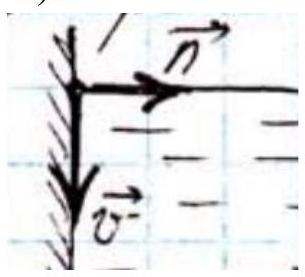
\includegraphics[width=0.2\textwidth]{2023_05_21_6e9b4e8657e82b213c6ag-13}
\end{figure}


a) если стенка неподвижна, то условие непротекания:
$
\left.\vec{v} \cdot \vec{r}\right|_{\text {граница }}=0
$

б) если стенка движется:
$
\left.\vec{v} \cdot \vec{r}\right|_{\text {граница }}=D
$
где D -скорость движения стенки по нормали к ней.

\begin{enumerate}
  \setcounter{enumi}{1}
  \item Граница «жидкость-воздух»
\end{enumerate}

а) если пренебречь атмосферным давлением:
$
\left.\vec{v} \cdot \vec{r}\right|_{\text {граница }}=0
$


б) $\left.\mathrm{p}\right|_{\Gamma}=p_{\text {aтм }}-$ если пренебречь капиллярными эффектами


в) $\left.\mathrm{p}\right|_{\Gamma}-\mathrm{p}_{\text {атм }}=\sigma\left(1 / \mathrm{R}_1-1 / \mathrm{R}_2\right)-$ с учетом капиллярных давлений


\section{Идеальная жидкость. Уравнения Эйлера в форме Громеки- Лэмба. Интеграл Бернулли. Интеграл Коши-Лагранжа. Примеры.}

\textbf{Модель идеальной жидкости} - простейшая модель движущейся жидкости. Не учитывает наличие внутреннего трения (вязкости). По площадкам соприкосновения двух объемов действуют только нормальные к площадкам напряжения, касательных нет.

Модель идеальной жидкости применяется для изучения течения с большими скоростями, кавитационных течений, течений со свободными границами. В рамках данной модели считается, что нет потерь механической энергии.

В идеальной жидкости тензор напряжений имеет вид:

$$
p_{i j}=-p E_{n}=\left(\begin{array}{ccc} 
-p & 0 & 0 \\
0 & -p & 0 \\
0 & 0 & -p
\end{array} \right)
$$

Уравнение движения идеальной жидкости (Уравнение Эйлера):

$$
\rho\left(\frac{\partial \vec{v}}{\partial t}+(\vec{v} \nabla) \vec{v}\right)=-\mathrm{gradp}+\rho \vec{f}
$$

Где $v$ - скорость потока, f-вектор массовой плотности внешних сил.

Если левую часть переписать в виде:

$$
\frac{\partial \vec{v}}{\partial t}+(\vec{v} \nabla) \vec{v}=\frac{\partial \vec{v}}{\partial t}+\mathrm{grad} \frac{v^{2}}{2}+[\mathrm{rot} \vec{v} \times \vec{v}]
$$

Получится \textbf{уравнение Эйлера в форме Громеки-Лэмба:}

$$
\rho\left(\frac{\partial \vec{v}}{\partial t}+\mathrm{grad} \frac{v^{2}}{2}+[\mathrm{rot} \vec{v} \times \vec{v}]\right)=-\mathrm{gradp}+\rho \vec{f}
$$

Данная форма записи позволяет получить вывод интеграла Бернули:

\begin{enumerate}
  \item Считаем жидкость идеальной

  \item Течение стационарно, т.е. $\frac{\partial \mathbf{v}}{\partial t}=0$

  \item Жидкость несжимаема $\rho=$ const

  \item Объемные силы потенциальны, т.е. $\mathbf{F}=\mathrm{grad}(\mathbf{u})$ (u-потенциальное поле энергий)

  \item Будем рассматривать проекции на линии тока, которая совпадает с траекторией

\end{enumerate}


\begin{figure}[h!]
    \centering
    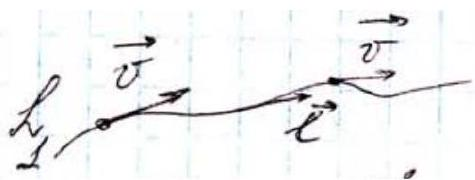
\includegraphics[width=0.5\textwidth]{2023_05_21_6e9b4e8657e82b213c6ag-14(2)}
\end{figure}

Домножим уравнение Эйлера в форме Громеки-Лэмба на $l$ - вектор касательной к линии тока. Тогда:

$$
\begin{gathered}
\rho\left(\mathrm{grad} \frac{v^{2}}{2}+[\mathrm{rot} \vec{v} \times \vec{v}]\right)=-\mathrm{grad} p+\rho \vec{f} \mid \cdot \vec{l} \\
\rho\left(\left(\mathrm{grad} \frac{v^{2}}{2}\right) \cdot \vec{l}+([\mathrm{rot} \vec{v} \times \vec{v}]) \cdot \vec{l}\right)=-\mathrm{grad} p\cdot \vec{l}+\rho \vec{f} \cdot \vec{l} \\
([\mathrm{rot} \vec{v} \times \vec{v}]) \cdot \vec{l})=0 \text { так как векторы ортонормальны } \\
\vec{f}=\mathrm{grad}(u)
\end{gathered}
$$

Получаем уравнение:

$$
\mathrm{grad}\left(\rho \frac{v^{2}}{2}+p-\rho u\right) \cdot \vec{l}=0
$$

$\Gamma$ радиент $=0$, если:

$\rho \frac{v^{2}}{2}+p-\rho u=$ const вдоль линий тока

\textbf{Этот закон называется интегралом Бернулли}


Примеры:


a) Стачионарное течение жидости из сосуда
\begin{figure}[h!]
    \centering
    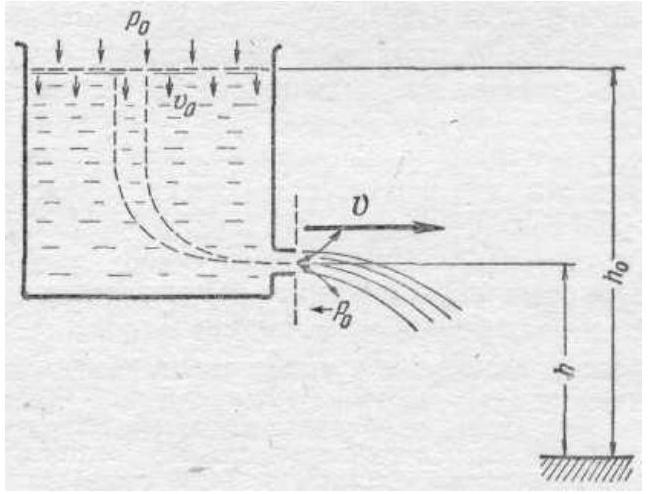
\includegraphics[width=0.5\textwidth]{2023_05_21_6e9b4e8657e82b213c6ag-15}
\end{figure}


Сверху: $\mathrm{p}=\mathrm{p}_{\text {атм }}, \vec{v} \approx 0$ так как сосуд достаточно большой, $\mathrm{z}=\mathrm{h}_{0}$

В дырке на дне: $\mathrm{p}=\mathrm{p}_{\text {атм }}, \mathrm{z}=\mathrm{h}$

Задача состоит в нахождении скорости вытекания воды $\mathrm{v}$

Пусть $\mathrm{H}=\mathrm{h}_{\mathrm{o}}-\mathrm{h}$

Тогда запишем уравнение Бернулли для точки сверху и для точки в дырке на дне (они будут равны, так как уравнение Бернулли должно быть постоянным):

Сверху: $p_{\text {атм }}+\rho g h_{0}$

В дырке: $\rho \frac{v^{2}}{2}+p_{\text {атм }}+\rho g h$

Приравниваем: $\rho \frac{v^{2}}{2}+p_{\text {атм }}+\rho g h=p_{\text {атм }}+\rho g h_{0}$

Тогда: $\rho \frac{v^{2}}{2}=\rho g H$

Выражая скорость из данного уравнения, получаем формулу Торричелли:

$$
v=\sqrt{2 g H}
$$

б) Работа трубки Пито - Прандтля: аэродинамический прибор для измерения динамического давления.

\begin{figure}[h!]
    \centering
    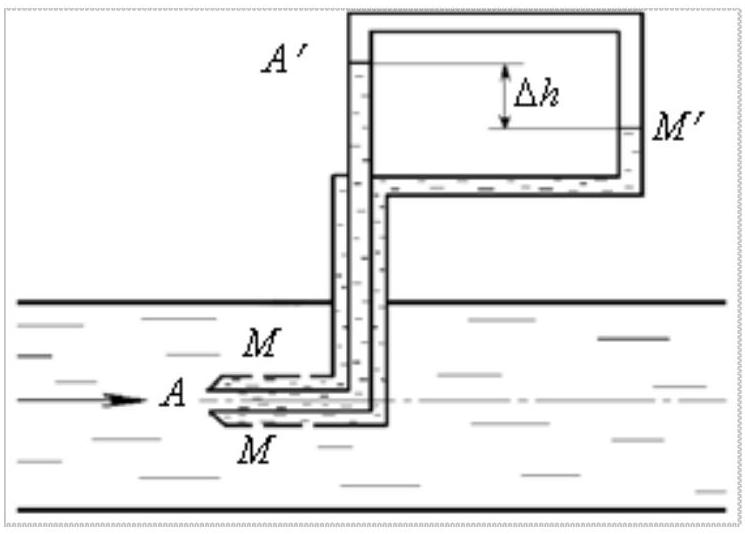
\includegraphics[width=0.5\textwidth]{2023_05_21_6e9b4e8657e82b213c6ag-16(1)}
\end{figure}

Через отверстие А происходит измерение динамического давления. Через отверстия М измеряется статическое давление жидкости.

Записываем уравнение Бернулли для точек А и М:

$$
p_{M}=p_{A}+\rho \frac{v^{2}}{2}
$$

Тогда скорость потока жидкости:

$$
v=\sqrt{\frac{2\left(p_{M}-p_{A}\right)}{\rho}}
$$

Применим для идеальной жидкости в случае потенциальньх течений: $\rho=\mathrm{const}, \vec{v}=\mathrm{grad} \varphi, \vec{f}=$ $\mathrm{grad} \Phi$, где $\Phi$ - потенциал массовых сил, $\phi$ - потенциал скорости. Тогда применим уравнение Эйлера в форме Громеки-Лэмба:
$$
\rho\left(\frac{\partial \vec{v}}{\partial t}+\mathrm{grad} \frac{v^2}{2}+[\mathrm{rot} \vec{v} \times \vec{v}]\right)=-\mathrm{grad} p+\rho \vec{f}
$$
С учетом того, что для потенциального поря rot $=0$, то
$$
\rho\left(\frac{\partial \overrightarrow{\nabla \varphi}}{\partial t}+\mathrm{grad} \frac{(\overrightarrow{\nabla \varphi})^2}{2}+[\mathrm{rot} \vec{v} \times \vec{v}]\right)=-\vec{\nabla} p+\rho \overrightarrow{\nabla \Phi}
$$
Тогда получаем:
$$
\mathrm{grad}\left(\frac{\partial \varphi}{\partial t}+\frac{(\nabla \varphi)^2}{2}+\frac{p}{\rho}-\Phi\right)=0
$$
Градиент будет равен нулю только если выражение в скобках будет константой:
$$
\frac{\partial \varphi}{\partial t}+\frac{(\nabla \varphi)^2}{2}+\frac{p}{\rho}-\Phi=\mathrm{const}
$$
 \textbf{интеграл Коши-Лагранжа}, выполняется во всей жидкости. Константа зависит только от времени.

 
Пример: Жидкость в поле сильы тяжести.

\section{Модель линейно-вязкой несжимаемой жидкости. Уравнения Навье-Стокса. Полная система уравнений. Условие прилипания на границе с твердым телом. Понятие о ламинарном и турбулентном режимах течения.}


В отличие от невязкой идеальной жидкости, в вязкой присутствует внутреннее трение (вязкость), которое приводит к диссипации энергии. Согласно Ньютону: касательные напряжения трения в прямолинейнодвижущейся вязкой жидкости пропорционально изменению скорости по нормали к направлению движения жидкости:
\begin{figure}[h!]
    \centering
    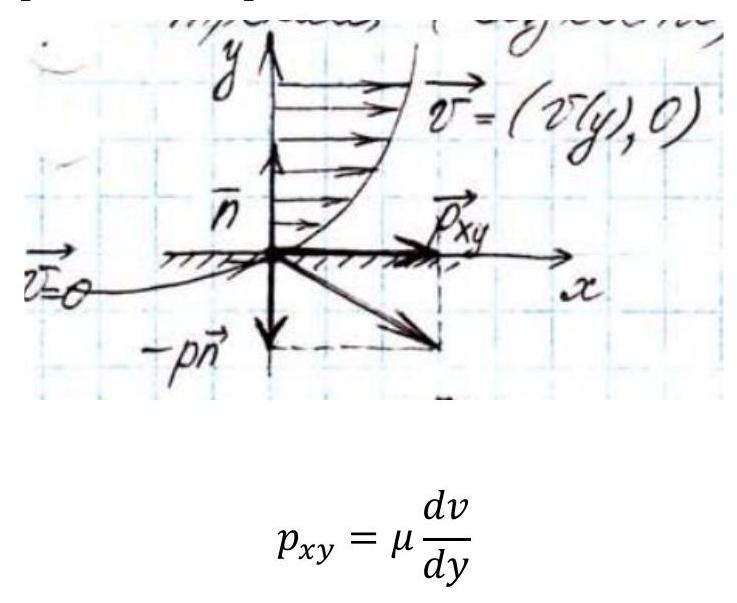
\includegraphics[width=0.5\textwidth]{2023_05_21_6e9b4e8657e82b213c6ag-17}
\end{figure}
где $\mu-$ коэффициент вязкости

В вязкой жидкости тензор напряжений имеет вид: $\boldsymbol{p}_{i j}=-p \delta_{i j}+\tau_{i j}$, где $\boldsymbol{\delta}_{i j}-$ символ Кронекера, $\tau_{i j}-$ тензор вязких напряжений. В несжимаемой жидкости: $\tau_{i j}=2 \mu e_{i j}$

\textbf{Закон Навье-Стокса для несжимаемой жидкости:}
$$
\begin{aligned}
& p_{i j}=-p \delta_{i j}+2 \mu e_{i j} \\
& e_{i j}=\frac{1}{2}\left(\frac{\partial v_{i}}{\partial x_{j}}+\frac{\partial v_{j}}{\partial x_{i}}\right)
\end{aligned}
$$

Тогда тензор напряжений можно записать:

$$
\left(p_{i j}\right)=\left(\begin{array}{cc}
-p & 0 \\
0 & -p
\end{array}\right)+\left(\begin{array}{cc}
0 & \mu \frac{d v}{d y} \\
\mu \frac{d v}{d y} & 0
\end{array}\right)=\left(\begin{array}{cc}
-p & \mu \frac{d v}{d y} \\
\mu \frac{d v}{d y} & -p
\end{array}\right)
$$

\begin{enumerate}
  \item Закон сохранения массы для несжимаемой жидкости: $\mathrm{div} v=0$
  \item Уравнение движения жидкости (уравнение Эйлера):
\end{enumerate}

$$
\rho\left(\frac{\partial \vec{v}}{\partial t}+(\vec{v} \nabla) \vec{v}\right)=-\mathrm{gradp}+\rho \vec{f}
$$

Где тензор напряжений

$$
p_{i j}=-p \delta_{i j}+2 \mu e_{i j}=-p \delta_{i j}+\mu \mathrm{grad} vec{v}
$$

Тогда уравнение движения примет вид (\textbf{это уравнение Навье-Стокса}):

$$
\rho\left(\frac{\partial \vec{v}}{\partial t}+(\vec{v} \nabla) \vec{v}\right)=-\mathrm{grad} p+\mu \Delta \vec{v}+\rho \vec{f}
$$

Где $\Delta$ - оператор Лапласа.


Система уравнений 1 и 2 с заданными граничными условиями - полная система уравнений.

\textbf{Граничные условия:}


a) Жидкость-твердое (стенка):
$\left.\mathbf{v}\right|_{\Gamma}=\mathbf{D}-$ где $\mathrm{D}$ скорость стенки

(В частном случае, для неподвижной стенки $\left.\mathbf{v}\right|_{\Gamma}=\mathbf{0}$ - \textbf{условие прилипания})

б) Граница между двумя вязкими жидкостями:

\begin{enumerate}
  \item $\left.\mathbf{v}_2\right|_{\Gamma}=\left.\mathbf{v}_1\right|_{\Gamma}-$ равенство скоростей

  \item $\left.\left(\mathrm{p}^{1}{ }_{\mathrm{ij}}-\mathrm{p}^{2} _\mathrm{ij}\right)\right|_{г} \mathrm{n}_{\mathrm{j}}=0$ равенство действующих друг на друга сил

\end{enumerate}

\textbf{Ламинарное и турбулентное движение жидкости:}

\begin{figure}[h!]
    \centering
    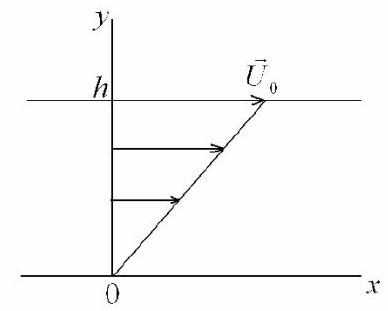
\includegraphics[width=0.5\textwidth]{2023_05_21_6e9b4e8657e82b213c6ag-18}
\end{figure}


Ламинарное движение - плоскопараллельное, когда линии тока - прямые линии. Это выполняется когда скорость направлена только по оси $\mathrm{x}$, а составляющая по у $\mathrm{V}_{\mathrm{y}}=0$.

Пример - движение жидкости между параллельными неподвижными пластинами:
\begin{figure}[h!]
    \centering
    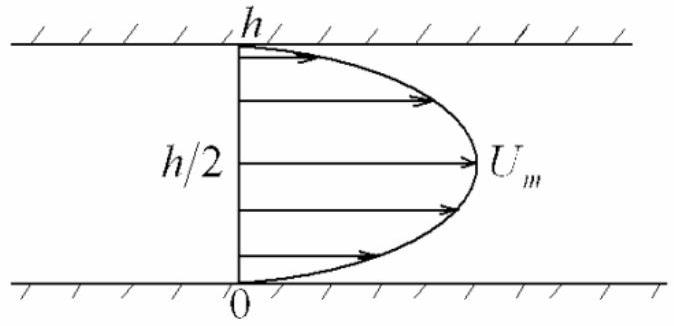
\includegraphics[width=0.5\textwidth]{2023_05_21_6e9b4e8657e82b213c6ag-18(1)}
\end{figure}

Турбулентное - возмущенное, неустойчивое течение жидкости. Характеристикой, которая разграничивает эти режимы течения, является число Рейнольдса.

\textbf{Число Рейнольдса} - безразмерная величина, характеризующая отношение силы инерции к силе трения:

$$
R e=\frac{\rho v^{2}}{l}: \frac{\mu v}{l^{2}}=\frac{\rho v l}{\mu}
$$

Где v - средняя скорость движения (характерная скорость), l - характерная длина (размер тела или ширина канала), $\rho$ - плотность жидкости. $\mu$ - вязкость.

При $\mathrm{Re}<\mathrm{Re}_{\text {кр }}$ наблюдается упорядоченное ламинарное течение.

При $\mathrm{Re}>\mathrm{Re}_{\text {кр }}-$ течение турбулентное, хаотическое.

\section{Определяюшие параметры явления. Класс систем единиц. Размерность физической величины. П-теорема теории размерностей. Моделирование физических процессов на основе П-теоремы. Критерии подобия. Примеры (число Рейнольдса).}
\textbf{Физические величины:}
\begin{enumerate}
  \item Первичные (основные) величины: L - единица длины; $\mathrm{M}$ - единица массы; $\mathrm{T}$ единица времени. Образуют класс $\{\mathrm{LMT}\}$. Пример: международная система СИ и СГС.

  \item Вторичные (производные) величины: $\rho, \mathrm{v}, \mathrm{F}$ и тд

\end{enumerate}

Цель физического исследования --- поиск связи между численными значениями искомого параметра а и численными значениями других параметров $a_{1}, a_{2}, a_{3} \ldots a_{n}$ от которых он зависит. а --- определяемый параметр. $\mathrm{a}_{1}, \mathrm{a}_{2}, \mathrm{a}_{3} \ldots \mathrm{a}_{\mathrm{n}}$ - определяющие параметры.

$$
a=f\left(a_{1}, a_{2}, a_{3} \ldots a_{n}\right)
$$

Пусть определяемый и определяющие параметры измеряются в системе LMT. Тогда размерность каждой величины представляется в виде:

$$
\begin{gathered}
\mathrm{dim} a=[a]=L^{\alpha} M^{\beta} T^{\gamma} \\
\mathrm{dim} a_{i}=\left[a_{i}\right]=L^{\alpha i} M^{\beta i} T^{\gamma i}
\end{gathered}
$$

Если $\alpha, \beta, \gamma=0$ то такая физическая величина безразмерна.

\underline{Определение 1.} Параметры $\mathrm{a}_{1}, \mathrm{a}_{2}, \mathrm{a}_{3} \ldots \mathrm{a}_{\mathrm{n}}$ размерно независимыь, если из них можно составитьтолько тривиальную безразмерную комбинацию, т.е.:

$$
\left[\mathrm{a}_{1}{ }^{\mathrm{k}_1} \mathrm{a}_{2}{ }^{\mathrm{k}_2} \mathrm{a}_{3}{ }^{\mathrm{k}_3} \ldots \mathrm{a}_{\mathrm{n}}^{\mathrm{k_n}}\right]=1 \text {, если для всех } \mathrm{ki}=0 \text {, для любых } \mathrm{i}
$$

Пример: $\mathrm{v}- \text{м/c}, \rho-\text{кг/м3} $ --- размерно независимы

$\mathrm{v}-\text{м/c}, \quad \rho-\text{кг/м3}, \quad\mathrm{l}-\text{м},\quad \mu-\text{кг/(м*с)}$ размерно зависимы: из них можно составить безразмерную величину - число Рейнольдса.

(\textbf{Число Рейнольдса} - безразмерная величина, характеризующая отношение силы инерции к силе трения:
$
R e=\frac{\rho v^{2}}{l}: \frac{\mu v}{l^{2}}=\frac{\rho v l}{\mu}
$)


\underline{Определение 2.} Размерно независимые параметры $\mathrm{a}_{1}, \mathrm{a}_{2}, \mathrm{a}_{3} \ldots \mathrm{a}_{\mathrm{k}}$ из системы параметров а $\mathrm{a}_{1}, \mathrm{a}_{2}, \mathrm{a}_{3}$ ... $a_{\mathrm{n}}(\mathrm{k}\leq\mathrm{n})$ образуют максимально размерно независимую подсистему параметров, если $\mathrm{k}=\mathrm{n}$ или любая подсистема $\mathrm{k}+1$ параметров будет размерно зависимой.

\textit{П-теорема:}
\begin{enumerate}
  \item Есть некоторый класс систем единиц

  \item Есть определяемый параметр а и определяющие параметры $a_{1}, a_{2}, a_{3} \ldots a_{n}$; все параметры измеряются в данном классе; между параметрами существует следующее физическое соотношение:

\end{enumerate}

$$
a=f\left(a_{1}, a_{2}, a_{3} \ldots . a_{n}\right)
$$

\begin{enumerate}
  \setcounter{enumi}{2}
  \item Вид функции $\mathrm{f}$ не меняется при изменении масштабов в классе

  \item $\mathrm{a}_{1}, \mathrm{a}_{2}, \mathrm{a}_{3} \ldots \mathrm{a}_{\mathrm{k}}$ - максимально размерно независимая подсистема параметров

\end{enumerate}

Тогда:
Размерность определяемого параметра а выражается через размерности параметров $\mathrm{a}_{1}, \mathrm{a}_{2}$, a3 $\ldots \mathrm{a}_{\mathrm{k}}$, а соотношение между $\mathrm{n}+1$ размерной величиной можно записать в виде соотношения между $\mathrm{n}+1-k$ безразмерными величинами:

$$\begin{aligned}  
&\Pi=\varphi\left(\Pi_{1}, \Pi_{2}, \ldots \Pi_{n-k}\right)\\
&\Pi=\mathrm{a} /\left(\mathrm{a}_{1}{ }^{\mathrm{m} 1} \mathrm{a}_{2}{ }^{\mathrm{m} 2} \mathrm{a}_{3}{ }^{\mathrm{m} 3} \ldots \mathrm{a}_{\mathrm{k}}{ }^{\mathrm{mk}}\right) ; \\
&\Pi_{1}=\mathrm{a}_{\mathrm{k}+1} /\left(\mathrm{a}_{1}{ }^{\mathrm{p} 1} \mathrm{a}_{2}{ }^{\mathrm{p}^{2}} \mathrm{a}_{3}{ }^{\mathrm{p} 3} \ldots a_{k}{ }^{\mathrm{pk}}\right) ; \\
&\Pi_{n-k}=a_{k+1} /\left(a_{1}{ }^{q^{1}} \mathrm{a}_{2}{ }^{\mathrm{q} 2} \mathrm{a}_{3}{ }^{\mathrm{q} 3} \ldots a_{k}{ }^{\mathrm{qk}}\right)
\end{aligned}
$$

\textbf{Подобие физических явлений}
Одно из важных применений П-теоремы теория подобия. Очень часто нужно установить значения величины $\mathrm{a}^{\mathrm{H}}$ натурального объекта по измеренной на модели величине $\mathrm{a}^{\mathrm{M}}$. Если для величин $\mathrm{a}_{1}{ }^{\mathrm{M}}, \mathrm{a}_{2}{ }^{\mathrm{M}}, \ldots \mathrm{a}_{3}{ }^{\mathrm{M}}$ и $\mathrm{a}_{1}{ }^{\mathrm{H}}, \mathrm{a}_{2}{ }^{\mathrm{H}}, \ldots \mathrm{a}_{3}{ }^{\mathrm{H}}$ совпадают соответствующие эти значениям безразличные числа $\Pi_{1}, \ldots . \Pi_{n-k}$. То пользуясь Пи-теоремой находим $\mathrm{a}^{\mathrm{H}}$ :

$$
a^{\mathrm{H}}=a^{\mathrm{M}}\left(\frac{\mathrm{a}_{1}^{\mathrm{H}}}{\mathrm{a}_{1}^{\mathrm{M}}}\right) \cdot\left(\frac{\mathrm{a}_{2}^{\mathrm{H}}}{\mathrm{a}_{2}^{\mathrm{M}}}\right) \cdots\left(\frac{a_{l}^{\mathrm{H}}}{\mathrm{a}_{l}^{\mathrm{M}}}\right)
$$

Безразмерные числа $\Pi_{1}, \ldots \Pi_{\mathrm{n}-\mathrm{k}}$ называют критериями подобия. Два явления одной физической природы называются подобными, если их критерии подобия соответственно одинаковы.

Примерами таких критериев подобия в гидродинамике могут является числа

Рейнольдса и Фруда (соотношение между силой инерции и внешней силой $\mathrm{Fr}=\mathrm{v}^{2} / \mathrm{gL}$ ).

Так, чтобы добиться одинаковых чисел Рейнольдса,вязкость жидкости, обтекающей модель, должна быть в 1000 раз меньше вязкости воды. Поскольку такие условия создать невозможно, силу трения приходится рассчитывать по эмпирическим формула.

Число Рейнольдса --- безразмерная величина характеризующая отношение силы инерции к силе трения:

$$
R e=\frac{\rho v^{2}}{l}: \frac{\mu v}{l^{2}}=\frac{\rho v l}{\mu}
$$

Где v - характерная скорость (скорость движения тела, средняя скорость в сечении канала) $l$ - характерная длина(размер тела или ширина канала). $\rho$ - плотность жидкости. $\mu$ - вязкость. При $\mathrm{Re}<\mathrm{Re}_{\text {кр }}$ наблюдается упорядоченное ламинарное течение. При $\mathrm{Re}>\mathrm{Re}_{\text {кр }}-$ течение турбулентное, хаотическое.

Другие примеры критериев подобия:

\begin{enumerate}
  \item При изучении упругих деформаций конструкции под воздействием внешних сил основным является  коэффициент Пуассона (величина отношения относительного поперечного сжатия к относительному продольному растяжению)

  \item Для механического движения получается из уравнения, выражающего второй закон Ньютона и называется числом Ньютона:

\end{enumerate}

$$
N e=\frac{F t^{2}}{m l}
$$

\section{Тензор деформаций Грина. Формулы выражения компонент тензора Грина через компоненты вектора перемещения. Вычисление с помощью тензора Грина: относительного изменения длины элементарного волокна; изменения угла между двумя элементарными волокнами; относительного изменения элементарного объема. Тензор малых деформаций Коши и тензор малых поворотов.}
Деформацию тела можно изучать пользуясь двумя основными подходами МДТТ – подходом Лагранжа и подходом Эйлера. При Лагранжевом подходе для описания деформации используется \textbf{тензор деформации Грина.} Знание его компонентов позволяет вычислять длины отрезков и углы между отрезками после деформации. (При Эйлеровом подходе используется тензор деформаций Альманси. Для описания малых деформаций применяется тензор малых деформаций Коши.)

\begin{figure}[h!]
  \centering
  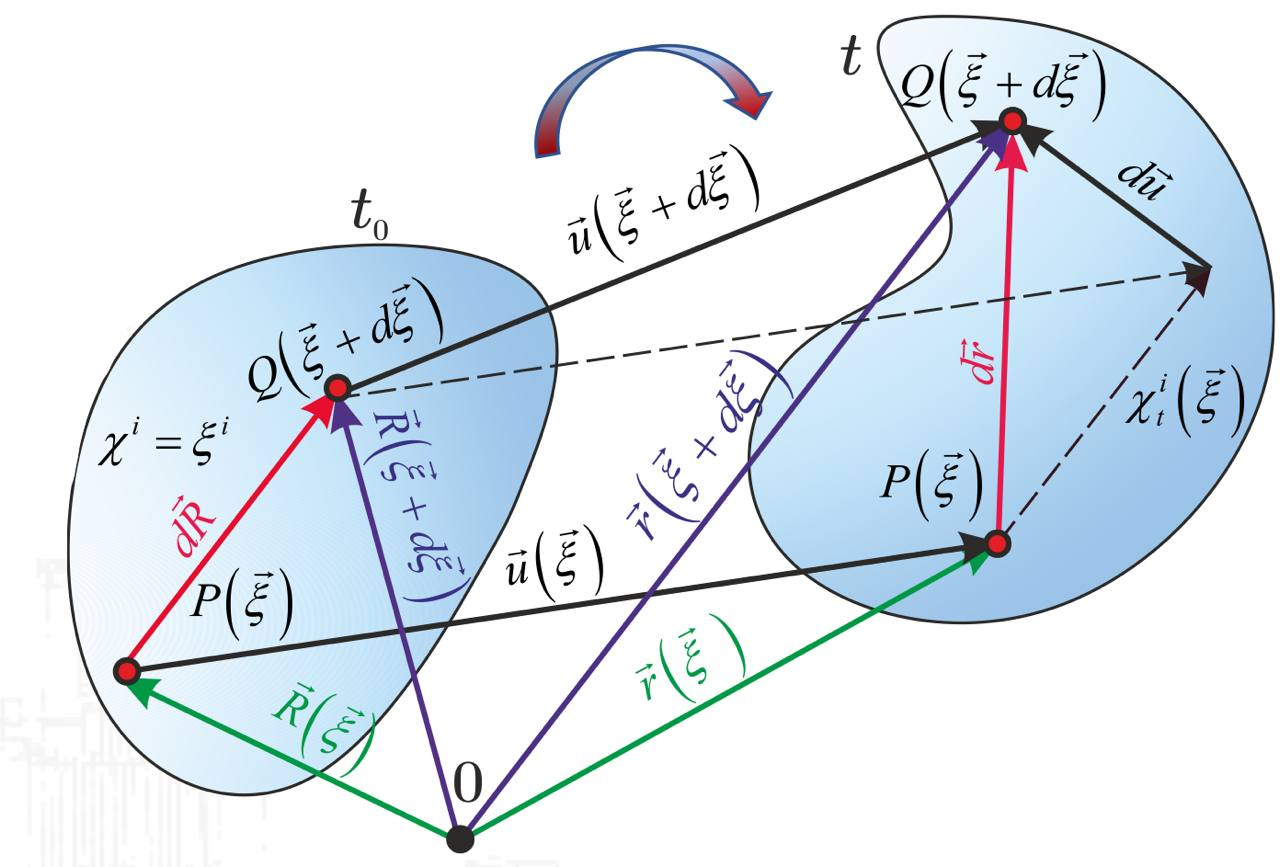
\includegraphics[width=0.6\textwidth]{images/10.1.jpg}
\end{figure}


Рассмотрим два состояния и не будем записывать зависимость от времени. Начальный радиус-вектор выражен через криволинейные координаты:
$$
\vec{R}=\vec{R}(\vec{\xi}) \Leftrightarrow X_i=X_i\left(\xi^1, \xi^2, \xi^3\right)
$$
При Лагранжевском подходе исходим из закона движения:

$$
\vec{r}=\vec{r}(\vec{\xi}) \Leftrightarrow x_i=x_i\left(\xi^1, \xi^2, \xi^3\right)
$$
Элементарный вектор до и после деформации:
$$
\begin{gathered}
d \vec{R}=\frac{\partial \vec{R}}{\partial \xi^i} d \xi^i=\vec{E}_i d \xi^i, d \vec{r}=\frac{\partial \vec{r}}{\partial \xi^i} d \xi^i=\vec{e}_i d \xi^i \\
|d \vec{R}|^2=d \vec{R} \cdot d \vec{R}=\left(\vec{E}_i d \xi^i\right) \cdot\left(\vec{E}_j d \xi^j\right)=\left(\vec{E}_i \cdot \vec{E}_j\right) d \xi^i d \xi^j=G_{i j} d \xi^i d \xi^j \\
|d \vec{r}|^2=d \vec{r} \cdot d \vec{r}=\left(\vec{e}_i d \xi^i\right) \cdot\left(\vec{e}_j d \xi^j\right)=\left(\vec{e}_i \cdot \vec{e}_j\right) d \xi^i d \xi^j=g_{i j} d \xi^i d \xi^j \\
|d \vec{r}|^2-|d \vec{R}|^2=g_{i j} d \xi^i d \xi^j-G_{i j} d \xi^i d \xi^j=2 \Gamma_{i j} d \xi^i d \xi^j \\
\Gamma_{i j}=\frac{g_{i j}-G_{i j}}{2}
\end{gathered}
$$

$
\displaystyle
\text { Материальный градиент: } \vec{\nabla}_{\bar{R}} \equiv \vec{E}^\alpha \partial / \partial \xi^\alpha$Выразим тензор Грина через вектор перемещения:


$
\displaystyle
\vec{r}=\vec{R}+\vec{u} \Rightarrow \vec{\nabla}_{\vec{R}} \overrightarrow{\mathbf{r}}=\vec{\nabla}_{\vec{R}} \overrightarrow{\mathbf{R}}+\vec{\nabla}_{\vec{R}} \overrightarrow{\mathbf{u}} \Leftrightarrow \vec{E}^\alpha \frac{\partial \overrightarrow{\mathbf{r}}}{\partial \xi^\alpha}=\underset{\sim}{\mathbf{E}}+\vec{\nabla}_{\vec{R}} \overrightarrow{\mathbf{u}} \Leftrightarrow \overrightarrow{\mathbf{E}}^\alpha \overrightarrow{\mathbf{e}}_\alpha=\underset{\sim}{\mathbf{E}}+\vec{\nabla}_{\vec{R}} \overrightarrow{\mathbf{u}}, \quad\left(\overrightarrow{\mathbf{E}}^\beta \overrightarrow{\mathbf{e}}_\beta\right)^{\mathbf{T}}=\overrightarrow{\mathbf{e}}_\beta \overrightarrow{\mathbf{E}}^\beta=\underset{\sim}{\mathbf{E}}+\overrightarrow{\mathbf{u}} \vec{\nabla}_{\bar{R}}
$

$\underset{\sim}{\mathbf{g}_{\bar{R}}}=g_{\alpha \beta} \overrightarrow{\mathbf{E}}^\alpha \overrightarrow{\mathbf{E}}^\beta=\underline{\overrightarrow{\mathbf{E}}^\alpha \overrightarrow{\mathbf{e}}_\alpha \cdot \overrightarrow{\mathbf{e}}_\beta \overrightarrow{\mathbf{E}}^\beta}=\left(\underset{\sim}{\mathbf{E}}+\vec{\nabla}_{\vec{R}} \overrightarrow{\mathbf{u}}\right) \cdot\left(\underset{\sim}{\mathbf{E}}+\overrightarrow{\mathbf{u}} \vec{\nabla}_{\bar{R}}\right)=\underset{\sim}{\mathbf{E}}+\vec{\nabla}_{\bar{R}} \overrightarrow{\mathbf{u}}+\overrightarrow{\mathbf{u}} \vec{\nabla}_{\vec{R}}+\vec{\nabla}_{\vec{R}} \overrightarrow{\mathbf{u}} \cdot \overrightarrow{\mathbf{u}} \vec{\nabla}_{\vec{R}}$

$\displaystyle \underset{\sim}{\Gamma}=\frac{1}{2}\left(\mathbf{g}_{\vec{R}}-\underset{\sim}{\mathbf{E}}\right) \Rightarrow \underset{\sim}{\Gamma}=\frac{1}{2}\left(\vec{\nabla}_{\vec{R}} \overrightarrow{\mathbf{u}}+\overrightarrow{\mathbf{u}} \vec{\nabla}_{\vec{R}}+\vec{\nabla}_{\vec{R}} \overrightarrow{\mathbf{u}} \cdot \overrightarrow{\mathbf{u}} \vec{\nabla}_{\vec{R}}\right) \Leftrightarrow \Gamma_{i j}=\frac{1}{2}\left(u_{j, i}+u_{i, j}+u_{q, i} u_{, j}^q\right)$

Обозначим единичные направляющие вектора до и после деформирования как $\vec{\tau}, \hat\vec{\tau}$

\begin{figure}[h!]
  \centering
  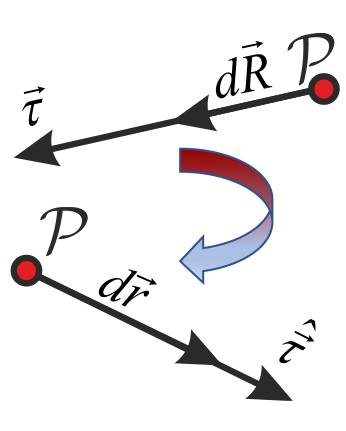
\includegraphics[width=0.2\textwidth]{images/10.2.jpg}
\end{figure}


$$
\begin{aligned}
& \vec{\tau}=\left(\tau^1, \tau^2, \tau^3\right)_{\vec{R}}=\frac{d \vec{R}}{|d \vec{R}|}=\frac{d \xi^1}{|d \vec{R}|} \vec{E}_1+\frac{d \xi^2}{|d \vec{R}|} \vec{E}_2+\frac{d \xi^3}{|d \vec{R}|} \vec{E}_3 \Rightarrow \tau^i=\frac{d \xi^i}{|d \vec{R}|},|\vec{\tau}|=\sqrt{\tau^i \tau^j G_{i j}}=1 \\
& \hat{\vec{\tau}}=\left(\hat{\tau}_{\vec{r}}^1, \hat{\tau}_{\vec{r}}^2, \hat{\tau}_{\vec{r}}^3\right)_{\vec{r}}=\frac{d \vec{r}}{|d \vec{r}|}=\frac{d \xi^1}{|d \vec{r}|} \vec{e}_1+\frac{d \xi^2}{|d \vec{r}|} \vec{e}_2+\frac{d \xi^3}{|d \vec{r}|} \vec{e}_3 \Rightarrow \hat{\tau}_{\vec{r}}^i=\frac{d \xi^i}{|d \vec{r}|},|\hat{\vec{\tau}}|=\sqrt{\hat{\tau}_{\vec{r}}^i \hat{\tau}_{\vec{r}}^j g_{i j}}=1 \\
&|d \vec{r}|^2-|d \vec{R}|^2=2 \Gamma_{i j} d \xi^i d \xi^j \Leftrightarrow \frac{|d \vec{r}|}{|d \vec{R}|}=\sqrt{1+2 \Gamma_{i j} \frac{d \xi^i}{|d \vec{R}|} \frac{d \xi^j}{|d \vec{R}|}}=\sqrt{1+2 \Gamma_{i j} \tau^i \tau^j} \Leftrightarrow\\
&|d \vec{r}|=\sqrt{1+2 \cdot \Gamma_{i j} \tau^i \tau^j|d \vec{R}|}
\end{aligned}
$$
 Относительное изменение длины элементарного волокна в заданном направлении $\vec{\tau}$:

$$
\lambda(\vec{\tau})=\frac{|d \vec{r}|-|d \vec{R}|}{|d \vec{R}|}=\frac{|d \vec{r}|}{|d \vec{R}|}-1=\sqrt{1+2 \cdot \Gamma_{i j} \tau^i \tau^j}-1 \Rightarrow \begin{aligned}
& \lambda(\vec{\tau})=\sqrt{1+2 \cdot \Gamma_{i j} \tau^i \tau^j}-1 
\end{aligned}
$$
\textbf{Изменения угла между двумя элементарными волокнами} 


Выразим компоненты единичных векторов через лагранжевы компоненты $ u^i$  вектора перемещения т.P  

\begin{figure}[h!]
  \centering
  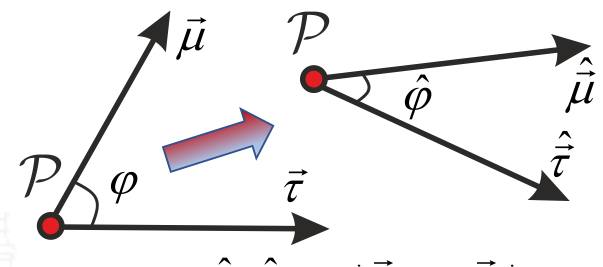
\includegraphics[width=0.4\textwidth]{images/10.3.jpg} 
\end{figure}



$ d \vec{r}=d \vec{R}+d \vec{u}=\frac{\partial \vec{R}}{\partial \xi^m} d \xi^m+\frac{\partial \vec{u}}{\partial \xi^i} d \xi^i=\vec{E}_m d \xi^m+u_{, i}^m \vec{E}_m d \xi^i=\left(\delta_i^m d \xi^i+u_{, i}^m d \xi^i\right) \vec{E}_m=\left(\delta_i^m+u_{, i}^m\right) d \xi^i \vec{E}_m$


$
\begin{gathered}
\frac{d \xi^i}{|d \vec{R}|}=\tau^i, \quad|d \vec{r}|=\sqrt{1+2 \cdot \Gamma_{i j} \tau^i \tau^j}|d \vec{R}|, \quad d \vec{r}=\left(\delta_i^m+u_i^m\right) d \xi^i \cdot \vec{E}_m \\
\vec{\tau}=\tau^i \overrightarrow{E_i}, \quad \hat{\vec{\tau}}=\frac{d \vec{r}}{|d \vec{r}|}=\frac{\left(\delta_i^m+u_i^m\right) d \xi^i \cdot \vec{E}_m}{\sqrt{1+2 \Gamma_{i j} \tau^i \tau^j}|d \vec{R}|}=\frac{\left(\delta_i^m+u_i^m\right) \tau^i}{1+\lambda(\vec{\tau})} \vec{E}_m \equiv \hat{\tau}^m \vec{E}_m
\end{gathered}
$
$
\begin{aligned}
& \vec{\mu}=\mu^j \vec{E}_j, \quad \hat{\vec{\mu}}=\frac{\left(\delta_j^m+u_{, j}^m\right) \mu^j}{1+\lambda(\vec{\mu})} \vec{E}_m=\frac{\left(\delta_j^m+u_{, j}^m\right) \mu^j}{1+\lambda(\vec{\mu})} G_{m k} \vec{E}^k=\frac{\left(\delta_j^m G_{m k}+u_{, j}^m G_{m k}\right) \mu^j}{1+\lambda(\vec{\mu})} \vec{E}^k=\\
& =\frac{\left(G_{j k}+u_{k, j}\right) \mu^j}{1+\lambda(\vec{\mu})} \vec{E}^k \equiv \hat{\mu}_k \vec{E}^k \\
& \cos \hat{\varphi}=\hat{\tau}^k \hat{\mu}_k=\frac{\left(\delta_i^k+u_{, i}^k\right) \tau^i}{1+\lambda(\vec{\tau})} \frac{\left(G_{j k}+u_{k, j}\right) \mu^j}{1+\lambda(\vec{\mu})}=\frac{\left(G_{j k} \delta_i^k+\delta_i^k u_{k, j}+u_{, i}^k G_{j k}+u_{i, i}^k u_{k, j}\right) \tau^i \mu^j}{(1+\lambda(\vec{\tau}))(1+\lambda(\vec{\mu}))}=\\
& =\frac{\left(G_{j i}+u_{i, j}+u_{j, i}+u_{i, i}^k u_{k, j}\right) \tau^i \mu^j}{(1+\lambda(\vec{\tau}))(1+\lambda(\vec{\mu}))}
\end{aligned}
$
$\begin{aligned} \cos \hat{\varphi} & =\frac{\left(G_{j i}+u_{i, j}+u_{j, i}+u_{j i}^k u_{k, j}\right) \tau^i \mu^j}{(1+\lambda(\vec{\tau}))(1+\lambda(\vec{\mu}))}=\frac{\left(G_{i j}+2 \cdot \Gamma_{i j}\right) \tau^i \mu^j}{(1+\lambda(\vec{\tau}))(1+\lambda(\vec{\mu}))} =\frac{G_{i j} \tau^i \mu^j+2 \cdot \Gamma_{i j} \tau^i \mu^j}{(1+\lambda(\vec{\tau}))(1+\lambda(\vec{\mu}))} \\ \cos \hat{\varphi} & =\frac{\cos \varphi+2 \cdot \Gamma_{i j} \tau^i \mu^j}{(1+\lambda(\vec{\tau}))(1+\lambda(\vec{\mu}))}.\end{aligned}$


\textbf{Относительного изменения элементарного объема (дилатация)}


В точке $\left(\xi^1, \xi^2, \xi^3\right) \in V_0$ рассмотрим тройку элементарных векторов $d \vec{R}_{(\alpha)}=d \xi_{(\alpha)}^i \vec{E}_i, \alpha=1,2,3$ Объем косого параллелепипеда, построенного на этих векторах равен: 

\begin{figure}[h!]
  \centering
  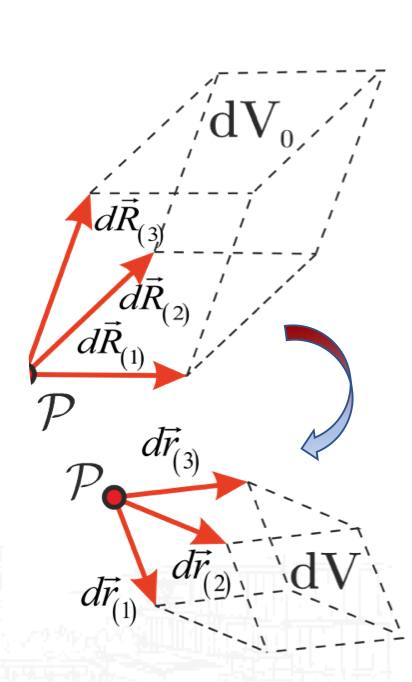
\includegraphics[width=0.3\textwidth]{images/10.4.jpg} 
\end{figure}

$$
\begin{aligned}
& d V_0=d \vec{R}_{(1)} \cdot\left(d \vec{R}_{(2)} \times d \vec{R}_{(3)}\right)=\left(d \xi_{(1)}^i \vec{E}_i\right) \cdot\left(\left(d \xi_{(2)}^j \vec{E}_j\right) \times\left(d \xi_{(3)}^k \vec{E}_k\right)\right)= \\
& =\vec{E}_i \cdot\left(\vec{E}_j \times \vec{E}_k\right) d \xi_{(1)}^i d \xi_{(2)}^j d \xi_{(3)}^k=\Xi_{i j k} d \xi_{(1)}^i d \xi_{(2)}^j d \xi_{(3)}^k=\sqrt{G} \cdot e_{i j k} d \xi_{(1)}^i d \xi_{(2)}^j d \xi_{(3)}^k
\end{aligned}
$$
После деформации косой параллелепипед становится построенным на векторах $d \vec{r}_{(\alpha)}=d \xi_{(\alpha)}^i \vec{e}_i$, в которые переходят векторы $d \vec{R}_{(\alpha)}$. Частицы, расположенные до деформации в объеме $d V_0$, после деформации займут объем $d V$, равный:
$$
\begin{aligned}
& d V=d \vec{r}_{(1)} \cdot\left(d \vec{r}_{(2)} \times d \vec{r}_{(3)}\right)=\left(d \xi_{(1)}^i \vec{e}_i\right) \cdot\left(\left(d \xi_{(2)}^j \vec{e}_j\right) \times\left(d \xi_{(3)}^k \vec{e}_k\right)\right)= \\
& =\vec{e}_i \cdot\left(\vec{e}_j \times \vec{e}_k\right) d \xi_{(1)}^i d \xi_{(2)}^j d \xi_{(3)}^k=\varepsilon_{i j k} d \xi_{(1)}^i d \xi_{(2)}^j d \xi_{(3)}^k=\sqrt{g} \cdot e_{i j k} d \xi_{(1)}^i d \xi_{(2)}^j d \xi_{(3)}^k\\
&
 \theta \equiv \frac{d V-d V_0}{d V_0}=\frac{d V}{d V_0}-1=\sqrt{\frac{g}{G}}-1
\end{aligned}
$$
$\displaystyle
\sqrt{g}=\vec{e}_1 \cdot\left(\vec{e}_2 \times \vec{e}_3\right)=\left[\left(\delta_1^i+u_{, 1}^i\right) \vec{E}_i\right] \cdot\left[\left(\left(\delta_2^j+u_{, 2}^j\right) \vec{E}_j\right) \times\left(\left(\delta_3^k+u_{, 3}^k\right) \vec{E}_k\right)\right]=\left(\delta_1^i+u_{, 1}^i\right)\left(\delta_2^j+u_{, 2}^j\right)\left(\delta_3^k+u_{, 3}^k\right) \vec{E}_i \cdot\left(\vec{E}_j \times \vec{E}_k\right) =\left(\delta_1^i+u_{, 1}^i\right)\left(\delta_2^j+u_{, 2}^j\right)\left(\delta_3^k+u_{, 3}^k\right) \Xi_{i j k}=\left(\delta_1^i+u_{, 1}^i\right)\left(\delta_2^j+u_{, 2}^j\right)\left(\delta_3^k+u_{, 3}^k\right) e_{i j k} \sqrt{G}=\mathrm{det}\left(\delta_p^q+u_{, p}^q\right) \sqrt{G}=\mathrm{det}\left[\underset{\sim}{\mathbf{E}}+\vec{\nabla}_{\vec{R}} \overrightarrow{\mathbf{u}}\right] \sqrt{G}=\mathrm{det} \underset{\sim}{\mathbf{B}} \cdot \sqrt{G}, \quad \underset{\sim}{\mathbf{B}} \equiv \underset{\sim}{\mathbf{E}}+\vec{\nabla}_{\vec{R}} \overrightarrow{\mathbf{u}}
$
$$
\left[B_i^{\cdot j}\right]=\left(\begin{array}{ccc}
1+u_{, 1}^1 & u_{, 1}^2 & u_{, 1}^3 \\
u_{, 2}^1 & 1+u_{, 2}^2 & u_{, 2}^3 \\
u_{, 3}^1 & u_{, 3}^2 & 1+u_{, 3}^3
\end{array}\right)
$$
$
\displaystyle
\mathrm{det}^2 \underset{\sim}{\mathbf{B}}=\mathrm{det} \underset{\sim}{\mathbf{B}} \cdot \mathrm{det} \underset{\sim}{\mathbf{B}}=\mathrm{det} \underset{\sim}{\mathbf{B}} \cdot \mathrm{det} \underset{\sim}{\mathbf{B}}=\mathrm{det}(\underset{\sim}{\mathbf{B}} \cdot \underset{\sim}{\mathbf{B}})=\mathrm{det}\left(\underset{\sim}{\mathbf{E}}+\vec{\nabla}_{\vec{R}} \overrightarrow{\mathbf{u}}\right) \cdot\left(\underset{\sim}{\mathbf{E}}+\vec{\nabla}_{\vec{R}} \overrightarrow{\mathbf{u}}\right)^{\mathrm{T}}=\mathrm{det}\left(\underset{\sim}{\mathbf{E}}+\vec{\nabla}_{\vec{R}} \overrightarrow{\mathbf{u}}\right) \cdot\left(\underset{\sim}{\mathbf{E}}+\overrightarrow{\mathbf{u}} \vec{\nabla}_{\vec{R}}\right)=\mathrm{det}\left(\underset{\sim}{\mathbf{E}}+\vec{\nabla}_{\vec{R}} \overrightarrow{\mathbf{u}}+\overrightarrow{\mathbf{u}} \vec{\nabla}_{\bar{R}}+\vec{\nabla}_{\bar{R}} \overrightarrow{\mathbf{u}} \cdot \overrightarrow{\mathbf{u}}_{\bar{R}}\right)=\mathrm{det}\left(\underset{\sim}{\mathbf{E}}+\vec{\nabla}_{\vec{R}} \overrightarrow{\mathbf{u}}+\overrightarrow{\mathbf{u}} \vec{\nabla}_{\vec{R}}+\vec{\nabla}_{\vec{R}} \overrightarrow{\mathbf{u}} \cdot \overrightarrow{\mathbf{u}}_{\bar{R}}\right)=\mathrm{det}\left(\underset{\sim}{\mathbf{E}}+2 \cdot \Gamma_{\sim}\right) g / G=\mathrm{det}^2 \underset{\sim}{\mathbf{B}}=\mathrm{det}(\underset{\sim}{\mathbf{E}}+2 \cdot \underset{\sim}{\Gamma})=\mathrm{det}\left[\delta_j^i+2 \Gamma_j^i\right]=e_{i j k}\left(\delta_1^i+2 \Gamma_1^i\right)\left(\delta_2^j+2 \Gamma_2^j\right)\left(\delta_3^k+2 \Gamma_3^k\right)=e_{i j k} \delta_1^i \delta_2^j \delta_3^k +8 e_{i j k} \Gamma_1^i \Gamma_2^j \Gamma_3^k+2 e_{i j k}\left(\delta_1^i \delta_2^j \Gamma_3^k+\delta_1^i \delta_3^k \Gamma_2^j+\delta_2^j \delta_3^k \Gamma_1^i\right)+4 e_{i j k}\left(\delta_1^i \Gamma_2^j \Gamma_3^k+\delta_2^j \Gamma_1^i \Gamma_3^k+\delta_3^k \Gamma_1^i \Gamma_2^j\right)=e_{123}+8 \mathrm{det}\left\|\Gamma_j^i\right\| +2\left(e_{12 k} \Gamma_3^k+e_{1 j 3} \Gamma_2^j+e_{i 23} \Gamma_1^i\right)+4\left(e_{1 j k} \Gamma_2^j \Gamma_3^k+e_{i 2 k} \Gamma_1^i \Gamma_3^k+e_{i j 3} \Gamma_1^i \Gamma_2^j\right)=1+8 \Pi_{\Gamma}+2\left(\Gamma_3^3+\Gamma_2^2+\Gamma_1^1\right) +2\left(2\left(\Gamma_2^2 \Gamma_3^3-\Gamma_2^3 \Gamma_3^2\right)+2\left(\Gamma_1^1 \Gamma_3^3-\Gamma_1^3 \Gamma_3^1\right)+2\left(\Gamma_1^1 \Gamma_2^2-\Gamma_2^2 \Gamma_1^1\right)\right)=1+2 \mathrm{I}_{\Gamma}+4 \Pi_{\Gamma}+8 \Pi_{\Gamma} \text {. } $
$$
\theta \equiv \frac{d V-d V_0}{d V_0}=\sqrt{\frac{g}{G}}-1=\sqrt{1+2 \mathrm{I}_{\Gamma}+4 \mathrm{I}_{\Gamma}+8 \mathrm{III}_{\Gamma}}-1
$$


Для описания малых деформаций
применяется тензор малых деформаций Коши: Деформации и вращения считаются малыми если все компоненты тензора дисторсии существенно меньше единицы по абсолютной величине $\left|d_{i j}\right|=\left|u_{j, i}\right| \ll 1$. В этом случае в $\Gamma_{i j}=\frac{1}{2}\left(u_{j, i}+u_{i, j}+u_{q, i} u_{, j}^q\right)$ можно пренебречь квадратичными слагаемыми по сравнению с линейными составляющими и тогда $\Gamma_{i j} \approx \varepsilon_{i j}=\frac{1}{2}\left(u_{j, i}+u_{i, j}\right)$. 


Получаем: \textbf{тензор малых деформаций Коши} $\varepsilon_{i j}=1 / 2\left(u_{j, i}+u_{i, j}\right)$ 
\textbf{, тензор малых поворотов}: $\omega_{i j}=1 / 2\left(u_{j, i}-u_{i, j}\right)$


\section{Формулы Чезаро. Уравнения совместности Сен-Венана.}
\textbf{Формулы Чезаро:}


Во всех точках тела известно поле деформаций $\varepsilon_{i j}\left(x_i\right)$. В точке $O\left(x_i^o\right)$ известны перемещения $u_i^O$ и вращения $\omega_{i j}^O$. Требуется найти перемещения в точке $P\left(x_i^P\right)$. 

\begin{figure}[h!]
  \centering
  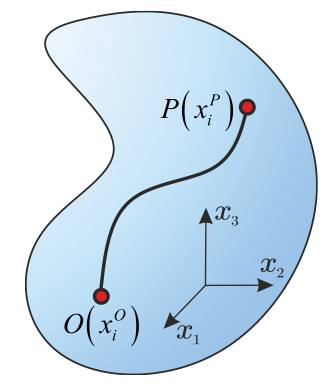
\includegraphics[width=0.3\textwidth]{images/11.1.jpg} 
\end{figure}


Перемещения в точке бесконечно близкой к точке О можно найти по формуле $u_i=u_i^O+d u_i=u_i^O+u_{i, j} d x_j=u_i^O+\left(\varepsilon_{i j}+\omega_{j i}\right) d x_j$. Соединим точки $O$ и $P$ кривой, лежащей целиком в теле. Тогда перемещения в произвольной точке $P$ будут равны
$$
u_i^p=u_i^O+\int_{O P} d u_i=u_i^O+\int_{x_j^O}^{x_j^P} u_{i, j} d x_j=u_i^O+\int_O^P\left(\varepsilon_{i j}+\omega_{j i}\right) d x_j=u_i^O+\int_O^P \varepsilon_{i j} d x_j+\int_O^P \omega_{j i} d x_j
$$
Сначала докажем тождество: $\omega_{j i, k} \equiv \varepsilon_{i k, j}-\varepsilon_{k j, i}$. 


Используем: $\varepsilon_{i j} \equiv \frac{1}{2}\left(u_{i, j}+u_{j, i}\right), \omega_{j i} \equiv \frac{1}{2}\left(u_{i, j}-u_{j, i}\right)$.
$$
\begin{aligned}
\omega_{j i, k} & =\frac{1}{2}\left(u_{i, j k}-u_{j, i k}\right)=\frac{1}{2}\left(u_{i, j k}+u_{k, j i}-u_{k, j i}-u_{j, i k}\right)=\frac{1}{2}\left(u_{i, k j}+u_{k, i j}\right)- \\
& -\frac{1}{2}\left(u_{k, j i}+u_{j, k i}\right)=\frac{1}{2}\left(u_{i, k}+u_{k, i}\right)_{, j}-\frac{1}{2}\left(u_{k, j}+u_{j, k}\right)_{, i}=\varepsilon_{i k, j}-\varepsilon_{k j, i}
\end{aligned}
$$
Проинтегрируем по частям, используя  $\omega_{j i}^P-\omega_{j i}^o=\int_0^P \omega_{j i, k} d x_k$
$
\displaystyle
\int_O^P \omega_{j i} d x_j=\left.\omega_{j i} x_j\right|_O ^P-\int_O^P x_j \omega_{j i, k} d x_k=\omega_{j i}^P x_j^P-\omega_{j i}^O x_j^O-\int_O^P x_j \omega_{j i, k} d x_k=\omega_{j i}^O\left(x_j^P-x_j^O\right)+\left(\omega_{j i}^P-\omega_{j i}^O\right) x_j^P
-\int_O^P x_j \omega_{j i, k} d x_k=\omega_{j i}^O\left(x_j^P-x_j^O\right)+x_j^P \int_O^P \omega_{j i, k} d x_k-\int_O^P x_j \omega_{j i, k} d x_k=\omega_{j i}^O\left(x_j^P-x_j^O\right)+\int_O^P\left(x_j^P-x_j\right) \omega_{j i, k} d x_k 
=\omega_{j i}^O\left(x_j^P-x_j^O\right)+\int_O^P\left(x_j^P-x_j\right)\left(\varepsilon_{i k, j}-\varepsilon_{k j, i}\right) d x_k \stackrel{j \leftrightarrow k}{=} \omega_{j i}^O\left(x_j^P-x_j^O\right)+\int_O^P\left(x_k^P-x_k\right)\left(\varepsilon_{i j, k}-\varepsilon_{j k, i}\right) d x_j.$


$ \displaystyle
u_i^P=u_i^O+\omega_{j i}^O\left(x_j^P-x_j^O\right)+\int_O^P\left[\varepsilon_{i j}+\left(x_k^P-x_k\right)\left(\varepsilon_{i j, k}-\varepsilon_{j k, i}\right)\right] d x_j.
$


\textbf{Соотношения (уравнения) совместности Сен-Венана:}


 Обозначим $\Psi_{i j}=\varepsilon_{i j}+\left(x_k^P-x_k\right)\left(\varepsilon_{i j, k}-\varepsilon_{j k, i}\right)$. Для того, чтобы $\vec{u}$ было векторным полем значение интеграла в формулах Чезаро не должно зависеть от выбора пути интегрирования, а зависит только от выбора точек $O$ и P, т.е: $\oint \Psi_{i j} d x_j=0 \Leftrightarrow \Psi_{i j, l}=\Psi_{i l,j}$
$$
\begin{aligned}
& \left(\varepsilon_{i j}+\left(x_k^P-x_k\right)\left(\varepsilon_{i j, k}-\varepsilon_{j k, i}\right)\right)_{, l}=\left(\varepsilon_{i l}+\left(x_k^P-x_k\right)\left(\varepsilon_{i l, k}-\varepsilon_{l k, i}\right)\right)_{, j} \\
& \varepsilon_{i j, l}-x_{k, l}\left(\varepsilon_{i j, k}-\varepsilon_{j k, i}\right)+\left(x_k^P-x_k\right)\left(\varepsilon_{i j, k l}-\varepsilon_{j k, i l}\right)=\varepsilon_{i l, j}-x_{k, j}\left(\varepsilon_{i l, k}-\varepsilon_{l k, i}\right)+ \\&+\left(x_k^P-x_k\right)\left(\varepsilon_{i l, k j}-\varepsilon_{l k, i j}\right) \\
& \left(x_k^P-x_k\right)\left(\varepsilon_{i j, k l}-\varepsilon_{j k, i l}-\varepsilon_{i l, k j}+\varepsilon_{l k, i j}\right)=\varepsilon_{i l, j}-\delta_{k j}\left(\varepsilon_{i l, k}-\varepsilon_{l k, i}\right)-\varepsilon_{i j, l}+\delta_{k l}\left(\varepsilon_{i j, k}-\varepsilon_{j k, i}\right) \\
& \left(x_k^P-x_k\right)\left(\varepsilon_{i j, k l}-\varepsilon_{j k, i l}-\varepsilon_{i l, k j}+\varepsilon_{l k, i j}\right)=\varepsilon_{i l, j}-\varepsilon_{i l, j}+\varepsilon_{l j, i}-\varepsilon_{i j, l}+\varepsilon_{i j, l}-\varepsilon_{j l, i}=0 \\
& \text { Получаем } 81 \text { формулу: } \quad \varepsilon_{i j, k l}-\varepsilon_{j k, i l}-\varepsilon_{i l, k j}+\varepsilon_{l k, i j}=0, i, j, k, l=1,2,3.
\end{aligned}
$$


Обозначим $\chi_{i j k l} \equiv \varepsilon_{i j, k l}-\varepsilon_{j k, i l}-\varepsilon_{i l, k j}+\varepsilon_{l k, i j}$ и определим его независимые компоненты. 

Переставляем индексы исходя из симметрии:


а) индексы $1 \leftrightarrow 3: \quad \chi_{k j i l}=\varepsilon_{k j, i l}-\varepsilon_{j i, k l}-\varepsilon_{k l, i j}+\varepsilon_{l i, k j}=-\chi_{i j k l}$. (Независимых 27)


б) индексы $2 \leftrightarrow 4: \quad \chi_{i l k j}=\varepsilon_{i l, k j}-\varepsilon_{l k, i j}-\varepsilon_{i j, k l}+\varepsilon_{j k, i l}=-\chi_{i j k l}$. (Независимых 9)
в) индексы $1 \leftrightarrow 2$ и $3 \leftrightarrow 4: \chi_{j i l k}=\varepsilon_{j i, l k}-\varepsilon_{i l, j k}-\varepsilon_{j k, l i}+\varepsilon_{k l, j i}=\chi_{i j k l}$. (Независимых 6)
Независимые компоненты: $\chi_{\underline{1} \underline{12} 2}, \chi_{\underline{1} 123}, \chi_{\underline{1} 1 \underline{3} 3}, \chi_{\underline{1} 2 \underline{2} 3}, \chi_{\underline{2} 2 \underline{3} 3}, \chi_{\underline{1} 2 \underline{3} 3}$.
$$
\begin{aligned}
& \chi_{1122}=\varepsilon_{11,22}-\varepsilon_{12,12}-\varepsilon_{12,21}+\varepsilon_{22,11}=0 ; \quad \chi_{1123}=\varepsilon_{11,23}-\varepsilon_{12,13}-\varepsilon_{13,21}+\varepsilon_{32,11}=0 \\
& \chi_{1133}=\varepsilon_{11,33}-\varepsilon_{13,13}-\varepsilon_{13,31}+\varepsilon_{33,11}=0 ; \quad \chi_{1223}=\varepsilon_{12,23}-\varepsilon_{22,13}-\varepsilon_{13,22}+\varepsilon_{32,12}=0 \\
& \chi_{2233}=\varepsilon_{22,33}-\varepsilon_{23,23}-\varepsilon_{23,32}+\varepsilon_{33,22}=0 ; \quad \chi_{1233}=\varepsilon_{12,33}-\varepsilon_{23,13}-\varepsilon_{13,23}+\varepsilon_{33,12}=0 \\
& \left\{\begin{array}{l}
\varepsilon_{11,22}+\varepsilon_{22,11}=2 \varepsilon_{12,12} \\
\varepsilon_{11,33}+\varepsilon_{33,11}=2 \varepsilon_{13,13} \\
\varepsilon_{22,33}+\varepsilon_{33,22}=2 \varepsilon_{23,23}
\end{array} ;\left\{\begin{array}{l}
\left(\varepsilon_{12,3}-\varepsilon_{23,1}+\varepsilon_{31,2}\right)_{, 1}=\varepsilon_{11,23} \\
\left(\varepsilon_{12,3}+\varepsilon_{23,1}-\varepsilon_{31,2}\right)_{, 2}=\varepsilon_{22,13} \\
\left(-\varepsilon_{12,3}+\varepsilon_{23,1}+\varepsilon_{31,2}\right)_{, 3}=\varepsilon_{33,12}
\end{array}\right.\right. 
\end{aligned}
$$
Соотношения
(уравнения)
Сен-Венана:
$$
\left\{\begin{array}{l}
\varepsilon_{11,22}+\varepsilon_{22,11}=2 \varepsilon_{12,12} \\
\varepsilon_{11,33}+\varepsilon_{33,11}=2 \varepsilon_{13,13} \\
\varepsilon_{22,33}+\varepsilon_{33,22}=2 \varepsilon_{23,23}
\end{array} ;\left\{\begin{array}{l}
\left(\varepsilon_{12,3}-\varepsilon_{23,1}+\varepsilon_{31,2}\right)_{, 1}=\varepsilon_{11,23} \\
\left(\varepsilon_{12,3}+\varepsilon_{23,1}-\varepsilon_{31,2}\right)_{, 2}=\varepsilon_{22,13} \\
\left(-\varepsilon_{12,3}+\varepsilon_{23,1}+\varepsilon_{31,2}\right)_{, 3}=\varepsilon_{33,12}
\end{array}\right.\right.
$$


\section{Обобщенный изотермический линейный закон Гука. Потенциал линейно-упругого тела.  Три общих типа симметрии упругих констант. Три специальных типа симметрии: ортотропный, трансверсально-изотропный и изотропный материалы. Материальные константы Ламе. Технические константы. Формулы, которые связывают константы Ламе и технические константы.}

\begin{figure}[h!]
  \centering
  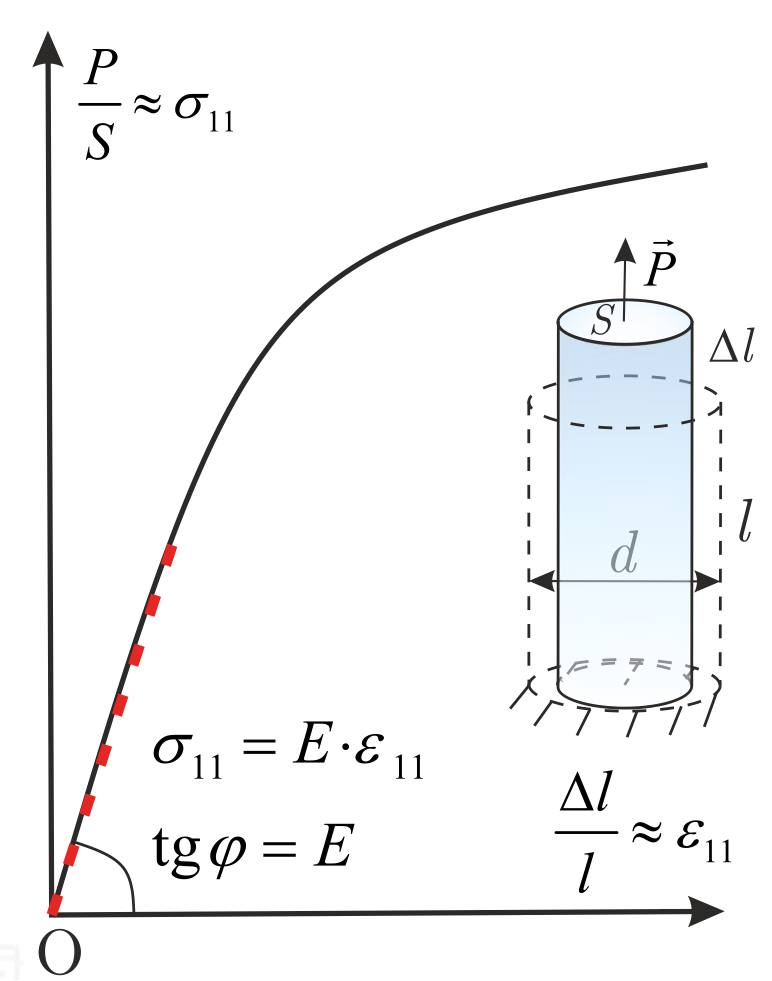
\includegraphics[width=0.4\textwidth]{images/12.1.jpg} 
\end{figure}


В упругом теле приложение нагрузки приводит к мгновенному появлению деформаций в теле, которые не изменяются с течением времени и полностью исчезают после снятия нагрузки. Связь между напряжениями и деформациями может быть нелинейной. Однако многие материалы при небольших нагрузках показывают линейную зависимость напряжений от деформаций. Такие материалы называются \textbf{линейно-упругими материалами.}  При постоянной температуре линейные связи $\underset{\sim}{\sigma} \sim \underset{\sim}{\mathcal{E}}$ и $\underset{\sim}{\mathcal{E}} \sim \underset{\sim}{\sigma}$ осуществляются с помощью тензоров четвертого ранга: ( $\tenq{\mathbf{C}}$ - тензор упругих модулей; $ \tenq{\mathbf{J}}$ - тензор упругих податливостей). 
$$
\begin{aligned}
& \underset{\sim}{\sigma}=\tenq{\mathbf{C}}: \underset{\sim}{\mathcal{E}} \equiv {\tenq{\mathbf{C}}} \cdot \cdot \underset{\sim}{\mathcal{E}} \Leftrightarrow \underset{\sim}{\mathcal{E}}=\tenq{\mathbf{J}}: \underset{\sim}{\sigma} \equiv \tenq{\mathbf{J}} \cdot\cdot\underset{\sim}{\sigma}\\
& \sigma^{i j}(\vec{x})=C^{i j k l}(\vec{x}) \varepsilon_{k l}(\vec{x}) \Leftrightarrow \varepsilon_{k l}(\vec{x})=J_{k l i j}(\vec{x}) \sigma^{i j}(\vec{x}) \\
& \text{В декартовой системе координат:} \\
& C_{i j p q}=C_{i j q p}, \varepsilon_{p q}=\varepsilon_{q p} \Rightarrow \sigma_{i j}=C_{i j 11} \varepsilon_{11}+C_{i j 22} \varepsilon_{22}+C_{i j 33} \varepsilon_{33}+C_{i j 23}\left(2 \varepsilon_{23}\right)+\\
&+C_{i j 13}\left(2 \varepsilon_{13}\right)+C_{i j 12}\left(2 \varepsilon_{12}\right), i, j=1,2,3 \text{(зав. от 6 компонент } \varepsilon )\\
& (\varepsilon_{11}^*=\varepsilon_{11}, \varepsilon_{22}^*=\varepsilon_{22}, \varepsilon_{33}^*=\varepsilon_{33},  \varepsilon_{12}^*=2 \varepsilon_{12}, \varepsilon_{23}^*=2 \varepsilon_{23}, \varepsilon_{13}^*=2 \varepsilon_{13}) \\
\end{aligned}
$$

Изотермические потенциалы линейно-упругого материала:
$$
W\left(\varepsilon_{k l}^*\right): \sigma^{i j}=\frac{\partial W}{\partial \varepsilon_{i j}^*}, \quad \mathrm{~W}\left(\sigma^{i j}\right): \varepsilon_{i j}^*=\frac{\partial \mathrm{W}}{\partial \sigma^{i j}} \\
$$
 Три общих типа симметрии упругих констант:

 
 1.$\quad
 \begin{aligned} & \frac{\partial^2 W}{\partial \varepsilon_{k l}^* \partial \varepsilon_{i j}^*}=\frac{\partial}{\partial \varepsilon_{k l}^*}\left(\frac{\partial W}{\partial \varepsilon_{i j}^*}\right)=\frac{\partial \sigma^{i j}}{\partial \varepsilon_{k l}^*}=\frac{\partial C^{i j p q} \varepsilon_{p q}}{\partial \varepsilon_{k l}^*}=C^{i j p q} \delta_p^k \delta_q^l=C^{i j k l} \\ & \frac{\partial^2 W}{\partial \varepsilon_{k l}^* \partial \varepsilon_{i j}^*}=\frac{\partial}{\partial \varepsilon_{i j}^*}\left(\frac{\partial W}{\partial \varepsilon_{k l}^*}\right)=\frac{\partial \sigma^{k l}}{\partial \varepsilon_{i j}^*}=\frac{\partial C^{k l p q} \varepsilon_{p q}}{\partial \varepsilon_{i j}^*}=C^{k l p q} \delta_p^i \delta_q^j=C^{k l i j}\end{aligned} \Rightarrow$

 
 $ C^{i j k l}=C^{k l i j} \quad J_{i j k l}=J_{k l i j} \quad W=\frac{1}{2} C^{i j k l} \varepsilon_{i j} \varepsilon_{k l} \quad \mathrm{~W}=\frac{1}{2} J_{i j k l} \sigma^{i j} \sigma^{k l}=W $

2. Симметрирование: $\mathrm{Sym}_{34} \underset{\approx}{\mathbf{C}} \Leftrightarrow C^{i j(k l)}=\frac{1}{2}\left(C^{i j k l}+C^{i j l k}\right)$. 

Альтернирование: $\mathrm{Alt}_{34} \underset{\approx}{\mathbf{C}} \Leftrightarrow C^{i j[k]}=\frac{1}{2}\left(C^{i j k l}-C^{i j l k}\right)$

( свёртка антисимметрично и симметричного)$C^{i j[k l]} \varepsilon_{k l}=0$


 $\Rightarrow C^{i j k l} \varepsilon_{k l}=\left(C^{i j(k l)}+C^{i j[k]]}\right) \varepsilon_{k l}=C^{i j(k l)} \varepsilon_{k l} \Rightarrow C^{i j k l}=C^{i j(k l)}=C^{i j l k}$

 
$
 3. \quad\sigma^{i j}=\sigma^{j i} \Rightarrow C^{i j k l}=C^{j i k l} \quad C^{i j k l}=C^{j i k l}=C^{i j l k}=C^{k l i j} \quad J_{i j k l}=J_{j i k l}=J_{i j l k}=J_{k l i j}
$
Установленные типы симметрии оставляют 21 независимых компонент.
$$
\left(\begin{array}{l}
\sigma_1 \\
\sigma_2 \\
\sigma_3 \\
\sigma_4 \\
\sigma_5 \\
\sigma_6
\end{array}\right)=\left(\begin{array}{llllll}
C_{11} & C_{12} & C_{13} & C_{14} & C_{15} & C_{16} \\
C_{12} & C_{22} & C_{23} & C_{24} & C_{25} & C_{26} \\
C_{13} & C_{23} & C_{33} & C_{34} & C_{35} & C_{36} \\
C_{14} & C_{24} & C_{34} & C_{44} & C_{45} & C_{46} \\
C_{15} & C_{25} & C_{35} & C_{45} & C_{55} & C_{56} \\
C_{16} & C_{26} & C_{36} & C_{46} & C_{56} & C_{66}
\end{array}\right) \cdot\left(\begin{array}{c}
\varepsilon_1 \\
\varepsilon_2 \\
\varepsilon_3 \\
2 \varepsilon_4 \\
2 \varepsilon_5 \\
2 \varepsilon_6
\end{array}\right)
$$
(Правило соответствия индексов $(i, i) \leftrightarrow i, \quad(i, j) \leftrightarrow 9-(i+j)$)


\textbf{Ортотропный материал} --- это материал, у которого есть три перпендикулярные оси симметрии упругих свойств. Эти оси называются главными осями ортотропии. Ортотропный материал характеризуется девятью независимыми упругими константами:
$$
\left(\begin{array}{l}
\sigma_1 \\
\sigma_2 \\
\sigma_3 \\
\sigma_4 \\
\sigma_5 \\
\sigma_6
\end{array}\right)=\left(\begin{array}{cccccc}
C_{11} & C_{12} & C_{13} & 0 & 0 & 0 \\
C_{12} & C_{22} & C_{23} & 0 & 0 & 0 \\
C_{13} & C_{23} & C_{33} & 0 & 0 & 0 \\
0 & 0 & 0 & C_{44} & 0 & 0 \\
0 & 0 & 0 & 0 & C_{55} & 0 \\
0 & 0 & 0 & 0 & 0 & C_{66}
\end{array}\right) \cdot\left(\begin{array}{c}
\varepsilon_1 \\
\varepsilon_2 \\
\varepsilon_3 \\
2 \varepsilon_4 \\
2 \varepsilon_5 \\
2 \varepsilon_6
\end{array}\right)
$$


\textbf{Трансверсально-изотропный} –-- это ортотропный материал, у которого одна из плоскостей
ортотропии является плоскостью упругой изотропии (т.е. любое преобразование координат в этой
плоскости не меняет значений упругих констант).Трансверсально-изотропный упругий материал характеризуется пятью независимыми константами. 
$$
\left(\begin{array}{cccccc}
C_{11} & C_{12} & C_{13} & 0 & 0 & 0 \\
C_{12} & C_{11} & C_{13} & 0 & 0 & 0 \\
C_{13} & C_{13} & C_{33} & 0 & 0 & 0 \\
0 & 0 & 0 & C_{44} & 0 & 0 \\
0 & 0 & 0 & 0 & C_{44} & 0 \\
0 & 0 & 0 & 0 & 0 & \frac{C_{11}-C_{12}}{2}
\end{array}\right)
$$

\textbf{Изотропный упругий материал} обладает одинаковыми свойствами по всем направлениям и характеризуется двумя независимыми константами. Эти константы называются константы (коэффициенты) Ламе : $C_{11}-C_{12}=2 \mu, \quad C_{12}=\lambda$
$$
\left(\begin{array}{c}
\sigma_1 \\
\sigma_2 \\
\sigma_3 \\
\sigma_4 \\
\sigma_5 \\
\sigma_6
\end{array}\right)=\left(\begin{array}{cccccc}
\lambda+2 \mu & \lambda & \lambda & 0 & 0 & 0 \\
\lambda & \lambda+2 \mu & \lambda & 0 & 0 & 0 \\
\lambda & \lambda & \lambda+2 \mu & 0 & 0 & 0 \\
0 & 0 & 0 & \mu & 0 & 0 \\
0 & 0 & 0 & 0 & \mu & 0 \\
0 & 0 & 0 & 0 & 0 & \mu
\end{array}\right) \cdot\left(\begin{array}{c}
\varepsilon_1 \\
\varepsilon_2 \\
\varepsilon_3 \\
2 \varepsilon_4 \\
2 \varepsilon_5 \\
2 \varepsilon_6
\end{array}\right)
$$
Квадратичная форма $W=\frac{1}{2} C_{i j k l} \varepsilon_{i j} \varepsilon_{k l}$ является положительно-определенной( критерий Сельвестра) $ \Rightarrow$ ограничения на константы Ламе:
$\left\{ \begin{array}{c}
     \mu>0\\
      3\lambda+2\mu>0\\
    \lambda+2\mu>0 \\
        \end{array}\right.$

        
Константа $\lambda$ не имеет явного физического смысла. 

Если в теле реализована деформация сдвига $\varepsilon_{12}=\gamma / 2$, то $\sigma_{12}=2 \mu \varepsilon_{12}=\mu \gamma  \Rightarrow $. Модуль сдвига : $G \equiv \mu$


(Закон Гука при чистом сдвиге: $\tau=G \gamma$. Далее, в формулах прямого закона Гука произведем свертку:
$$
\sigma_{i j}=\lambda \theta \delta_{i j}+2 \mu \varepsilon_{i j} \Rightarrow \sigma_{i i}=\lambda \theta \delta_{i i}+2 \mu \varepsilon_{i i} \Rightarrow 3 \sigma=3 \lambda \theta+2 \mu \theta \Rightarrow \sigma=\left(\lambda+\frac{2}{3} \mu\right) \theta
$$
Модуль объёмного сжатия : $K=\lambda+\frac{2}{3} \mu>0$ это коэффициент пропорциональности в выражении среднего напряжения через дилатацию.)

\textbf{Технические константы: модуль Юнга и коэффициент Пуассона}

\begin{figure}[h!]
  \centering
  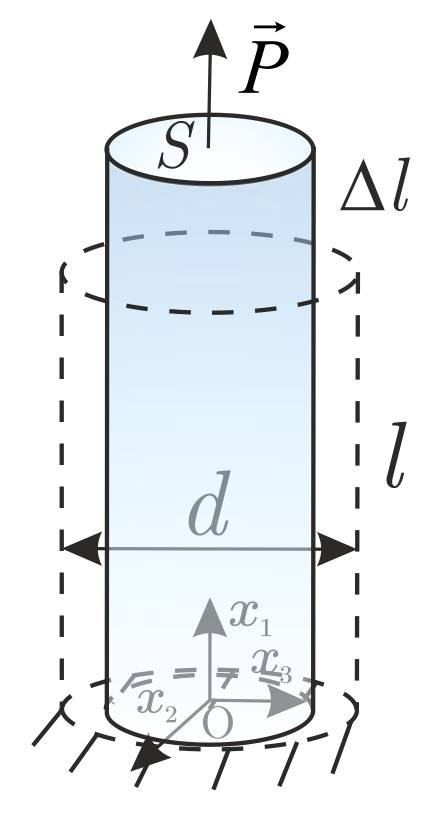
\includegraphics[width=0.3\textwidth]{images/12.2.jpg}
\end{figure}



Экспериментальный закон Гука: при одноосном растяжении призматического тела относ ное удлинение пропорционально приложенной силе на единицу площади $P / S=E \cdot \Delta l / l$, $E$ --- модуль Юнга, $\sigma_{11} \approx P / S \equiv p$ --- напряжение, $\varepsilon_{11} \approx \Delta l / l$ --- деформация $\Rightarrow \sigma_{11}=E \varepsilon_{11}$. 

Экспериментальный закон Пуассона: продольное растяжении приводит к равномерному поперечному сжатию $\Delta d / d=-v \cdot \Delta l / l \Rightarrow \varepsilon_{22}=\varepsilon_{33}=-v \varepsilon_{11}.$ Коэффициент Пуассона - $v$. 
 

Рассмотрим обратный закон Гука и выразим его уравнения через технические константы.
$$
\begin{aligned}
& \begin{array}{c}
\sigma_{i j}=p \delta_{1 i} \delta_{1 j} \\
\sigma=p / 3
\end{array} \Rightarrow \varepsilon_{i j}=-\frac{3 \lambda}{2 \mu(3 \lambda+2 \mu)} \sigma \delta_{i j}+\frac{1}{2 \mu} \sigma_{i j}=\left(-\frac{\lambda}{2 \mu(3 \lambda+2 \mu)} \delta_{i j}+\frac{1}{2 \mu} \delta_{1 i} \delta_{1 j}\right) p \\
& \varepsilon_{11}=\left(-\frac{\lambda}{2 \mu(3 \lambda+2 \mu)}+\frac{1}{2 \mu}\right) p=\frac{\lambda+\mu}{\mu(3 \lambda+2 \mu)} p \Rightarrow E=\frac{\mu(3 \lambda+2 \mu)}{\lambda+\mu} \\
& \begin{array}{l}
\varepsilon_{22} =
\varepsilon_{33}
=\end{array} \frac{-\lambda}{2 \mu(3 \lambda+2 \mu)} p=\frac{-\lambda}{2 \mu(3 \lambda+2 \mu)}\left(E \varepsilon_{11}\right)=\frac{-\lambda}{2(\lambda+\mu)} \varepsilon_{11} \Rightarrow v=\frac{\lambda}{2(\lambda+\mu)} 
\end{aligned}
$$
Выразим коэффициенты Ламе через технические константы.
$$
\begin{aligned}
& \begin{array}{c}
1-2 v=\mu /(\lambda+\mu) \\
1+v=(3 \lambda+2 \mu) / 2(\lambda+\mu)
\end{array} \Rightarrow \frac{E v}{(1-2 v)(1+v)}= \\& =\frac{\mu(3 \lambda+2 \mu)}{\lambda+\mu} \cdot \frac{\lambda}{2(\lambda+\mu)} \cdot \frac{\lambda+\mu}{\mu} \cdot \frac{2(\lambda+\mu)}{3 \lambda+2 \mu}=\lambda \\
& \frac{E}{2(1+v)}=\frac{\mu(3 \lambda+2 \mu)}{\lambda+\mu} \cdot \frac{\lambda+\mu}{3 \lambda+2 \mu}=\mu, \quad \frac{E}{3(1-2 v)}=\frac{\mu(3 \lambda+2 \mu)}{\lambda+\mu} \cdot \frac{\lambda+\mu}{3 \mu}=\lambda+\frac{2}{3} \mu=K \\
& E=\frac{\mu(3 \lambda+2 \mu)}{\lambda+\mu}, \quad v=\frac{\lambda}{2(\lambda+\mu)}, \quad \lambda=\frac{E v}{(1-2 v)(1+v)}, \quad G=\mu=\frac{E}{2(1+v)}, \\ & \quad K=\frac{E}{3(1-2 v)}
\end{aligned}
$$


$\Rightarrow\text{(из критерия Сельвестра)} -1<v<0.5 \text{ и } E>0 $

\vfill


\section{Общая постановка статической краевой задачи теории упругости при малых деформациях и малых поворотах: неизменность геометрической области, занятой деформируемым телом; система пятнадцати уравнений во внутренних точках области; объяснить необходимость условий Сен-Венана; три типа краевых условий. Принцип суперпозиции линейных задач. Теорема единственности решения статической задачи. Постановка задачи теории упругости в перемещениях. Уравнение Ламе.}


В случае малых деформаций и малых вращений элементарные отрезки до и после деформирования различаются мало и по длине и по направлению: $d \vec{r} \approx d \vec{R}$. Следовательно, отсчетная конфигурация тела и его актуальная конфигурация практически совпадают, и в этом случае пропадает разница между Лагранжевыми и Эйлеровыми координатами, т.е. $x_i \approx X_i$. Пропадает разница $\partial / \partial x_i \approx \partial / \partial X_i$ между пространственными и материальными градиентами и между тензорами Грина, Альманси и Коши: $A_{i j} \approx \Gamma_{i j} \approx \varepsilon_{i j}=1 / 2\left(u_{j, i}+u_{i, j}\right)$. При этом вектор перемещений в многих случаях теряет физический смысл и его рассматривают лишь как векторное поле, определенное в трехмерном евклидовом пространстве.

\begin{figure}[h!]
  \centering
  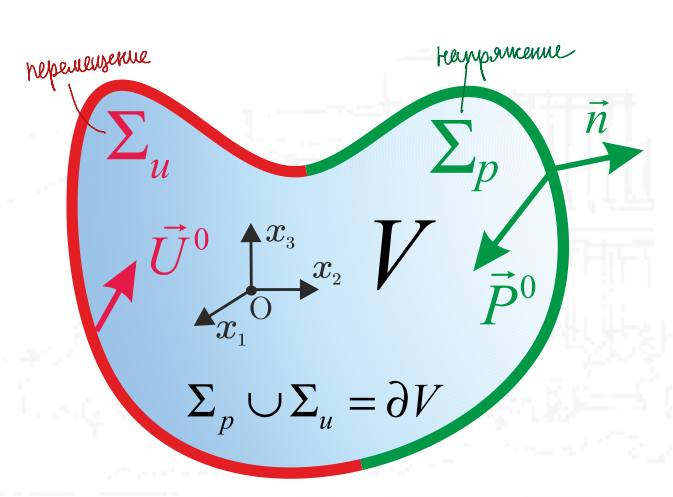
\includegraphics[width=0.5\textwidth]{images/13.1.jpg}
\end{figure}



Упругое равновесие изотропного тела описывается системой 15-ти уравнений на 15-ть функций:


$\begin{aligned} & \left.\sigma_{i j} n_j\right|_{\vec{y} \in \Sigma_p}=P_i^0(\vec{y})  \text{ -- условия Неймана} \\ &
 \sigma_{i j, j}=-\rho F_i \text{ -- уравнения равновесия} \\ &
\sigma_{i j}=\lambda \varepsilon_{k k} \delta_{i j}+2 \mu \varepsilon_{i j} \text{ --  закон Гука} \\ & 
\left.u_i\right|_{\vec{y} \in \Sigma_u}=U_i^0(\vec{y}) \text{ -- условия Дирихле} \\ &
 \varepsilon_{i j}=\Delta_{i j k l} u_{l, k} \text{ -- уравнения Коши}  \\ &
 e_{i k l} e_{j p q} \varepsilon_{k p, l q}=0 \text{ -- уравнения Сен-Венана}\\ &
 i, j=1,2,3 
 \end{aligned}$


\textbf{Необходимость условий Сен-Венана}:
Пусть известны шесть компонент $\varepsilon_{ij}$ тензора деформаций. Требуется по этим компонентам найти три $u_{i}$
непрерывные компоненты вектора перемещений. Формулы компонент тензора Коши можно считать
системой из шести дифференциальных уравнений в частных производных относительно трех компонент
вектора перемещений. Уравнений больше чем неизвестных, поэтому решение может не существовать
(система переопределена). Требуются дополнительные условия на компоненты тензора Коши, которые
гарантируют существование вектора перемещения. Таким условием является в частности формула Чезаро:


$ \displaystyle
u_i^P=u_i^O+\omega_{j i}^O\left(x_j^P-x_j^O\right)+\int_O^P\left[\varepsilon_{i j}+\left(x_k^P-x_k\right)\left(\varepsilon_{i j, k}-\varepsilon_{j k, i}\right)\right] d x_j.
$


 Обозначим $\Psi_{i j}=\varepsilon_{i j}+\left(x_k^P-x_k\right)\left(\varepsilon_{i j, k}-\varepsilon_{j k, i}\right)$. Для того, чтобы $\vec{u}$ было векторным полем значение интеграла в формулах Чезаро не должно зависеть от выбора пути интегрирования, а зависит только от выбора точек начальной и конечной точек (O и Р), т.е: $\oint \Psi_{i j} d x_j=0 \Leftrightarrow \Psi_{i j, l}=\Psi_{i l,j}$
$$
\begin{aligned}
& \left(\varepsilon_{i j}+\left(x_k^P-x_k\right)\left(\varepsilon_{i j, k}-\varepsilon_{j k, i}\right)\right)_{, l}=\left(\varepsilon_{i l}+\left(x_k^P-x_k\right)\left(\varepsilon_{i l, k}-\varepsilon_{l k, i}\right)\right)_{, j} \\
& \varepsilon_{i j, l}-x_{k, l}\left(\varepsilon_{i j, k}-\varepsilon_{j k, i}\right)+\left(x_k^P-x_k\right)\left(\varepsilon_{i j, k l}-\varepsilon_{j k, i l}\right)=\varepsilon_{i l, j}-x_{k, j}\left(\varepsilon_{i l, k}-\varepsilon_{l k, i}\right)+ \\ & +\left(x_k^P-x_k\right)\left(\varepsilon_{i l, k j}-\varepsilon_{l k, i j}\right) \\
& \left(x_k^P-x_k\right)\left(\varepsilon_{i j, k l}-\varepsilon_{j k, i l}-\varepsilon_{i l, k j}+\varepsilon_{l k, i j}\right)=\varepsilon_{i l, j}-\delta_{k j}\left(\varepsilon_{i l, k}-\varepsilon_{l k, i}\right)-\varepsilon_{i j, l}+\delta_{k l}\left(\varepsilon_{i j, k}-\varepsilon_{j k, i}\right) \\
& \left(x_k^P-x_k\right)\left(\varepsilon_{i j, k l}-\varepsilon_{j k, i l}-\varepsilon_{i l, k j}+\varepsilon_{l k, i j}\right)=\varepsilon_{i l, j}-\varepsilon_{i l, j}+\varepsilon_{l j, i}-\varepsilon_{i j, l}+\varepsilon_{i j, l}-\varepsilon_{j l, i}=0 \\
& \text { Получаем } 81 \text { формулу: } \quad \varepsilon_{i j, k l}-\varepsilon_{j k, i l}-\varepsilon_{i l, k j}+\varepsilon_{l k, i j}=0, i, j, k, l=1,2,3.
\end{aligned}
$$


Обозначим $\chi_{i j k l} \equiv \varepsilon_{i j, k l}-\varepsilon_{j k, i l}-\varepsilon_{i l, k j}+\varepsilon_{l k, i j}$ и определим его независимые компоненты. Переставляя индексы исходя из симметрии, получаем 6 езависимых компонент: $\chi_{\underline{1} \underline{12} 2}, \chi_{\underline{1} 123}, \chi_{\underline{1} 1 \underline{3} 3}, \chi_{\underline{1} 2 \underline{2} 3}, \chi_{\underline{2} 2 \underline{3} 3}, \chi_{\underline{1} 2 \underline{3} 3}$.
Соотношения
(уравнения)
Сен-Венана:
$$
\left\{\begin{array}{l}
\varepsilon_{11,22}+\varepsilon_{22,11}=2 \varepsilon_{12,12} \\
\varepsilon_{11,33}+\varepsilon_{33,11}=2 \varepsilon_{13,13} \\
\varepsilon_{22,33}+\varepsilon_{33,22}=2 \varepsilon_{23,23}
\end{array} ;\left\{\begin{array}{l}
\left(\varepsilon_{12,3}-\varepsilon_{23,1}+\varepsilon_{31,2}\right)_{, 1}=\varepsilon_{11,23} \\
\left(\varepsilon_{12,3}+\varepsilon_{23,1}-\varepsilon_{31,2}\right)_{, 2}=\varepsilon_{22,13} \\
\left(-\varepsilon_{12,3}+\varepsilon_{23,1}+\varepsilon_{31,2}\right)_{, 3}=\varepsilon_{33,12}
\end{array}\right.\right.
$$

\textbf{3 типа краевых условий:}


\underline{Первая краевая задача (задача Дирихле, задача в перемещениях)}

\begin{figure}[h!]
  \centering
  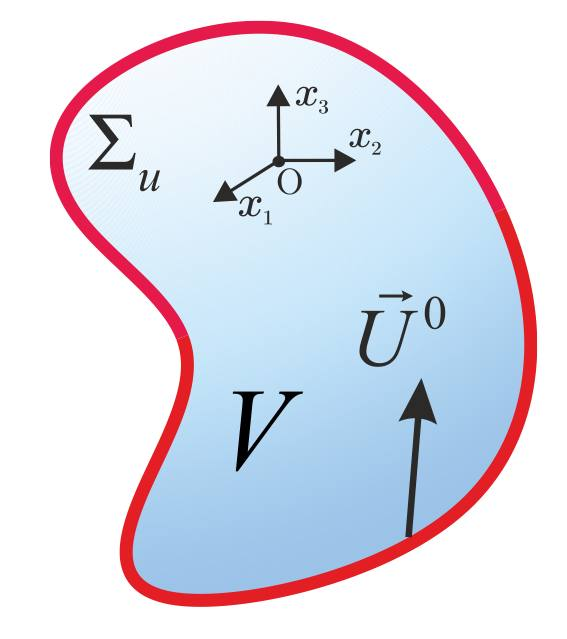
\includegraphics[width=0.3\textwidth]{images/13.2.jpg}
\end{figure}



На границе тела заданы перемещения. Для однородного материала:
$$\displaystyle
\begin{aligned} & \left\{\begin{array}{l}(\lambda+\mu) \mathrm{grad} \mathrm{div} \overrightarrow{\mathrm{u}}+\mu \Delta \overrightarrow{\mathrm{u}}+\rho \vec{F}=\overrightarrow{0} \\ \left.u_i(\vec{y})\right|_{\vec{y} \in \partial V}=U_i^0(\vec{y}), i=1,2,3, \vec{x} \in V\end{array}\right. \Rightarrow \left\{\begin{array}{l}(\lambda+\mu) u_{j, j i}(\vec{x})+\mu u_{i, j j}(\vec{x})=-\rho F_i(\vec{x}) \\ \left.u_i(\vec{y})\right|_{\vec{y} \in \partial V}=U_i^0(\vec{y}), \quad i=1,2,3, \quad \vec{x} \in V\end{array}\right.\end{aligned}$$

 
После того, как найден вектор перемещений, по формулам Коши находим тензор деформаций:
$$
\begin{aligned}
\underset{\sim}{\varepsilon} & =\tenq{\Delta} \cdot\cdot(\vec{\nabla} \otimes \overrightarrow{\mathbf{u}}) \Rightarrow
\varepsilon_{i j} & =\frac{1}{2}\left(u_{j, i}+u_{i, j}\right)
\end{aligned}
$$


Определяем тензор напряжений с помощью закона Гука:
$$
\begin{aligned}
& \underset{\sim}{\sigma}=(\lambda \underset{\sim}{g} \otimes \underset{\sim}{g}+2 \mu \tenq{\Delta}) \cdot \underset{\sim}{\varepsilon} \Rightarrow
& \sigma_{i j}=\lambda \varepsilon_{k k} \delta_{i j}+2 \mu \varepsilon_{i j}
\end{aligned}
$$


\underline{Вторая задача (задача Нейнмана, задача в напряжениях)}

\begin{figure}[h!]
  \centering
  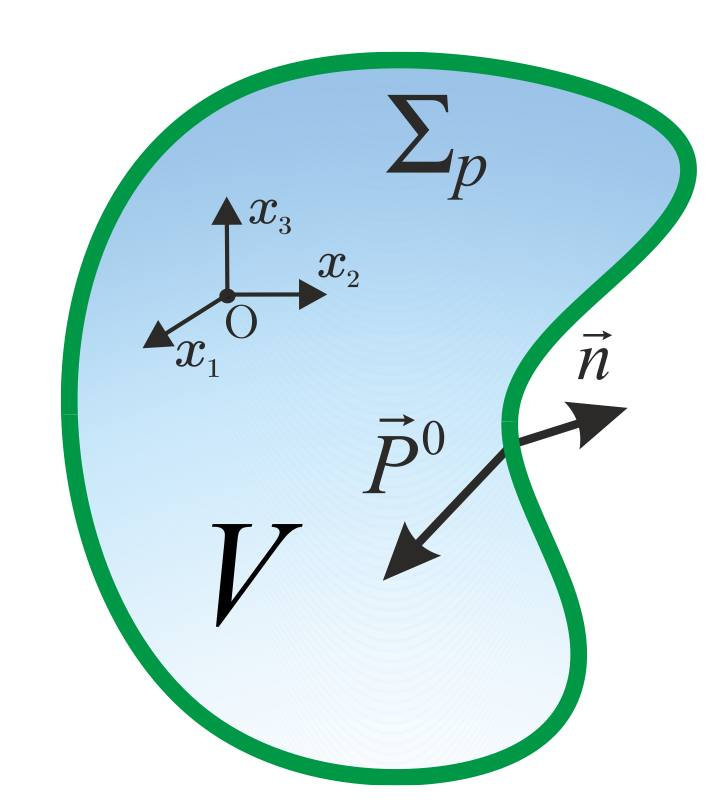
\includegraphics[width=0.3\textwidth]{images/13.3.jpg}
\end{figure}




На границе тела заданы напряжения, 6 функций. Для однородного материала:
$$
\begin{aligned}
& \frac{1+v}{3} \Delta \sigma_{33}+\sigma_{, 33}=-\frac{2(1+v)}{3} \rho F_{3,3}-\frac{v(1+v)}{3(1-v)} \rho F_{k, k} \\
& \frac{1+v}{3} \Delta \sigma_{23}+\sigma_{23}=-\frac{1+v}{3} \rho\left(F_{2,3}+F_{3,2}\right) \\
& \frac{1+v}{3} \Delta \sigma_{13}+\sigma_{, 13}=-\frac{1+v}{3} \rho\left(F_{1,3}+F_{3,1}\right) \\
& \frac{1+v}{3} \Delta \sigma_{22}+\sigma_{, 22}=-\frac{2(1+v)}{3} \rho F_{2,2}-\frac{v(1+v)}{3(1-v)} \rho F_{k, k} \\
& \frac{1+v}{3} \Delta \sigma_{11}+\sigma_{, 11}=-\frac{2(1+v)}{3} \rho F_{1,1}-\frac{v(1+v)}{3(1-v)} \rho F_{k, k} \\
& \frac{1+v}{3} \Delta \sigma_{12}+\sigma_{, 12}=-\frac{1+v}{3} \rho\left(F_{1,2}+F_{2,1}\right) \\
& \left.\sigma_{i j} n_j\right|_{\bar{y} \in \partial V}=P_i^0(\vec{y}), \quad \sigma_{i j, j}=-\rho F_i, \quad \vec{x} \in V 
\end{aligned}
$$
Из обратного закона Гука вычисляем тензор деформаций:
$$
\begin{aligned}
& \underset{\sim}{\varepsilon}=\left(-\frac{v}{E} \underset{\sim}{\mathbf{g}} \otimes \underset{\sim}{\mathbf{g}}+\frac{1+v}{E} \tenq{\Delta}\right) \cdot\cdot \underset{\sim}{\sigma}  \Rightarrow
& \varepsilon_{i j}=-\frac{3 v}{E} \sigma \delta_{i j}+\frac{1+v}{E} \sigma_{i j} 
\end{aligned}
$$
Находим вектор перемещения с помощью формул Чезаро:
$$
u_i^P=u_i^O+\omega_{j i}^O\left(x_j^P-x_j^O\right)+\int_0^P\left[\varepsilon_{i j}+\left(x_k^P-x_k\right)\left(\varepsilon_{i j, k}-\varepsilon_{j k, i}\right)\right] d x_j.
$$
\underline{Смешанная краевая задача}

Частично задаются напряжения и премещения (см. полуобратный метод Сен-Венана), комбинация 1 и 2 задач.


Из линейности этих уравнений описывающих граничные услови я по напряжениям, деформациям и перемещениям следует \textbf{принцип суперпозиции линейных задач} --- возможность наложения  различных решений системы уравнений при условии, что их сумма удовлетворяет граничным условиям. 
(Принцип суперпозиции позволяет выделить четыре основные задачи: о растяжении, чистом изгибе, о кручении и об изгибе силой.)


\textbf{Теорема о единственности решения краевой статической задачи}


Докажем, что однородная статическая задача в отсутствии массовых сил имеет единственное решение.


$$
\begin{aligned}
& \begin{array}{ccc}
\sigma_{i j, j}=0, \quad \sigma_{i j}=\lambda \varepsilon_{k k} \delta_{i j}+2 \mu \varepsilon_{i j} & \left.\sigma_{i j} n_j\right|_{\vec{y} \in \Sigma_p}=0 \\
\varepsilon_{i j}=\Delta_{i j k l} u_{l, k}, \quad e_{i k l} e_{j p q} \varepsilon_{k p, l q}=0 & \left.u_i\right|_{\vec{y} \in \Sigma_u}=0
\end{array} 
\end{aligned}$$

Преобразуем уравнения равновесия, свернув его с вектором перемещения. Результат проинтегрируем по всему телу: 
$ 
\displaystyle
0=\sigma_{i j, j} u_i=\left(\sigma_{i j} u_i\right)_{, j}-\sigma_{i j} u_{i, j}=\left(\sigma_{i j} u_i\right)_{, j}-\sigma_{i j} \varepsilon_{i j} \Rightarrow 0=\int_V\left(\left(\sigma_{i j} u_i\right)_{, j}-\sigma_{i j} \varepsilon_{i j}\right) d \vec{x}=\int_V\left(\sigma_{i j} u_i\right)_{, j} d \vec{x}-\int_V \sigma_{i j} \varepsilon_{i j} d \vec{x}=\int_{\partial V} \sigma_{i j} u_i n_j d \Sigma-\int_V \sigma_{i j} \varepsilon_{i j} d \vec{x}=\int_{\Sigma_p} \sigma_{i j} u_i n_j d \Sigma+ \int_{\Sigma_u} \sigma_{i j} u_i n_j d \Sigma- \int_V \sigma_{i j} \varepsilon_{i j} d \vec{x}=\int_{\Sigma_p} P_i^0 u_i d \Sigma+\int_{\Sigma_u} \sigma_{i j} n_j u_i d \Sigma-\int_V \sigma_{i j} \varepsilon_{i j} d \vec{x}=-\int_V \sigma_{i j} \varepsilon_{i j} d \vec{x} \Rightarrow  \int_V \sigma_{i j} \varepsilon_{i j} d \vec{x}=\int_V\left(K \theta^2+G \Gamma^2\right) d \vec{x}=0 \Rightarrow\left\{\begin{array}{l}
\theta=0 \Rightarrow \varepsilon_{i j}=e_{i j} \\
\Gamma=0 \Rightarrow e_{i j} \equiv 0
\end{array} \Rightarrow \varepsilon_{i j} \equiv 0\right.
$

Из формул Чезаро получаем $u_i=u_i^0+\omega_{j i}^0\left(x_j-x_j^0\right)$. 


Из закона Гука получаем $\sigma_{i j}=C_{i j k l} \varepsilon_{k l} \equiv 0$.
Вывод: решением однородной статической краевой задачи упругости является движение абсолютно твердого тела (перемещение и вращение). 


Теперь рассмотрим неоднородную задачу и предположим, что существует два различных решения: $\left(\underset{\sim}{\boldsymbol{\varepsilon}^{\prime}}, \underset{\sim}{\boldsymbol{\sigma}^{\prime}}, \vec{u}^{\prime}\right)$ и $\left(\underset{\sim}{\boldsymbol{\varepsilon^{\prime\prime}}}, \underset{\sim}{\boldsymbol{\sigma}^{\prime \prime}}, \vec{u}^{\prime \prime}\right)$. Рассмотрим разность этих двух задач:
$$
\left\{\begin{array}{l}
\sigma_{i j, j}^{\prime}=-\rho F_i \\
\sigma_{i j}^{\prime}=\lambda \theta^{\prime} \delta_{i j}+2 \mu \varepsilon_{i j}^{\prime} \\
e_{i k l} e_{j p q} \varepsilon_{k p, l q}^{\prime}=0 \\
\varepsilon_{i j}^{\prime}=\Delta_{i j k l} u_{l, k}^{\prime} \\
\left.\sigma_{i j}^{\prime} n_j\right|_{\vec{y} \in \Sigma_p}=P_i^0 \\
\left.u_i^{\prime}\right|_{\bar{y} \in \Sigma_u}=U_i^0
\end{array} \quad-\left\{\begin{array}{l}
\sigma_{i j, j}^{\prime \prime}=-\rho F_i \\
\sigma_{i j}^{\prime \prime}=\lambda \theta^{\prime \prime} \delta_{i j}+2 \mu \varepsilon_{i j}^{\prime \prime} \\
e_{i k l} e_{j p q} \varepsilon_{k p, l q}^{\prime \prime}=0 \\
\varepsilon_{i j}^{\prime \prime}=\Delta_{i j k l} u_{l, k}^{\prime \prime} \\
\left.\sigma_{i j}^{\prime \prime} n_j\right|_{\bar{y} \in \Sigma_p}=P_i^0 \\
\left.u_i^{\prime \prime}\right|_{\bar{y} \in \Sigma_u}=U_i^0
\end{array}=\right.\right.
\left\{\begin{array}{l}
\left(\sigma_{i j}^{\prime}-\sigma_{i j}^{\prime \prime}\right)_{, j}=0 \\
\left(\sigma_{i j}^{\prime}-\sigma_{i j}^{\prime \prime}\right)=\lambda\left(\theta^{\prime}-\theta^{\prime \prime}\right) \delta_{i j}+\\
+2 \mu\left(\varepsilon_{i j}^{\prime}-\varepsilon_{i j}^{\prime \prime}\right)\\
e_{i k l} e_{j p q}\left(\varepsilon_{k p}^{\prime}-\varepsilon_{k p}^{\prime \prime}\right)_{, l q}=0 \\
\left(\varepsilon_{i j}^{\prime}-\varepsilon_{i j}^{\prime \prime}\right)=\Delta_{i j k l}\left(u_l^{\prime}-u_i^{\prime}\right. \\
\left.\left(\sigma_{i j}^{\prime}-\sigma_{i j}^{\prime \prime}\right) n_j\right|_{\bar{y} \in \Sigma_p}=0 \\
\left.\left(u_i^{\prime}-u_i^{\prime \prime}\right)\right|_{\bar{y} \in \Sigma_u}=0
\end{array}\right.
$$
Два решения отличаются на движение абсолютно твёрдого тела: $\left(\underset{\sim}\varepsilon^\prime-{\underset{\sim}{\boldsymbol{\varepsilon}}}^{\prime \prime}, \underset{\sim}{\boldsymbol{\sigma}}-{\underset{\sim}{\boldsymbol{\sigma}}}^{\prime \prime}, \vec{u}^{\prime}-\vec{u}^{\prime \prime}\right)$


Для исследования свойств системы уравнений равновесия и получения аналитических решений можно исключить из системы уравнений компоненты напряжения и деформации с помощью закона Гука и кинематических соотношений, тогда получаются \textbf{уравнения в перемещениях} (см. первую краевую задачу). Деформации и напряжения определяются по ним. Можно не рассматривать перемещения, а только условия совместности, закон Гука и уравнения равновесия, тогда можно получить\textbf{уравнения в напряжениях} (см. вторую краевую задачу).


\textbf{Уравнение Ламе}


Подставим уравнения Коши в закон Гука (для изотропной однородной среды) и полученный результат подставим в уравнения движения:


$ \displaystyle
\underset{\sim}{\boldsymbol{\sigma}}=(\lambda \underset{\sim}{\mathbf{g}} \otimes \underset{\sim}{\mathbf{g}}+2 \mu \tenq{\mathbf{\Delta}}) \cdot\cdot \underset{\sim}{\boldsymbol{\varepsilon}}=\lambda \underset{\sim}{\mathbf{g}} \otimes \underset{\sim}{\mathbf{g}} \cdot\cdot \underset{\sim}{\boldsymbol{\varepsilon}}+2 \mu \underset{\sim}{\mathbf{D^S}}=\lambda \underset{\sim}{\mathbf{g}} \theta+\mu \underset{\sim}{\mathrm{D^T}}+\mu \underset{\sim}{\mathbf{D}} \Rightarrow \vec{\nabla} \cdot \underset{\sim}{\sigma}=\lambda \vec{\nabla} \otimes \theta+\mu \vec{\nabla} \cdot(\overrightarrow{\mathrm{u}} \otimes \vec{\nabla})
+\mu \vec{\nabla} \cdot(\vec{\nabla} \otimes \overrightarrow{\mathrm{u}})=\lambda \vec{\nabla} \otimes \theta+\mu \theta \otimes \vec{\nabla}+\mu \Delta \overrightarrow{\mathrm{u}}=(\lambda+\mu) \vec{\nabla} \theta+\mu \Delta \overrightarrow{\mathrm{u}}=(\lambda+\mu) \mathrm{grad} \mathrm{div} \overrightarrow{\mathrm{u}}+\mu \Delta \overrightarrow{\mathrm{u}} $
$$
(\lambda+\mu) \mathrm{grad} \mathrm{div} \overrightarrow{\mathrm{u}}+\mu \Delta \overrightarrow{\mathrm{u}}+\rho \vec{F}=\rho \frac{\partial^2 \overrightarrow{\mathrm{u}}}{\partial t^2}
$$
Уравнения Ламе в координатной форме (порядок индексов несущественен):


В декартовых координатах:
$(\lambda+\mu) \frac{\partial^2 u_\alpha}{\partial x_\alpha \partial x_i}+\mu \frac{\partial^2 u_i}{\partial x_\alpha \partial x_\alpha}+\rho F_i=\rho \frac{\partial^2 u_i}{\partial t^2}, i=1,2,3$.


Разделение на потенциальные:
$$(\lambda+2 \mu) \mathrm{grad} \mathrm{div} \overrightarrow{\mathrm{u}}-\mathrm{rot} \mathrm{rot} \overrightarrow{\mathrm{u}}+\rho \vec{F}=\rho \partial^2 \overrightarrow{\mathrm{u}} / \partial t^2$$
и вихревые слагаемые:
$$
(\lambda+2 \mu) u_{\alpha \beta}^\alpha g^{i \beta}-\mu(\mathrm{rot} \mathrm{rot} \vec{u})^i+\rho F^i=\rho \partial^2 u^i / \partial t^2, i=1,2,3 \text {. }
$$
уравнение равновесия Ламе: $(\lambda+\mu) \mathrm{grad} \mathrm{div} \overrightarrow{\mathrm{u}}+\mu \Delta \overrightarrow{\mathrm{u}}+\rho \vec{F}=\overrightarrow{0}$



\section{Общая постановка статической краевой задачи теории упругости при малых деформациях и малых поворотах: неизменность геометрической области, занятой деформируемым телом; система пятнадцати уравнений во внутренних точках области; объяснить необходимость условий Сен-Венана; три типа краевых условий. Постановка задачи теории упругости в напряжениях. Уравнения Бельтрами-Митчелла.}


В случае малых деформаций и малых вращений элементарные отрезки до и после деформирования различаются мало и по длине и по направлению: $d \vec{r} \approx d \vec{R}$. Следовательно, отсчетная конфигурация тела и его актуальная конфигурация практически совпадают, и в этом случае пропадает разница между Лагранжевыми и Эйлеровыми координатами, т.е. $x_i \approx X_i$. Пропадает разница $\partial / \partial x_i \approx \partial / \partial X_i$ между пространственными и материальными градиентами и между тензорами Грина, Альманси и Коши: $A_{i j} \approx \Gamma_{i j} \approx \varepsilon_{i j}=1 / 2\left(u_{j, i}+u_{i, j}\right)$. При этом вектор перемещений в многих случаях теряет физический смысл и его рассматривают лишь как векторное поле, определенное в трехмерном евклидовом пространстве.

\begin{figure}[h!]
  \centering
  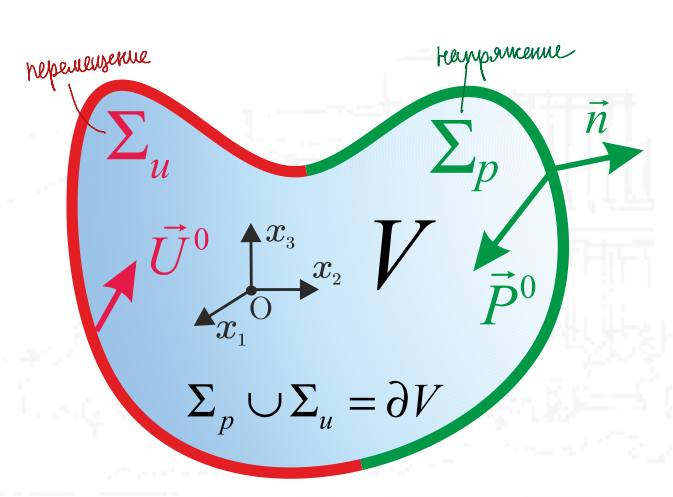
\includegraphics[width=0.3\textwidth]{images/13.1.jpg}
\end{figure}



Упругое равновесие изотропного тела описывается системой 15-ти уравнений на 15-ть функций:


$\begin{aligned} & \left.\sigma_{i j} n_j\right|_{\vec{y} \in \Sigma_p}=P_i^0(\vec{y})  \text{ -- условия Неймана} \\ &
 \sigma_{i j, j}=-\rho F_i \text{ -- уравнения равновесия} \\ &
\sigma_{i j}=\lambda \varepsilon_{k k} \delta_{i j}+2 \mu \varepsilon_{i j} \text{ --  закон Гука} \\ & 
\left.u_i\right|_{\vec{y} \in \Sigma_u}=U_i^0(\vec{y}) \text{ -- условия Дирихле} \\ &
 \varepsilon_{i j}=\Delta_{i j k l} u_{l, k} \text{ -- уравнения Коши}  \\ &
 e_{i k l} e_{j p q} \varepsilon_{k p, l q}=0 \text{ -- уравнения Сен-Венана}\\ &
 i, j=1,2,3 
 \end{aligned}$


\textbf{Необходимость условий Сен-Венана}:
Пусть известны шесть компонент $\varepsilon_{ij}$ тензора деформаций. Требуется по этим компонентам найти три $u_{i}$
непрерывные компоненты вектора перемещений. Формулы компонент тензора Коши можно считать
системой из шести дифференциальных уравнений в частных производных относительно трех компонент
вектора перемещений. Уравнений больше чем неизвестных, поэтому решение может не существовать
(система переопределена). Требуются дополнительные условия на компоненты тензора Коши, которые
гарантируют существование вектора перемещения. Таким условием является в частности формула Чезаро:


$ \displaystyle
u_i^P=u_i^O+\omega_{j i}^O\left(x_j^P-x_j^O\right)+\int_O^P\left[\varepsilon_{i j}+\left(x_k^P-x_k\right)\left(\varepsilon_{i j, k}-\varepsilon_{j k, i}\right)\right] d x_j.
$


 Обозначим $\Psi_{i j}=\varepsilon_{i j}+\left(x_k^P-x_k\right)\left(\varepsilon_{i j, k}-\varepsilon_{j k, i}\right)$. Для того, чтобы $\vec{u}$ было векторным полем значение интеграла в формулах Чезаро не должно зависеть от выбора пути интегрирования, а зависит только от выбора точек начальной и конечной точек (O и Р), т.е: $\oint \Psi_{i j} d x_j=0 \Leftrightarrow \Psi_{i j, l}=\Psi_{i l,j}$
$$
\begin{aligned}
& \left(\varepsilon_{i j}+\left(x_k^P-x_k\right)\left(\varepsilon_{i j, k}-\varepsilon_{j k, i}\right)\right)_{, l}=\left(\varepsilon_{i l}+\left(x_k^P-x_k\right)\left(\varepsilon_{i l, k}-\varepsilon_{l k, i}\right)\right)_{, j} \\
& \varepsilon_{i j, l}-x_{k, l}\left(\varepsilon_{i j, k}-\varepsilon_{j k, i}\right)+\left(x_k^P-x_k\right)\left(\varepsilon_{i j, k l}-\varepsilon_{j k, i l}\right)=\varepsilon_{i l, j}-x_{k, j}\left(\varepsilon_{i l, k}-\varepsilon_{l k, i}\right)+\\ &+\left(x_k^P-x_k\right)\left(\varepsilon_{i l, k j}-\varepsilon_{l k, i j}\right) \\
& \left(x_k^P-x_k\right)\left(\varepsilon_{i j, k l}-\varepsilon_{j k, i l}-\varepsilon_{i l, k j}+\varepsilon_{l k, i j}\right)=\varepsilon_{i l, j}-\delta_{k j}\left(\varepsilon_{i l, k}-\varepsilon_{l k, i}\right)-\varepsilon_{i j, l}+\delta_{k l}\left(\varepsilon_{i j, k}-\varepsilon_{j k, i}\right) \\
& \left(x_k^P-x_k\right)\left(\varepsilon_{i j, k l}-\varepsilon_{j k, i l}-\varepsilon_{i l, k j}+\varepsilon_{l k, i j}\right)=\varepsilon_{i l, j}-\varepsilon_{i l, j}+\varepsilon_{l j, i}-\varepsilon_{i j, l}+\varepsilon_{i j, l}-\varepsilon_{j l, i}=0 \\
& \text { Получаем } 81 \text { формулу: } \quad \varepsilon_{i j, k l}-\varepsilon_{j k, i l}-\varepsilon_{i l, k j}+\varepsilon_{l k, i j}=0, i, j, k, l=1,2,3.
\end{aligned}
$$


Обозначим $\chi_{i j k l} \equiv \varepsilon_{i j, k l}-\varepsilon_{j k, i l}-\varepsilon_{i l, k j}+\varepsilon_{l k, i j}$ и определим его независимые компоненты. Переставляя индексы исходя из симметрии, получаем 6 езависимых компонент: $\chi_{\underline{1} \underline{12} 2}, \chi_{\underline{1} 123}, \chi_{\underline{1} 1 \underline{3} 3}, \chi_{\underline{1} 2 \underline{2} 3}, \chi_{\underline{2} 2 \underline{3} 3}, \chi_{\underline{1} 2 \underline{3} 3}$.
Соотношения
(уравнения)
Сен-Венана:
$$
\left\{\begin{array}{l}
\varepsilon_{11,22}+\varepsilon_{22,11}=2 \varepsilon_{12,12} \\
\varepsilon_{11,33}+\varepsilon_{33,11}=2 \varepsilon_{13,13} \\
\varepsilon_{22,33}+\varepsilon_{33,22}=2 \varepsilon_{23,23}
\end{array} ;\left\{\begin{array}{l}
\left(\varepsilon_{12,3}-\varepsilon_{23,1}+\varepsilon_{31,2}\right)_{, 1}=\varepsilon_{11,23} \\
\left(\varepsilon_{12,3}+\varepsilon_{23,1}-\varepsilon_{31,2}\right)_{, 2}=\varepsilon_{22,13} \\
\left(-\varepsilon_{12,3}+\varepsilon_{23,1}+\varepsilon_{31,2}\right)_{, 3}=\varepsilon_{33,12}
\end{array}\right.\right.
$$

\textbf{3 типа краевых условий:}


\underline{Первая краевая задача (задача Дирихле, задача в перемещениях)}
\begin{figure}[h!]
  \centering
  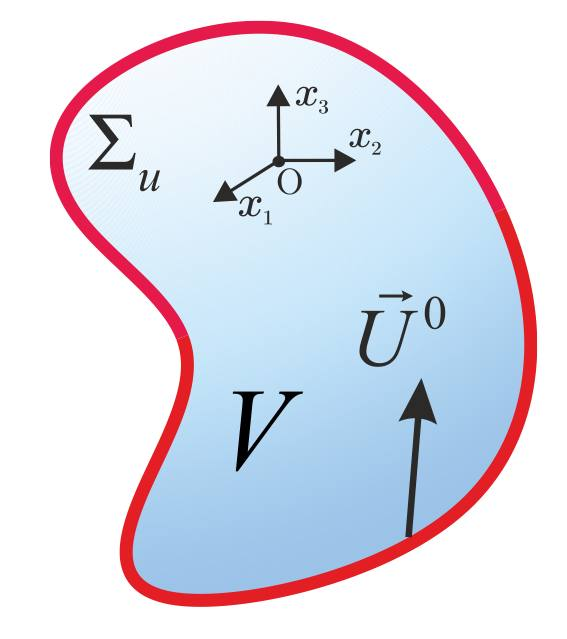
\includegraphics[width=0.3\textwidth]{images/13.2.jpg}
\end{figure}

На границе тела заданы перемещения. Для однородного материала:
$$\displaystyle
\begin{aligned} & \left\{\begin{array}{l}(\lambda+\mu) \mathrm{grad} \mathrm{div} \overrightarrow{\mathrm{u}}+\mu \Delta \overrightarrow{\mathrm{u}}+\rho \vec{F}=\overrightarrow{0} \\ \left.u_i(\vec{y})\right|_{\vec{y} \in \partial V}=U_i^0(\vec{y}), i=1,2,3, \vec{x} \in V\end{array}\right. \Rightarrow \left\{\begin{array}{l}(\lambda+\mu) u_{j, j i}(\vec{x})+\mu u_{i, j j}(\vec{x})=-\rho F_i(\vec{x}) \\ \left.u_i(\vec{y})\right|_{\vec{y} \in \partial V}=U_i^0(\vec{y}), \quad i=1,2,3, \quad \vec{x} \in V\end{array}\right.\end{aligned}$$

 
После того, как найден вектор перемещений, по формулам Коши находим тензор деформаций:
$$
\begin{aligned}
\underset{\sim}{\varepsilon} & =\tenq{\Delta} \cdot\cdot(\vec{\nabla} \otimes \overrightarrow{\mathbf{u}}) \Rightarrow
\varepsilon_{i j} & =\frac{1}{2}\left(u_{j, i}+u_{i, j}\right)
\end{aligned}
$$


Определяем тензор напряжений с помощью закона Гука:
$$
\begin{aligned}
& \underset{\sim}{\sigma}=(\lambda \underset{\sim}{g} \otimes \underset{\sim}{g}+2 \mu \tenq{\Delta}) \cdot \underset{\sim}{\varepsilon} \Rightarrow
& \sigma_{i j}=\lambda \varepsilon_{k k} \delta_{i j}+2 \mu \varepsilon_{i j}
\end{aligned}
$$


\underline{Вторая задача (задача Нейнмана, задача в напряжениях)}

\begin{figure}[h!]
  \centering
  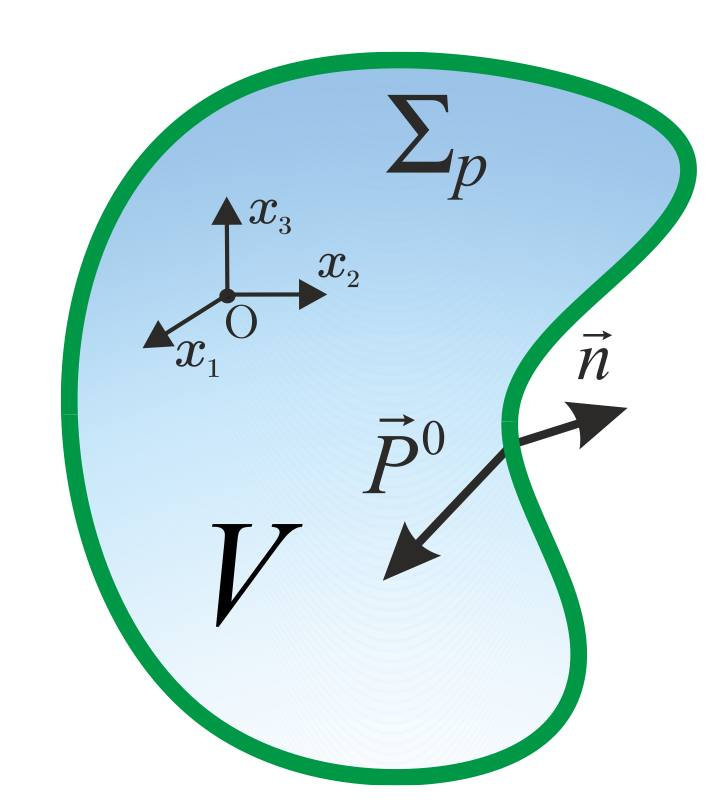
\includegraphics[width=0.3\textwidth]{images/13.3.jpg}
\end{figure}



На границе тела заданы напряжения, 6 функций. Для однородного материала:
$$
\begin{aligned}
& \frac{1+v}{3} \Delta \sigma_{33}+\sigma_{, 33}=-\frac{2(1+v)}{3} \rho F_{3,3}-\frac{v(1+v)}{3(1-v)} \rho F_{k, k} \\
& \frac{1+v}{3} \Delta \sigma_{23}+\sigma_{23}=-\frac{1+v}{3} \rho\left(F_{2,3}+F_{3,2}\right) \\
& \frac{1+v}{3} \Delta \sigma_{13}+\sigma_{, 13}=-\frac{1+v}{3} \rho\left(F_{1,3}+F_{3,1}\right) \\
& \frac{1+v}{3} \Delta \sigma_{22}+\sigma_{, 22}=-\frac{2(1+v)}{3} \rho F_{2,2}-\frac{v(1+v)}{3(1-v)} \rho F_{k, k} \\
& \frac{1+v}{3} \Delta \sigma_{11}+\sigma_{, 11}=-\frac{2(1+v)}{3} \rho F_{1,1}-\frac{v(1+v)}{3(1-v)} \rho F_{k, k} \\
& \frac{1+v}{3} \Delta \sigma_{12}+\sigma_{, 12}=-\frac{1+v}{3} \rho\left(F_{1,2}+F_{2,1}\right) \\
& \left.\sigma_{i j} n_j\right|_{\bar{y} \in \partial V}=P_i^0(\vec{y}), \quad \sigma_{i j, j}=-\rho F_i, \quad \vec{x} \in V 
\end{aligned}
$$
Из обратного закона Гука вычисляем тензор деформаций:
$$
\begin{aligned}
& \underset{\sim}{\varepsilon}=\left(-\frac{v}{E} \underset{\sim}{\mathbf{g}} \otimes \underset{\sim}{\mathbf{g}}+\frac{1+v}{E} \tenq{\Delta}\right) \cdot\cdot \underset{\sim}{\sigma}  \Rightarrow
& \varepsilon_{i j}=-\frac{3 v}{E} \sigma \delta_{i j}+\frac{1+v}{E} \sigma_{i j} 
\end{aligned}
$$
Находим вектор перемещения с помощью формул Чезаро:
$$
u_i^P=u_i^O+\omega_{j i}^O\left(x_j^P-x_j^O\right)+\int_0^P\left[\varepsilon_{i j}+\left(x_k^P-x_k\right)\left(\varepsilon_{i j, k}-\varepsilon_{j k, i}\right)\right] d x_j.
$$
\underline{Смешанная краевая задача}

Частично задаются напряжения и премещения (см. полуобратный метод Сен-Венана), комбинация 1 и 2 задач.


Для исследования свойств системы уравнений равновесия и получения аналитических решений можно исключить из системы уравнений компоненты напряжения и деформации с помощью закона Гука и кинематических соотношений, тогда получаются \textbf{уравнения в перемещениях} (см. первую краевую задачу). Деформации и напряжения определяются по ним. Можно не рассматривать перемещения, а только условия совместности, закон Гука и уравнения равновесия, тогда можно получить\textbf{уравнения в напряжениях} (см. вторую краевую задачу).


\textbf{Уравнения Бельтрама--Митчела}


Уравнения Бельтрами-Митчелла применяют для решения статических задач однородного, изотропного линейно-упругого тела. Получим их подстановкой закона Гука в уравнения совместности и равновесия.
$$
\begin{aligned}
&\left\{\begin{array}{l}
\varepsilon_{11,22}+\varepsilon_{22,11}=2 \varepsilon_{12,12} \\
\varepsilon_{11,33}+\varepsilon_{33,11}=2 \varepsilon_{13,13} \\
\varepsilon_{22,33}+\varepsilon_{33,22}=2 \varepsilon_{23,23}
\end{array} ;\left\{\begin{array}{l}
\left(\varepsilon_{12,3}+\varepsilon_{23,1}+\varepsilon_{31,2}\right)_{, 1}=\varepsilon_{11,23} \\\left(\varepsilon_{12,3}+\varepsilon_{23,1}-\varepsilon_{31,2}\right)_{, 2}=\varepsilon_{22,13} \\
\left(-\varepsilon_{12,3}+\varepsilon_{23,1}+\varepsilon_{31,2}\right)_{, 3}=\varepsilon_{33,12}
\end{array}\right.\right. \\
& \sigma_{i j, j}+\rho F_i=0,\quad i=1,2,3.\quad \varepsilon_{i j}=-\frac{3 v}{E} \sigma \delta_{i j}+\frac{1+v}{E} \sigma_{i j} 
\end{aligned}
$$
Подставим обратный закон Гука в уравнения Сен-Венана. Получим щесть уравнений Сен-Венана, выраженные через компоненты тензора напряжений:
$$
\left\{\begin{array}{l}
\sigma_{11,22}+\sigma_{22,11}-\frac{3 v}{1+v}\left(\sigma_{, 11}+\sigma_{, 22}\right)=2 \sigma_{12,12} \\
\sigma_{11,33}+\sigma_{33,11}-\frac{3 v}{1+v}\left(\sigma_{, 11}+\sigma_{, 33}\right)=2 \sigma_{13,13} \\
\sigma_{22,33}+\sigma_{33,22}-\frac{3 v}{1+v}\left(\sigma_{, 22}+\sigma_{, 33}\right)=2 \sigma_{23,23}
\end{array} ; \begin{cases}\sigma_{11,23}-\frac{3 v}{1+v} \sigma_{, 23}=\left(\sigma_{12,3}-\sigma_{23,1}+\sigma_{31,2}\right)_{, 1} & \\
\sigma_{22,13}-\frac{3 v}{1+v} \sigma_{, 13}=\left(\sigma_{12,3}+\sigma_{23,1}-\sigma_{31,2}\right)_{, 2} &  \\
\sigma_{33,12}-\frac{3 v}{1+v} \sigma_{, 12}=\left(-\sigma_{12,3}+\sigma_{23,1}+\sigma_{31,2}\right)_{, 3} & \end{cases}\right.
$$


Продифференцируем первое уравнение равновесия по $\boldsymbol{x}_1$, второе по $\boldsymbol{x}_2$, третье уравнение по $\boldsymbol{x}_3$. Теперь сложим первых два уравнения и вычтем третье. Повторим операцию ещё 2 раза: сложим первое и третье уравнения и вычтем второе, а затем сложим второе и третье уравнения и вычтем первое:
$$
\begin{aligned}
& \sigma_{11,1}+\sigma_{12,2}+\sigma_{13,3}+\rho F_1=0 \quad \quad \sigma_{11,11}+\sigma_{12,21}+\sigma_{13,31}+\rho F_{1,1}=0 \quad \\
& \sigma_{21,1}+\sigma_{22,2}+\sigma_{23,3}+\rho F_2=0 \Rightarrow \sigma_{21,12}+\sigma_{22,22}+\sigma_{23,32}+\rho F_{2,2}=0 \Rightarrow \\
& \sigma_{31,1}+\sigma_{32,2}+\sigma_{33,3}+\rho F_3=0 \quad \quad \sigma_{31,13}+\sigma_{32,23}+\sigma_{33,33}+\rho F_{3,3}=0 \quad 
\end{aligned}
$$
$$
\begin{aligned}
&\underline{\sigma_{11,11}}+\underline{\underline{\sigma_{22,22}}}-\sigma_{33,33}=\rho\left(-F_{1,1}-F_{2,2}+F_{3,3}\right)-2 \sigma_{12,12} \\
&\sigma_{11,11}-\sigma_{22,22}+\sigma_{33,33}=\rho\left(-F_{1,1}+F_{2,2}-F_{3,3}\right)-2 \sigma_{13,13} \\
& -\sigma_{11,11}+\sigma_{22,22}+\sigma_{33,33}=\rho\left(F_{1,1}-F_{2,2}-F_{3,3}\right)-2 \sigma_{23,23} \\
&
\end{aligned}
$$
Сложим первое равенство и первое уравнение Сен-Венана 


$\underline{\sigma_{11,22}}+\underline{\sigma_{22,11}}-(3 v / 1+v)\left(\sigma_{, 11}+\sigma_{, 22}\right)=2 \sigma_{12,12}$ :
$$
\begin{aligned}
& \left(\sigma_{11}+\sigma_{22}\right)_{, 11}+\left(\sigma_{11}+\sigma_{22}\right)_{, 22}-\sigma_{33,33}-\frac{3 v}{1+v}\left(\sigma_{, 11}+\sigma_{, 22}\right)=\rho\left(-F_{1,1}-F_{2,2}+F_{3,3}\right) \\
& \left(3 \sigma-\underline{\sigma_{33}}\right)_{, 11}+\left(3 \sigma-\underline{\sigma_{33}}\right)_{, 22}-\underline{\sigma_{33,33}}-\frac{3 v}{1+v}\left(\sigma_{, 11}+\sigma_{, 22}\right)=\rho\left(-F_{1,1}-F_{2,2}+F_{3,3}\right) \\
& 3\left(\sigma_{, 11}+\sigma_{, 22}\right)-\left(\sigma_{33,11}+\sigma_{33,22}+\sigma_{33,33}\right)-\frac{3 v}{1+v}\left(\sigma_{, 11}+\sigma_{, 22}\right)=\rho\left(-F_{1,1}-F_{2,2}+F_{3,3}\right) \\
& \frac{3}{1+v}\left(\Delta \sigma-\sigma_{, 33}\right)-\Delta \sigma_{33}=\rho\left(F_{3,3}-F_{2,2}-F_{1,1}\right) \Rightarrow \\
&\Delta \sigma-\frac{1+v}{3} \Delta \sigma_{33}-\sigma_{, 33}=\frac{1+v}{3} \rho\left(F_{3,3}-F_{2,2}-F_{1,1}\right)
\end{aligned}
$$
Аналогично ещё два раза: сложим второе измененное уравнение равновесия и второе уравнение СенВенана, а затем сложим третье измененное уравнение равновесия и третье уравнение Сен-Венана:
$\displaystyle
\begin{aligned}
\left\{\begin{array}{l}
\Delta \sigma-\frac{1+v}{3} \Delta \sigma_{33}-\sigma_{,33}=\frac{1+v}{3} \rho\left(F_{3,3}-F_{2,2}-F_{1,1}\right) \\
\Delta \sigma-\frac{1+v}{3} \Delta \sigma_{22}-\sigma_{, 22}=\frac{1+v}{3} \rho\left(-F_{3,3}+F_{2,2}-F_{1,1}\right) \\
\Delta \sigma-\frac{1+v}{3} \Delta \sigma_{11}-\sigma_{,11}=\frac{1+v}{3} \rho\left(-F_{3,3}-F_{2,2}+F_{1,1}\right)
\end{array}\right.
\end{aligned}
$
$\displaystyle
3\Delta \sigma-(1+v) \Delta \sigma-\Delta \sigma=-\frac{1+v}{3} \rho F_{k, k} \Rightarrow
(1-v) \Delta \sigma=-\frac{1+v}{3} \rho F_{k, k} \Rightarrow
\Delta \sigma=-\frac{1+v}{3(1-v)} \rho F_{k, k}
$

Далее, заменим в первом уравнении $\Delta \sigma$ с помощью уравнения Пуассона и умножим это уравнение на -1:
$$
\begin{aligned}
& \frac{1+v}{3} \Delta \sigma_{33}+\sigma_{,33}=-\frac{1+v}{3} \rho\left(F_{3,3}-F_{2,2}-F_{1,1}\right)-\frac{1+v}{3(1-v)} \rho F_{k, k}=\\
&-\frac{2(1+v)}{3} \rho F_{3,3}+\frac{1+v}{3} \rho\left(F_{3,3}+F_{2,2}+F_{1,1}\right)-\frac{1+v}{3(1-v)} \rho F_{k, k}= \\
& =-\frac{2(1+v)}{3} \rho F_{3,3}+\left(\frac{1+v}{3}-\frac{1+v}{3(1-v)}\right) \rho F_{k, k}=-\frac{2(1+v)}{3} \rho F_{3,3}-\frac{v(1+v)}{3(1-v)} \rho F_{k, k}
\end{aligned} $$
Аналогично для второго и третьего уравнения Сен-Венана. Получим первые три уравнения Бельтрами-Митчелла:
$$
\begin{aligned}
& \frac{1+v}{3} \Delta \sigma_{33}+\sigma_{,33}=-\frac{2(1+v)}{3} \rho F_{3,3}-\frac{v(1+v)}{3(1-v)} \rho F_{k, k} \\
& \frac{1+v}{3} \Delta \sigma_{22}+\sigma_{, 22}=-\frac{2(1+v)}{3} \rho F_{2,2}-\frac{v(1+v)}{3(1-v)} \rho F_{k, k}\\
& \frac{1+v}{3} \Delta \sigma_{11}+\sigma_{, 11}=-\frac{2(1+v)}{3} \rho F_{1,1}-\frac{v(1+v)}{3(1-v)} \rho F_{k, k}
\end{aligned}
$$

Продифференцируем второе уравнение равновесия по $x_3$, третье уравнениие равновесия по $x_2$ и сложим их с четвертым уравнением Сен-Венана:
$$
\begin{aligned}
\left\{\begin{array}{l}
 \sigma_{2 1, 13}+\underline{\sigma_{22,23}}+\underline{\underline{\sigma_{23,33}}}=-\rho F_{2,3} \\
\sigma_{31,12}+\underline{\underline{\sigma_{32,22}}}+\underline{\sigma_{33,32}}=-\rho F_{3,2} \\
\sigma_{11,23}-\frac{3 v}{1+v} \sigma_{, 23}=\sigma_{12,31}-\sigma_{23,11}+\sigma_{31,12}
\end{array}\right.
\end{aligned}
$$
$$
\begin{aligned}
& \left(\sigma_{11}+\sigma_{22}+\sigma_{33}\right)_{, 23}+\left(\sigma_{23,11}+\sigma_{32,22}+\sigma_{23,33}\right)-\frac{3 v}{1+v} \sigma_{, 23}=-\rho\left(F_{2,3}+F_{3,2}\right) \\
& \Delta \sigma_{23}+\left(3-\frac{3 v}{1+v}\right) \sigma_{23}=-\rho\left(F_{2,3}+F_{3,2}\right) \quad \\
&\frac{1+v}{3} \Delta \sigma_{23}+\sigma_{23}=-\frac{1+v}{3} \rho\left(F_{2,3}+F_{3,2}\right)
\end{aligned}
$$
Аналогично: 1-ое уравнение равновесия дифференцируем по $\boldsymbol{x}_{\mathbf{3}}$, 3-ее уравнение - по $\boldsymbol{x}_{\mathbf{1}}$ и сложим их с 5-м уравнением Сен-Венана. Далее: 1ое уравнение равновесия дифференцируем по $\boldsymbol{x}_2,\quad 2$-ое уравнение - по $\boldsymbol{x}_{\mathbf{1}}$ и сложим их с 6-м уравнением Сен-Венана.


Получаем ещё три уравнения Бельтрами-Митчелла:

$$
\begin{aligned}
& \frac{1+v}{3} \Delta \sigma_{23}+\sigma_{, 23}=-\frac{1+v}{3} \rho\left(F_{2,3}+F_{3,2}\right) \\
& \frac{1+v}{3} \Delta \sigma_{13}+\sigma_{, 13}=-\frac{1+v}{3} \rho\left(F_{1,3}+F_{3,1}\right) \\
& \frac{1+v}{3} \Delta \sigma_{12}+\sigma_{, 12}=-\frac{1+v}{3} \rho\left(F_{1,2}+F_{2,1}\right) \\
& \frac{1+v}{3} \Delta \sigma_{33}+\sigma_{33}=-\frac{2(1+v)}{3} \rho F_{3,3}-\frac{v(1+v)}{3(1-v)} \rho F_{k, k} \\
& \frac{1+v}{3} \Delta \sigma_{22}+\sigma_{, 22}=-\frac{2(1+v)}{3} \rho F_{2,2}-\frac{v(1+v)}{3(1-v)} \rho F_{k, k} \\
& \frac{1+v}{3} \Delta \sigma_{11}+\sigma_{11}=-\frac{2(1+v)}{3} \rho F_{1,1}-\frac{v(1+v)}{3(1-v)} \rho F_{k, k}
\end{aligned}
$$


 Система уравнений Бельтрами-Митчелла пригодна только для случая линейно-упругого изотропного однородного тела при изотермическом или адиабатическом прочессе статического деформирования, тогда как шесть уравнений совместности Сен-Венана пригодны для любого тела при любых нагрузках.


\section{Ослабление граничных условий: принцип Сен-Венана. Определение простейших задачах теории упругости. Формула Чезаро для простейших задач. Полуобратный метод Сен-Венана: решение задачи о растяжении призматического бруса под действием собственного веса.}

\begin{figure}[h!]
  \centering
  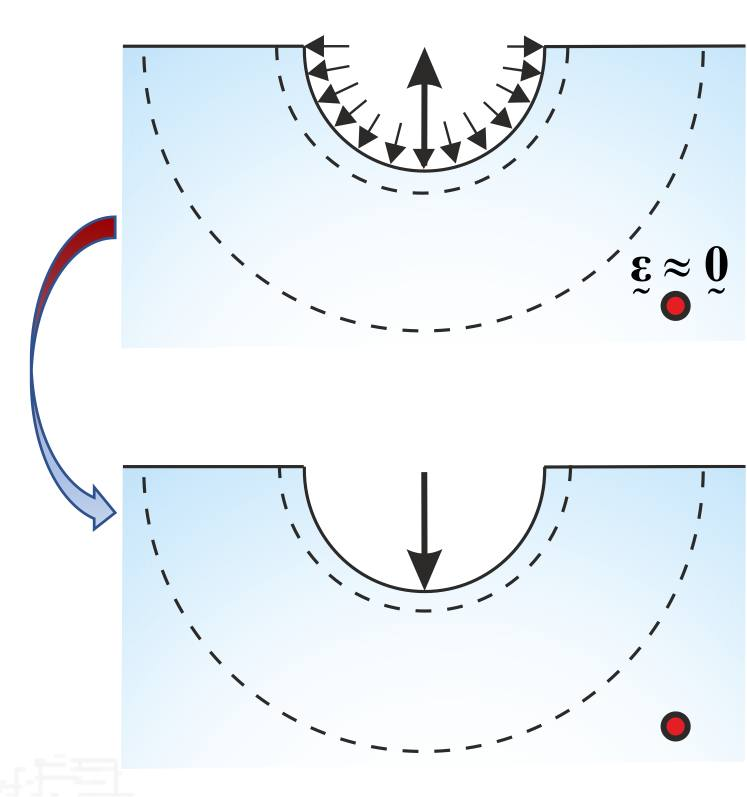
\includegraphics[width=0.4\textwidth]{images/14.1.jpg}
\end{figure}

 

Точный учёт граничных условий (усилий и перемещений) делает краевую
задачу очень сложной. Принцип Сен-Венана гласит, что \textbf{уравновешенная
система внешних сил, приложенная к упругому телу, когда все точки
приложения сил этой системы лежат внутри некоторой сферы, производит
пренебрежимо малые деформации в точках тела, на расстояниях от
сферы, достаточно больших по сравнению с её радиусом.} Таким образом,
при решении задач заданная система сил, приложенная к небольшой части
упругого тела, заменяется другой, удобной для упрощения задачи,
статически эквивалентной системой сил (т.е. имеющей те же главный
вектор и главный момент), приложенной к той же части тела.


\textbf{Простейшие задачи теории упругости} – это краевые задачи равновесия (также называются задачи статики или статические задачи) однородных изотропных тел, в которых в любой точке тела
компоненты напряжений (а значит и деформаций) постоянны или линейно зависят от координат.
Уравнения совместности выполнены тождественно, потому что вторые частные производные от констант
и линейных функций равны нулю. Уравнения Бельтрами-Митчелла выполняются тождественно (что не гарантирует выполнения уравнений равновесия), если
массовые силы являются константами, т. е. не зависят от координат точек тела. В ином случае эти
уравнения являются условиями, которым должны удовлетворять массовые силы, чтобы в теле было
реализовано простейшее напряженно-деформированное состояние.


\textbf{Полуобратный метод Сен-Венана} – метод решения задач, при котором частично задаются напряжения и
перемещения, а затем при помощи уравнений теории упругости определяются условия, которым должны
удовлетворять неизвестные компоненты напряжений и перемещений. На последнем этапе решения
можно воспользоваться формулами Чезаро:
$$
u_i^A=u_i^O+\omega_{j i}^O\left(x_j^A-x_j^O\right)+\int_O^A\left[\varepsilon_{i j}+\left(x_k^A-x_k\right)\left(\varepsilon_{i j, k}-\varepsilon_{j k, i}\right)\right] d x_j.
$$
Упростим формулы Чезаро для случая, когда все компоненты $\varepsilon_{i j, k}$ являются константами: 
Примем за $O$ начало координат и исключим движение абсолютно твердого тела: $x_i^O=u_i^O=\omega_{i j}^O=0$.
Криволинейный интеграл не зависит от пути интегрирования. Предполагая тело выпуклым, соединим точки $O$ и $A$ прямолинейным отрезком и параметризуем переменной $t \in[0 ; 1]$.

\begin{figure}[h!]
  \centering
  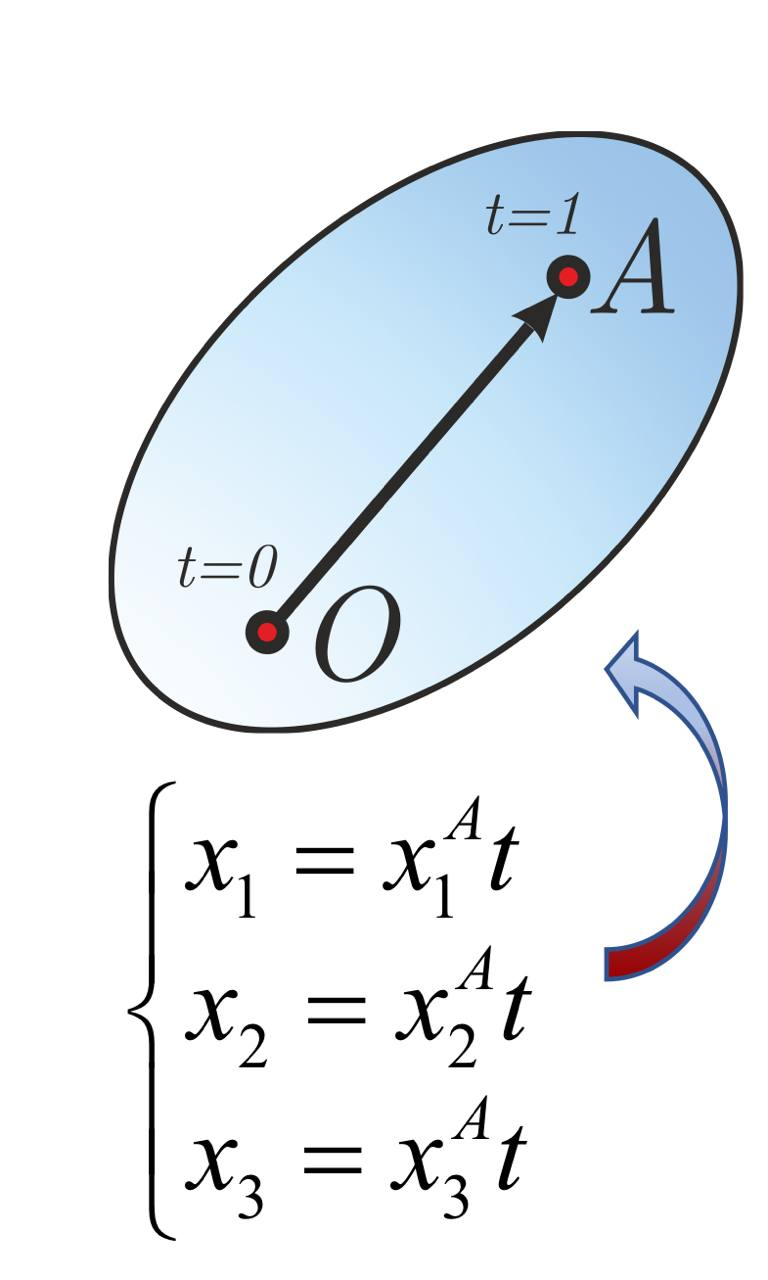
\includegraphics[width=0.2\textwidth]{images/14.2.jpg}  
\end{figure}

Тогда 
$$
\begin{aligned}
& \begin{array}{l}
x_k=x_k^A t \\
x_j=x_j^A t
\end{array}: \int_0^A\left(x_k^A-x_k\right)\left(\varepsilon_{i j, k}-\varepsilon_{j k, i}\right) d x_j=\left(\varepsilon_{i j, k}-\varepsilon_{j k, i}\right) \int_0^1\left(x_k^A-x_k^A t\right) x_j^A d t= \\
& =\left(\varepsilon_{i j, k}-\varepsilon_{j k, i}\right) x_k^A x_j^A \int_0^1(1-t) d t=\frac{\left(\varepsilon_{i j, k}-\varepsilon_{j k, i}\right)}{2} x_k^A x_j^A \\
& u_i=x_j \int_0^1 \varepsilon_{i j}^1\left(x_1 t, x_2 t, x_3 t\right) d t+\frac{x_k x_j}{2}\left(\varepsilon_{i j, k}-\varepsilon_{j k, i}\right)
\end{aligned}
$$

Если все компоненты постоянны:$\displaystyle u_i=x_j \int_0^1 \varepsilon_{i j} d t =  x_j \varepsilon_{i j} \int_0^1 d t=\varepsilon_{i j} x_j$


$\displaystyle
u_i=\varepsilon_{i j} x_j, \vec{u}=\underset{\sim}{\varepsilon} \cdot \vec{r}=\vec{r} \cdot \underset{\sim}{\varepsilon} \Rightarrow
\vec{u}=\vec{u}^O-{\underset{\sim}{\omega}}^O \cdot \vec{r}+\underset{\sim}{\varepsilon} \cdot \vec{r}=\vec{u}^O+\left(\underset{\sim}{\varepsilon}-{\underset{\sim}{\omega}}^O\right) \cdot \vec{r}
$


\textbf{Задача о растяжении призматическиого бруса под действием собственного веса.}

\begin{figure}[h!]
  \centering
  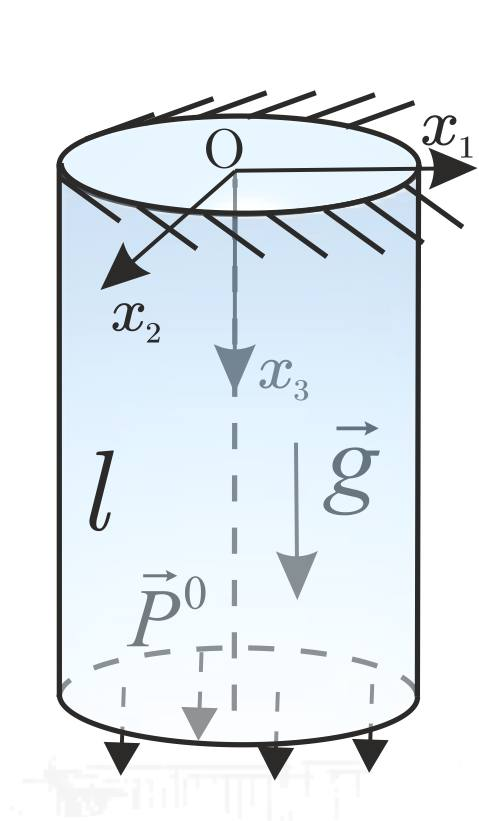
\includegraphics[width=0.15\textwidth]{images/14.3.jpg}    
\end{figure}


Призматический брус закреплен вертикально в поле силы тяжести. Начало координат выбрали в центре масс закрепленного торца. Третья координатная ось вдоль оси бруса. $\vec{F}=g \vec{\kappa}_3$. Предположим, что: $\sigma_{i j}=\left(a x_3+b\right) \delta_{i 3} \delta_{j 3}$. Уравнения Бельтрами-Митчелла выполнены. Также выполнены первых два уравнения равновесия. Подставим в третье: $\sigma_{3 j, j}=-\rho g \Rightarrow a=-\rho g \Rightarrow \sigma_{i j}=\left(-\rho g x_3+b\right) \delta_{i 3} \delta_{j 3}$. Проверим свободу от нагрузки на боковой поверхности бруса, где $\vec{n}=\left(n_1, n_2, 0\right):\left.P_i^{(\vec{n})}\right|_{\Sigma_{\text {bos }}}=\sigma_{i j} n_j=\left(a x_3+b\right) \delta_{i 3} \delta_{j 3} n_j=0$. На нижнем торце бруса имеем $\vec{n}=(0,0,1):\left.P_i^{(\bar{n})}\right|_{\Sigma_{\max }}(a l+b) \delta_{i 3} \delta_{j 3} n_j=(a l+b) \delta_{i 3}=0$.
Получаем: $b=-a l \Rightarrow \sigma_{i j}=\rho g\left(l-x_3\right) \delta_{i 3} \delta_{j 3}$. Определим усилия на верхнем торце $\vec{n}=(0,0,-1)$ : $\left.P_i^{(\bar{n})}\right|_{\Sigma_{\mathrm{segs}}}=-\rho g l \delta_{i 3} \Rightarrow P S=\rho g l S=M g$. Такое распределение соответствует идеальному закреплению, когда существуют только нормальные равномерно распределенные напряжения.
$$
\left[\sigma_{i j}\right]=\rho g\left(l-x_3\right)\left(\begin{array}{lll}
0 & 0 & 0 \\
0 & 0 & 0 \\
0 & 0 & 1
\end{array}\right)
$$
Принцип Сен-Венана позволяет применять найденные формулы вдали от зоны закрепления и при неидеальном закреплении. Далее, применяем обобщенный закон Гука и находим компоненты тензора деформаций Коши:
$ \sigma_{i j}= \rho g\left(l-x_3\right) \delta_{i 3} \delta_{j 3} ;\quad \sigma=\frac{\sigma_{k k}}{3}=\frac{\rho g}{3}\left(l-x_3\right) \Rightarrow \varepsilon_{i j}=-\frac{3 v}{E} \sigma \delta_{i j}+\frac{1+v}{E} \sigma_{i j}=\left(-\frac{v}{E} \delta_{i j}+\frac{1+v}{E} \delta_{i 3} \delta_{j 3}\right) \rho g\left(l-x_3\right) \varepsilon_{11}= \varepsilon_{22}=-\frac{v}{E} \rho g\left(l-x_3\right) ; \varepsilon_{33}=\frac{\rho g}{E}\left(l-x_3\right) ; \varepsilon_{12}=\varepsilon_{13}=\varepsilon_{23}=0.$


Компоненты деформаций зависят только от $x_3$, а матрица - диагональная.
$ \displaystyle
u_1=x_j \int_0^1 \varepsilon_{1 j}\left(x_3 t\right) d t+\frac{x_k x_j}{2}\left(\varepsilon_{1 j, k}-\varepsilon_{j k, 1}\right)=x_1 \int_0^1 \varepsilon_{11}\left(x_3 t\right) d t+\frac{x_3 x_1}{2} \varepsilon_{11,3}=\frac{v x_1}{E x_3} \rho g \int_0^1\left(l-x_3 t\right) d\left(l-x_3 t\right)+\frac{x_3 x_1}{2} \frac{v}{E} \rho g=\left.\frac{v x_1}{E} \frac{\rho g}{2 x_3}\left(l-x_3 t\right)^2\right|_0 ^1+\frac{x_3 x_1}{2} \frac{v}{E} \rho g=\frac{v \rho g}{2 E} x_1\left(\frac{\left(l-x_3\right)^2-l^2}{x_3}+x_3\right)=-\frac{v \rho g}{E} x_1\left(l-x_3\right) u_2= x_j \int_0^1 \varepsilon_{2 j} d t+\frac{x_k x_j}{2}\left(\varepsilon_{2 j, k}-\varepsilon_{j k, 2}\right)=x_2 \int_0^1 \varepsilon_{22}\left(x_3 t\right) d t+\frac{x_3 x_2}{2} \varepsilon_{22,3}=\frac{v x_2}{E x_3} \rho g \int_0^1\left(l-x_3 t\right) d\left(l-x_3 t\right)+\frac{x_3 x_2}{2} \frac{v}{E} \rho g=\left.\frac{v x_2}{E x_3} \rho g \frac{\left(l-x_3 t\right)^2}{2}\right|_0 ^1+\frac{x_3 x_2}{2} \frac{v}{E} \rho g=\frac{v \rho g}{2 E} x_2\left(\frac{\left(l-x_3\right)^2-l^2}{x_3}+x_3\right)=-\frac{v \rho g}{E} x_2\left(l-x_3\right)$

$ \displaystyle
u_3=x_j \int_0^1 \varepsilon_{3 j} d t+\frac{x_k x_j}{2}\left(\varepsilon_{3 j, k}-\varepsilon_{j k, 3}\right)=x_3 \int_0^1 \varepsilon_{33} d t+\frac{x_k x_j}{2} \varepsilon_{3 j, k}-\frac{x_k x_j}{2} \varepsilon_{j k, 3}=x_3 \int_0^1 \varepsilon_{33}\left(x_3 t\right) d t+\frac{x_3 x_3}{2} \varepsilon_{33,3}
-\frac{x_3 x_3}{2} \varepsilon_{33,3}-\frac{x_2 x_2}{2} \varepsilon_{22,3}-\frac{x_1 x_1}{2} \varepsilon_{11,3}=-\frac{\rho g}{E} \int_0^1\left(l-x_3 t\right) d\left(-x_3 t\right)-\frac{v \rho g}{2 E}\left[\left(x_2\right)^2+\left(x_1\right)^2\right]
=-\left.\frac{\rho g}{E} \frac{\left(l-x_3 t\right)^2}{2}\right|_0 ^1-\frac{v \rho g}{2 E}\left[\left(x_2\right)^2+\left(x_1\right)^2\right]=-\frac{\rho g}{2 E}\left(\left(x_3\right)^2+v\left[\left(x_2\right)^2+\left(x_1\right)^2\right]-2 l x_3\right)$


$$ \text{Получаем:}\quad u_1=-\frac{v}{E} \rho g\left(l-x_3\right) x_1 ; \quad u_2=-\frac{v}{E} \rho g\left(l-x_3\right) x_2;  $$
$$ u_3=-\frac{\rho g}{2 E}\left(\left(x_3\right)^2+v\left(\left(x_1\right)^2+\left(x_2\right)^2\right)-2 l x_3\right)$$


\vfill

\section{Ослабление граничных условий: принцип Сен-Венана. Определение простейших задачах теории упругости. Формула Чезаро для простейших задач. Полуобратный метод Сен-Венана: решение задачи о кручении призматического бруса круглого сечения.}

\begin{figure}[h!]
  \centering
  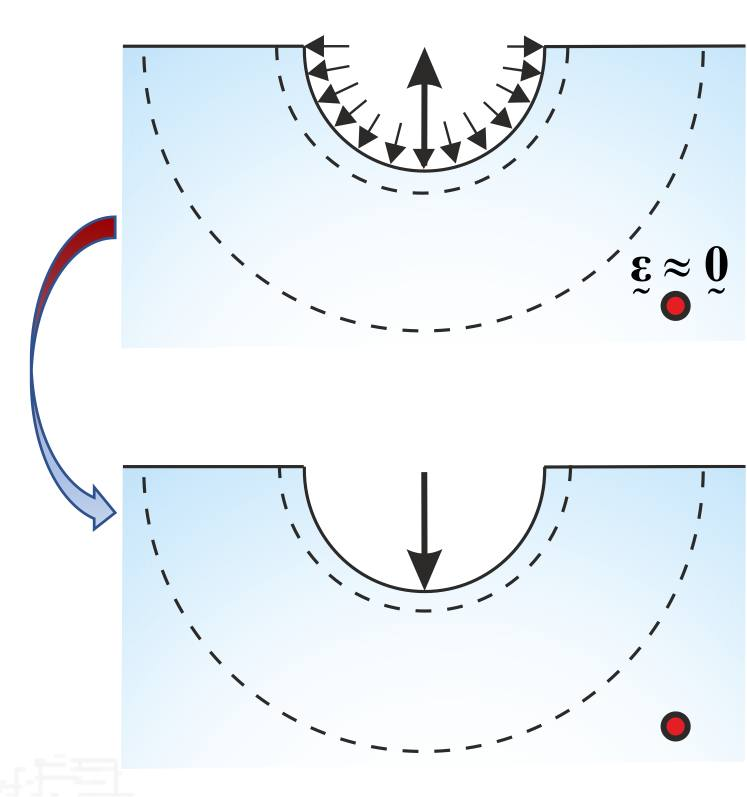
\includegraphics[width=0.4\textwidth]{images/14.1.jpg}   
\end{figure}


Точный учёт граничных условий (усилий и перемещений) делает краевую
задачу очень сложной. Принцип Сен-Венана гласит, что \textbf{уравновешенная
система внешних сил, приложенная к упругому телу, когда все точки
приложения сил этой системы лежат внутри некоторой сферы, производит
пренебрежимо малые деформации в точках тела, на расстояниях от
сферы, достаточно больших по сравнению с её радиусом.} Таким образом,
при решении задач заданная система сил, приложенная к небольшой части
упругого тела, заменяется другой, удобной для упрощения задачи,
статически эквивалентной системой сил (т.е. имеющей те же главный
вектор и главный момент), приложенной к той же части тела.


\textbf{Простейшие задачи теории упругости} – это краевые задачи равновесия (также называются задачи статики или статические задачи) однородных изотропных тел, в которых в любой точке тела
компоненты напряжений (а значит и деформаций) постоянны или линейно зависят от координат.
Уравнения совместности выполнены тождественно, потому что вторые частные производные от констант
и линейных функций равны нулю. Уравнения Бельтрами-Митчелла выполняются тождественно (что не гарантирует выполнения уравнений равновесия), если
массовые силы являются константами, т. е. не зависят от координат точек тела. В ином случае эти
уравнения являются условиями, которым должны удовлетворять массовые силы, чтобы в теле было
реализовано простейшее напряженно-деформированное состояние.


\textbf{Полуобратный метод Сен-Венана} – метод решения задач, при котором частично задаются напряжения и
перемещения, а затем при помощи уравнений теории упругости определяются условия, которым должны
удовлетворять неизвестные компоненты напряжений и перемещений. На последнем этапе решения
можно воспользоваться формулами Чезаро:
$$
u_i^A=u_i^O+\omega_{j i}^O\left(x_j^A-x_j^O\right)+\int_O^A\left[\varepsilon_{i j}+\left(x_k^A-x_k\right)\left(\varepsilon_{i j, k}-\varepsilon_{j k, i}\right)\right] d x_j.
$$
Упростим формулы Чезаро для случая, когда все компоненты $\varepsilon_{i j, k}$ являются константами: 
Примем за $O$ начало координат и исключим движение абсолютно твердого тела: $x_i^O=u_i^O=\omega_{i j}^O=0$.
Криволинейный интеграл не зависит от пути интегрирования. Предполагая тело выпуклым, соединим точки $O$ и $A$ прямолинейным отрезком и параметризуем переменной $t \in[0 ; 1]$.

\begin{figure}[h!]
  \centering
  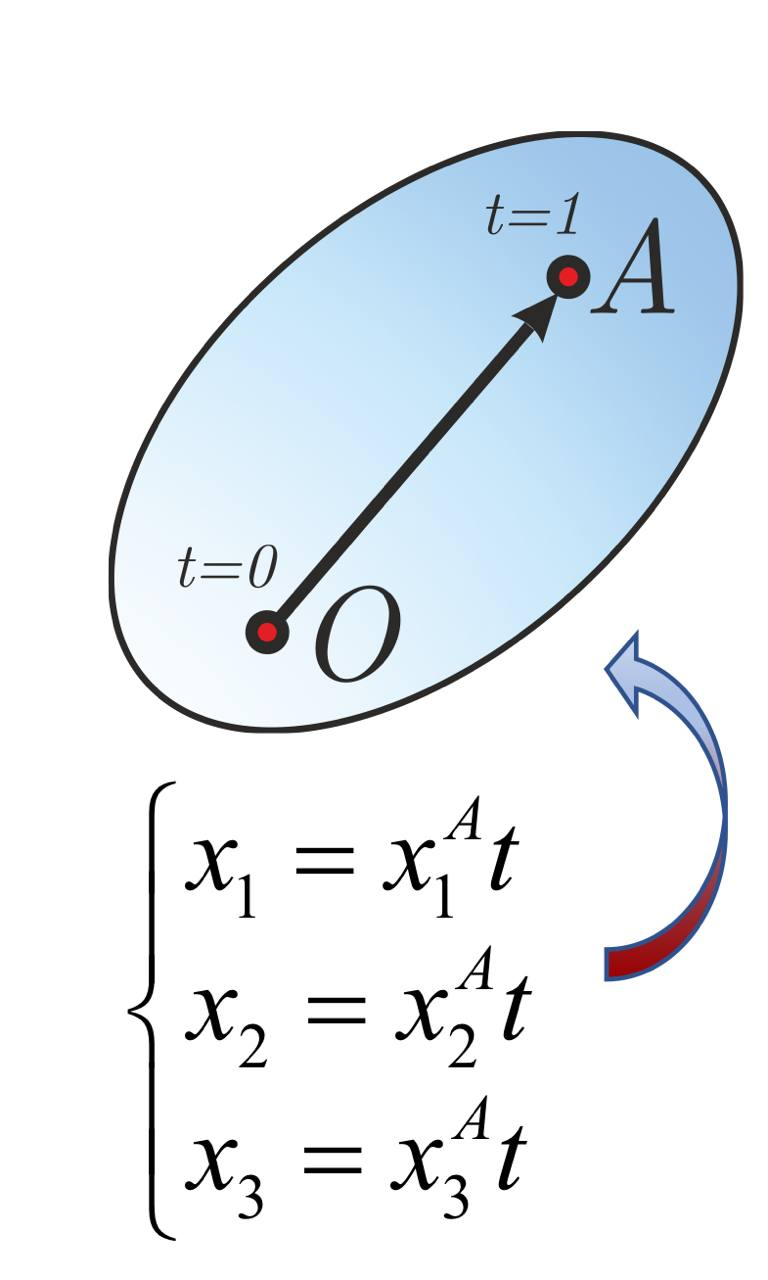
\includegraphics[width=0.2\textwidth]{images/14.2.jpg}   
\end{figure}

Тогда  
$$
\begin{aligned}
& \begin{array}{l}
x_k=x_k^A t \\
x_j=x_j^A t
\end{array}: \int_0^A\left(x_k^A-x_k\right)\left(\varepsilon_{i j, k}-\varepsilon_{j k, i}\right) d x_j=\left(\varepsilon_{i j, k}-\varepsilon_{j k, i}\right) \int_0^1\left(x_k^A-x_k^A t\right) x_j^A d t= \\
& =\left(\varepsilon_{i j, k}-\varepsilon_{j k, i}\right) x_k^A x_j^A \int_0^1(1-t) d t=\frac{\left(\varepsilon_{i j, k}-\varepsilon_{j k, i}\right)}{2} x_k^A x_j^A \\
& u_i=x_j \int_0^1 \varepsilon_{i j}^1\left(x_1 t, x_2 t, x_3 t\right) d t+\frac{x_k x_j}{2}\left(\varepsilon_{i j, k}-\varepsilon_{j k, i}\right)
\end{aligned}
$$
Если все компоненты постоянны:$\displaystyle u_i=x_j \int_0^1 \varepsilon_{i j} d t =  x_j \varepsilon_{i j} \int_0^1 d t=\varepsilon_{i j} x_j$


$\displaystyle
u_i=\varepsilon_{i j} x_j, \vec{u}=\underset{\sim}{\varepsilon} \cdot \vec{r}=\vec{r} \cdot \underset{\sim}{\varepsilon} \Rightarrow
\vec{u}=\vec{u}^O-{\underset{\sim}{\omega}}^O \cdot \vec{r}+\underset{\sim}{\varepsilon} \cdot \vec{r}=\vec{u}^O+\left(\underset{\sim}{\varepsilon}-{\underset{\sim}{\omega}}^O\right) \cdot \vec{r}
$


\textbf{Задача о кручении призматического бруса круглого сечения}


На торцах круглого призматического бруса с осью $Ox_3$  действуют пары сил,
моменты которых равны по величине и имеют противоположные знаки.

\begin{figure}[h!]
  \centering
  \subfigure{
    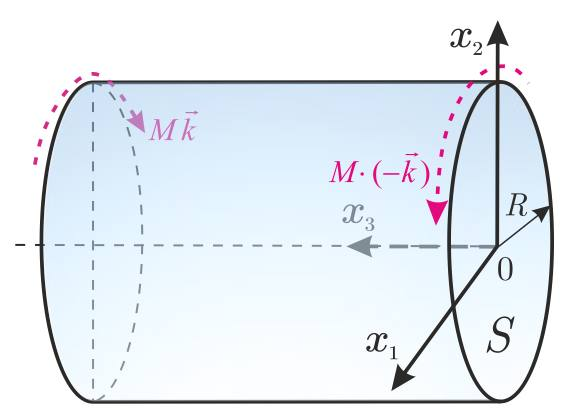
\includegraphics[width=0.5\textwidth]{images/16.1.jpg}}
  \subfigure{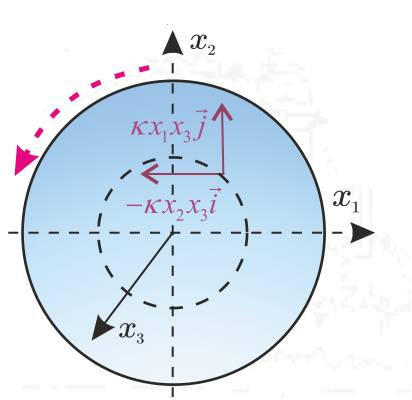
\includegraphics[width=0.4\textwidth]{images/16.2.jpg}}  
\end{figure}


Боковая
поверхность свободна, массовые силы не учитываются. Предположим, что
возникшая деформация чистого кручения описывается тензором деформации:
$$
\left[\varepsilon_{i j}\right]=\left(\begin{array}{ccc}
0 & 0 & -\frac{\kappa}{2} x_2 \\
0 & 0 & \frac{\kappa}{2} x_1 \\
-\frac{\kappa}{2} x_2 & \frac{\kappa}{2} x_1 & 0
\end{array}\right)
$$
Исключим движение абсолютно твердого тела
и найдем вектор перемещения из формул Чезаро, приняв: $u_i^O=\omega_{ji}^O=x_i^O=0$
Учтем, что диагональные элементы равны нулю и нет зависимости от $x_3$:


$ \displaystyle
u_1=x_j \int_0^1 \varepsilon_{1 j} d t+\frac{x_k x_j}{2}\left(\varepsilon_{1 j, k}-\varepsilon_{j k, 1}\right)=x_3 \int_0^1 \varepsilon_{13} d t+\frac{x_2 x_3}{2} \varepsilon_{13,2}-\frac{x_3 x_2}{2} \varepsilon_{23,1}-\frac{x_2 x_3}{2} \varepsilon_{32,1}
=x_3 \int_0^1\left(-\frac{\kappa x_2 t}{2}\right) d t+\frac{x_2 x_3}{2} \varepsilon_{13,2}-x_2 x_3 \varepsilon_{23,1}=\frac{-\kappa}{2} x_2 x_3 \int_0^1 t d t-\frac{\kappa}{2} \frac{x_2 x_3}{2}-\frac{\kappa}{2} x_2 x_3=\left(-\frac{1}{2} \frac{1}{2}-\frac{1}{4}-\frac{1}{2}\right) \kappa x_2 x_3=-\kappa x_2 x_3$


$ \displaystyle
u_2=x_j \int_0^1 \varepsilon_{2 j} d t+\frac{x_k x_j}{2}\left(\varepsilon_{2 j, k}-\varepsilon_{j k, 2}\right)=x_3 \int_0^1 \varepsilon_{23} d t+\frac{x_1 x_3}{2} \varepsilon_{23,1}-\frac{x_3 x_1}{2} \varepsilon_{13,2}-\frac{x_1 x_3}{2} \varepsilon_{31,2}=x_3 \int_0^1 \frac{\kappa x_1 t}{2} d t
+\frac{x_1 x_3}{2} \varepsilon_{23,2}-x_1 x_3 \varepsilon_{13,2}=\frac{\kappa}{2} x_1 x_3 \int_0^1 t d t+\frac{\kappa}{2} \frac{x_1 x_3}{2}+\frac{\kappa}{2} x_1 x_3=\frac{\kappa}{2} x_1 x_3 \frac{1}{2}+\frac{\kappa x_1 x_3}{4}+\frac{\kappa}{2} x_1 x_3=\kappa x_1 x_3$


$\displaystyle
u_3= x_j \int_0^1 \varepsilon_{3 j} d t+\frac{x_k x_j}{2}\left(\varepsilon_{3 j, k}-\varepsilon_{j k, 3}\right)=x_1 \int_0^1 \varepsilon_{31} d t+x_2 \int_0^1 \varepsilon_{32} d t+\frac{x_2 x_1}{2} \varepsilon_{31,2}+\frac{x_1 x_2}{2} \varepsilon_{32,1}=x_1 \int_0^1-\frac{\kappa x_2 t}{2} d t+x_2 \int_0^1 \frac{\kappa x_1 t}{2} d t+\frac{x_2 x_1}{2}(-\kappa)+\frac{x_1 x_2}{2} \kappa=0 $


Получаем: $\quad u_1=-\kappa x_2 x_3 ; \quad u_2=\kappa x_1 x_3; \quad u_3=0 \quad \Rightarrow \quad$ Поперечные сечения остаются
плоскими и поворачиваются на
некоторый угол, который
различен для разных сечений.


Закон Гука при кручении круглого призматического бруса:
$$
-G \kappa I_O \vec{k}={\vec{L}=M \cdot(-\vec{k})} \Rightarrow \kappa=\frac{M}{G I_O}
$$


\section{Ослабление граничных условий: принцип Сен-Венана. Определение простейших задачах теории упругости. Формула Чезаро для простейших задач. Полуобратный метод Сен-Венана: решение задачи о чистом изгибе призматического бруса.}

\begin{figure}[h!]
  \centering
  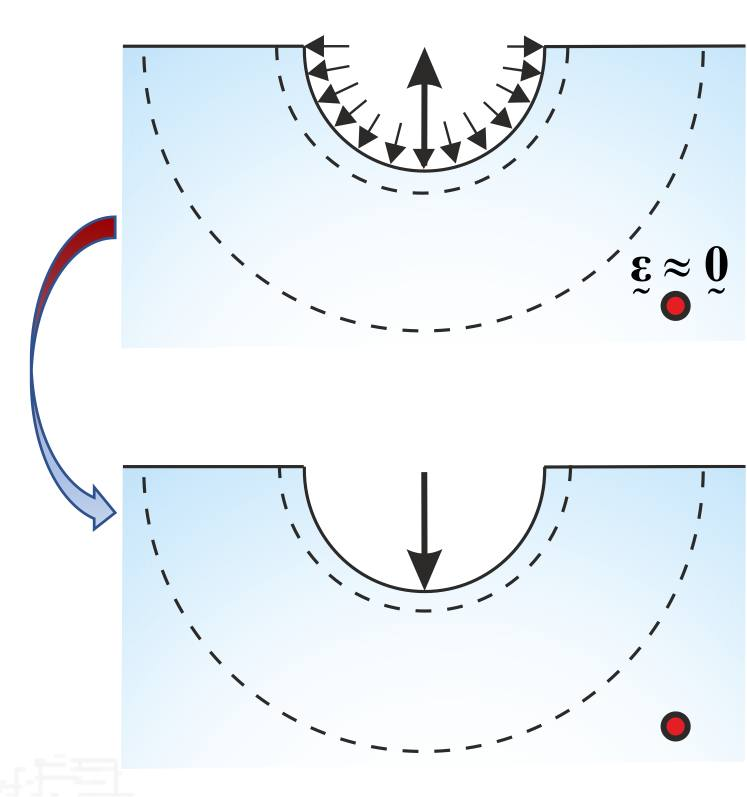
\includegraphics[width=0.4\textwidth]{images/14.1.jpg} 
\end{figure}


Точный учёт граничных условий (усилий и перемещений) делает краевую
задачу очень сложной. Принцип Сен-Венана гласит, что \textbf{уравновешенная
система внешних сил, приложенная к упругому телу, когда все точки
приложения сил этой системы лежат внутри некоторой сферы, производит
пренебрежимо малые деформации в точках тела, на расстояниях от
сферы, достаточно больших по сравнению с её радиусом.} Таким образом,
при решении задач заданная система сил, приложенная к небольшой части
упругого тела, заменяется другой, удобной для упрощения задачи,
статически эквивалентной системой сил (т.е. имеющей те же главный
вектор и главный момент), приложенной к той же части тела.


\textbf{Простейшие задачи теории упругости} – это краевые задачи равновесия (также называются задачи статики или статические задачи) однородных изотропных тел, в которых в любой точке тела
компоненты напряжений (а значит и деформаций) постоянны или линейно зависят от координат.
Уравнения совместности выполнены тождественно, потому что вторые частные производные от констант
и линейных функций равны нулю. Уравнения Бельтрами-Митчелла выполняются тождественно (что не гарантирует выполнения уравнений равновесия), если
массовые силы являются константами, т. е. не зависят от координат точек тела. В ином случае эти
уравнения являются условиями, которым должны удовлетворять массовые силы, чтобы в теле было
реализовано простейшее напряженно-деформированное состояние.


\textbf{Полуобратный метод Сен-Венана} – метод решения задач, при котором частично задаются напряжения и
перемещения, а затем при помощи уравнений теории упругости определяются условия, которым должны
удовлетворять неизвестные компоненты напряжений и перемещений. На последнем этапе решения
можно воспользоваться формулами Чезаро:
$$
u_i^A=u_i^O+\omega_{j i}^O\left(x_j^A-x_j^O\right)+\int_O^A\left[\varepsilon_{i j}+\left(x_k^A-x_k\right)\left(\varepsilon_{i j, k}-\varepsilon_{j k, i}\right)\right] d x_j.
$$
Упростим формулы Чезаро для случая, когда все компоненты $\varepsilon_{i j, k}$ являются константами: 
Примем за $O$ начало координат и исключим движение абсолютно твердого тела: $x_i^O=u_i^O=\omega_{i j}^O=0$.
Криволинейный интеграл не зависит от пути интегрирования. Предполагая тело выпуклым, соединим точки $O$ и $A$ прямолинейным отрезком и параметризуем переменной $t \in[0 ; 1]$.

\begin{figure}[h!]
  \centering
  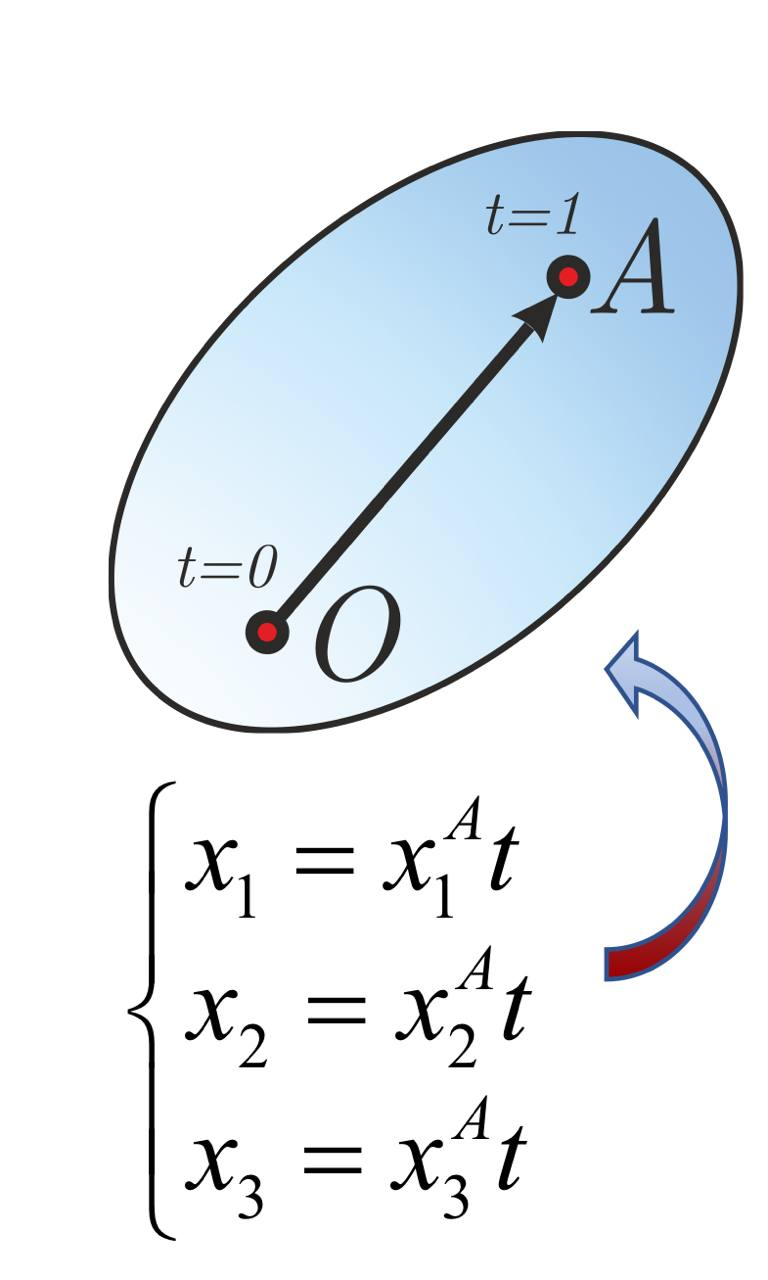
\includegraphics[width=0.2\textwidth]{images/14.2.jpg}
\end{figure}

Тогда   
$$
\begin{aligned}
& \begin{array}{l}
x_k=x_k^A t \\
x_j=x_j^A t
\end{array}: \int_0^A\left(x_k^A-x_k\right)\left(\varepsilon_{i j, k}-\varepsilon_{j k, i}\right) d x_j=\left(\varepsilon_{i j, k}-\varepsilon_{j k, i}\right) \int_0^1\left(x_k^A-x_k^A t\right) x_j^A d t= \\
& =\left(\varepsilon_{i j, k}-\varepsilon_{j k, i}\right) x_k^A x_j^A \int_0^1(1-t) d t=\frac{\left(\varepsilon_{i j, k}-\varepsilon_{j k, i}\right)}{2} x_k^A x_j^A \\
& u_i=x_j \int_0^1 \varepsilon_{i j}^1\left(x_1 t, x_2 t, x_3 t\right) d t+\frac{x_k x_j}{2}\left(\varepsilon_{i j, k}-\varepsilon_{j k, i}\right)
\end{aligned}
$$
Если все компоненты постоянны:$\displaystyle u_i=x_j \int_0^1 \varepsilon_{i j} d t =  x_j \varepsilon_{i j} \int_0^1 d t=\varepsilon_{i j} x_j$


$\displaystyle
u_i=\varepsilon_{i j} x_j, \vec{u}=\underset{\sim}{\varepsilon} \cdot \vec{r}=\vec{r} \cdot \underset{\sim}{\varepsilon} \Rightarrow
\vec{u}=\vec{u}^O-{\underset{\sim}{\omega}}^O \cdot \vec{r}+\underset{\sim}{\varepsilon} \cdot \vec{r}=\vec{u}^O+\left(\underset{\sim}{\varepsilon}-{\underset{\sim}{\omega}}^O\right) \cdot \vec{r}
$



\textbf{Задача о чистом изгибе призматического бруса}

\begin{figure}[h!]
  \centering
  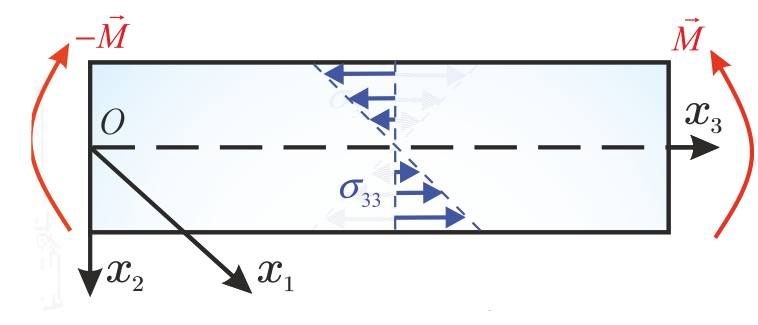
\includegraphics[width=0.5\textwidth]{images/17.1.jpg}  
\end{figure}



Массовыми силами пренебрегаем $\vec{F}=\vec{0}$.
Примем $\sigma_{ij}=ax_2\delta_{i3}\delta_{j3}$.  Уравнения Бельтрами-Митчелла удовлетворяются тождественно. Уравнения
равновесия тоже выполнены: $\sigma_{ij,j}=ax_{2,j}\delta_{i3}\delta_{j3}=a\sigma_{2j}\delta_{i3}\delta_{j3}=a\delta_{i3}\delta_{23}=0$.


Найдем вектор напряжений на боковине с $\vec{n}=(n_1, n_2, 0): P_i^{(\vec{n})}=\sigma_{ij}n_j=0$ 


На торцах с $\vec{n}=(0, 0, \mp1): P_i^{(\mp\vec{k})}=\mp a x_2 \sigma_{i3}$ 


Боковая поверхность является свободной от внешних сил. На торцах
действуют линейно-распределенные нормальные напряжения. Определим главный вектор и главный
момент сил, действующих на торцах:
$$
\int_S P_3^{(\mp \vec{k})} d \Sigma=\mp a \int_S x_2 d \Sigma=\mp a S x_2^{\text{ЦМ}}=0=\int_S P_1^{(\mp \vec{k})} d \Sigma=\int_S P_2^{(\mp \vec{k})} d \Sigma
$$

$I=I_{22}$ - момент инерции
сечения относительно
нейтральной оси $Ox_1$.
(Т.к. $Ox_1$ и $Ox_2$ - главные оси
инерции сечения, то $I_{12}$ = 0.)

$$
\begin{aligned}
& \vec{L}=\int_S \vec{r} \times \vec{P}^{(\vec{k})} d \Sigma=\int_S\left|\begin{array}{ccc}
\vec{i} & \vec{j} & \vec{k} \\
x_1 & x_2 & 0 \\
0 & 0 & a x_2
\end{array}\right| d \Sigma=\left(a \int_S x_2^2 d \Sigma\right) \vec{i}-\left(a \int_S x_1 x_2 d \Sigma\right) \vec{j}= \\
& =a I_{22} \vec{i}-a I_{12} \vec{j}=a I_{22} \vec{i} \equiv a I \cdot \vec{i} 
\end{aligned}
$$
Практически приложить внешние силы вида $\vec{P}^{( \pm \vec{k})}= \pm a x_2 \vec{k}$ невозможно. Следуя принципу Сен-Венана, приложим нагрузку с главным изгибающим моментом: $\vec{M}=\vec{L} \Rightarrow M=a I \Rightarrow \sigma_{i j}=(M / I) x_2 \delta_{i 3} \delta_{j 3}$. По обобщенному закону Гука:
$$
\sigma=\sigma_{k k}=\frac{M}{3 I_{22}} x_2 ; \quad \varepsilon_{i j}=-\frac{3 v}{E} \sigma \delta_{i j}+\frac{1+v}{E} \sigma_{i j}=\left(-\frac{v}{E} \delta_{i j}+\frac{1+v}{E} \delta_{i 3} \delta_{j 3}\right) \frac{M}{I} x_2
$$
$
\displaystyle
 \text { Главные оси бруса совпадают с главными осями тензоров } \\ \text { напряжений и деформаций. Компоненты тензоров зависят } \\ \text { только от } x_2, \text { а матрица в главных осях является диагональной. } \\ \varepsilon_{12}=\varepsilon_{13}=\varepsilon_{23}=0
\varepsilon_{11}=\varepsilon_{22}=-\frac{v M}{E I} x_2 ; \varepsilon_{33}=\frac{M}{E I} x_2 ; \\ u_3=x_j \int_0^1 \varepsilon_{3 j} d t+\frac{x_k x_j}{2}\left(\varepsilon_{3 j, k}-\varepsilon_{j k, 3}\right)=x_3 \int_0^1 \varepsilon_{33}\left(x_2 t\right) d t+\frac{x_2 x_3}{2} \varepsilon_{33,2}=x_3 \frac{M}{E I} x_2 \int_0^1 t d t+\frac{x_2 x_3}{2} \frac{M}{E I}=\frac{M}{E I} x_2 x_3 \\ u_1=x_j \int_0^1 \varepsilon_{1 j} d t+\frac{x_k x_j}{2}\left(\varepsilon_{1 j, k}-\varepsilon_{j k, 1}\right)=x_1 \int_0^1 \varepsilon_{11}\left(x_2 t\right) d t+\frac{x_2 x_1}{2} \varepsilon_{11,2}=\frac{-v M}{E I} x_1 x_2\left(\int_0^1 t d t+\frac{1}{2}\right)=-\frac{v M}{E I} x_1 x_2 \\ u_2=x_j \int_0^1 \varepsilon_{2 j} d t+\frac{x_k x_j}{2}\left(\varepsilon_{2 j, k}-\varepsilon_{j k, 2}\right)=x_2 \int_0^1 \varepsilon_{22} d t+\frac{x_2 x_2}{2} \varepsilon_{22,2}-\frac{x_1 x_1}{2} \varepsilon_{11,2}-\frac{x_2 x_2}{2} \varepsilon_{22,2}-\frac{x_3 x_3}{2} \varepsilon_{33,2} =-\frac{v M}{E I} x_2^2 \int_0^1 t d t+\frac{x_1^2}{2} \frac{v M}{E I}-\frac{x_3^2}{2} \frac{M}{E I}=\frac{-M}{2 E I}\left(x_3^2+v\left[x_2^2-x_1^2\right]\right)$

$$\text{Получаем:} u_2=\frac{-M}{2 E I}\left(x_3^2+v\left[x_2^2-x_1^2\right]\right) ; \quad u_1=-\frac{v M}{E I} x_1 x_2 ; \quad u_3=\frac{M}{E I} x_3 x_2 $$

Найдем, как деформируется ось бруса:
$ x_1=x_2=0 \Rightarrow u_2=\frac{-M}{2 E I} x_3^2, u_1=u_3=0 \Rightarrow$ Ось бруса остается в плоскости изгиба $Ox_2x_3$ и
деформируется в параболу. Кривизна оси бруса с точностью до  малых высшего порядка равна: $ K=\frac{1}{R}=\frac{d^2 u_2}{d x_3{ }^2} \Rightarrow K=\frac{-M}{E I} \Rightarrow $ Закон Гука причистом изгибе: $\frac{1}{R}=\frac{-M}{E I}$



\section{Использование криволинейных координат: задача Ламе о деформировании толстостенной упругой однородной изотропной трубы под действием внешнего и внутреннего давления (кинематическая гипотеза; сведение задачи к краевой задаче обыкновенного дифференциального уравнения; уравнение Леви; формулы ненулевых компонент тензора напряжений).}
Задача Ламе о толстостенной трубе - задача о равновесии цилиндрической трубы, находящейся под действием внутреннего и внешнего давления. $\vec{F}=\overrightarrow{0}$


Кинематическая гипотеза: $\overrightarrow{\mathrm{u}}=u(\rho) \vec{e}_\rho$. 

\begin{figure}[h!]
  \centering
  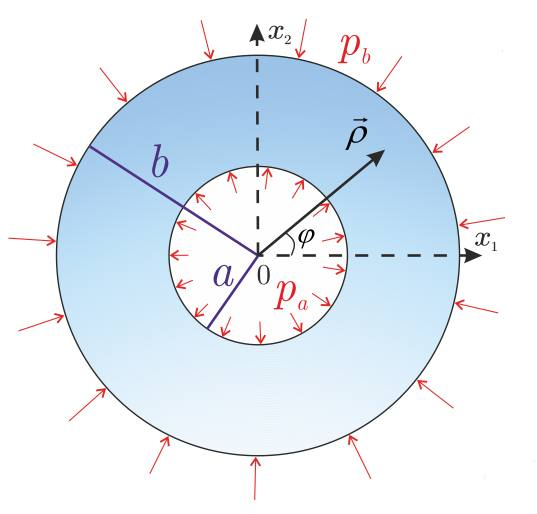
\includegraphics[width=0.4\textwidth]{images/18.1.jpg}
\end{figure}



Запишем
уравнения Ламе и граничные условия в цилиндрической системе координат. 
$ \xi^1=\rho$, $ \xi^2=\varphi$, $\xi^3=z$; $\quad x_1 \equiv x=\rho \cos \varphi$, $x_2 \equiv y=\rho \sin \varphi$, $x_3 \equiv z=z$.
$(\Gamma_{12}^2=\Gamma_{21}^2=1 / \rho, \Gamma_{22}^1=-\rho) $ $(g_{11}=g_{33}=1, g_{22}=\rho^2 ; \sqrt{g}=\rho ; g^{11}=g^{33}=1, g^{22}=\rho^{-2})$
Проверяем кинематическую гипотезу:
$\left\{ \begin{array}{c}
     \vec{e}_\rho=\vec{e}_1=\vec{e^1}\\
     \vec{e}_\varphi=\rho^{-1} \vec{e}_2=\rho \vec{e^2}\\
      \vec{e}_z=\vec{e}_3=\vec{e^{3}}\\
        \end{array}\right.$
$\left\{ \begin{array}{c}
     u_{\rho}=u_1=u^1=u(\rho) \\
      u_{\varphi}=\rho u^2=\rho^{-1} u_2=0\\
      u_z=u^3=u_3=0\\
        \end{array}\right.$
 
$ 
\displaystyle
\mathrm{div} \vec{u}=\frac{\partial u_\rho}{\partial \rho}+\frac{1}{\rho} \frac{\partial u_{\varphi}}{\partial \phi}+\frac{\partial u_z}{\partial z}+\frac{u_\rho}{\rho}=\frac{d u}{d \rho}+\frac{u}{\rho} \Rightarrow \mathrm{grad} \mathrm{div} \vec{u}=\vec{e^i} \frac{\partial \mathrm{div} \vec{u}}{\partial \xi^i}=\vec{e}_\rho \frac{d}{d \rho}\left(\frac{d u}{d \rho}+\frac{u}{\rho}\right)
$

$$
u_{1,2}=\frac{\partial u}{\partial \varphi}-u_q \Gamma_{12}^q=-u_2 \Gamma_{12}^2 \equiv 0 \quad
u_{1,3}=\frac{\partial u}{\partial z}-u_q \Gamma_{13}^q \equiv 0
$$

$$
\mathrm{rot} \vec{u}=\frac{1}{\sqrt{g}} \mathrm{det}\left(\begin{array}{ccc}
\vec{e^1} & \vec{e^2} & \vec{e^3} \\
\nabla_1 & \nabla_2 & \nabla_3 \\
u_1 & 0 & 0
\end{array}\right)=\frac{1}{\sqrt{g}}\left(u_{1,3} \vec{e^2}-u_{1,2} \vec{e^3}\right) \equiv \overrightarrow{0}
$$

Уравнение Ламе в отсутствии массовых сил: $(\lambda+2 \mu) \mathrm{grad} \mathrm{div} \vec{u}+\mu \mathrm{rot} \mathrm{rot} \vec{u}=0$. 

$
\displaystyle
\begin{array}{l}

\mathrm{rot} \vec{u}=0 \stackrel{\vec{F}=\overline{0}}{\Rightarrow} \mathrm{grad} \mathrm{div} \vec{u}=0 \stackrel{\bar{u}={\bar{u_\rho}}(\rho)}{\Rightarrow} \frac{d}{d \rho}\left(\frac{d u}{d \rho}+\frac{u}{\rho}\right)=0 \Leftrightarrow \frac{d}{d \rho}\left(\frac{1}{\rho} \frac{d(\rho u)}{d \rho}\right)=0 \Leftrightarrow \frac{d(\rho u)}{d \rho}= \\ =A \rho \Leftrightarrow 
u=\frac{A \rho}{2}+\frac{B}{\rho} \quad u^{\prime}=\frac{A}{2}-\frac{B}{\rho^2}
\end{array}
$


$
\varepsilon_{i j} =\frac{1}{2}\left(u_{j, i}+u_{i, j}\right)=\frac{1}{2}(\frac{\partial u_j}{\partial \xi^i}-u_q \Gamma_{j i}^q+\frac{\partial u_i}{\partial \xi^j}-u_q \Gamma_{i j}^q)=\frac{1}{2}\left(\frac{\partial u_i}{\partial \xi^j}+\frac{\partial u_j}{\partial \xi^i}\right)-u_q \Gamma_{i j}^q= \frac{1}{2}\left(\frac{\partial u_1}{\partial \xi^1}+\frac{\partial u_1}{\partial \xi^1}\right) \delta_{i 1} \delta_{j 1}-u_1 \Gamma_{22}^1 \delta_{i 2} \delta_{j 2}=u^{\prime} \delta_{i 1} \delta_{j 1}+\rho u \delta_{i 2} \delta_{j 2}=\left(\frac{A \rho}{2}-\frac{B}{\rho^2}\right) \delta_{i 1} \delta_{j 1}+\left(\frac{A}{2} \rho^2+B\right) \delta_{i 2} \delta_{j 2}
$

$\left\{ \begin{array}{c}
    \varepsilon^{i j}=g^{i p} g^{j q} \varepsilon_{p q}\\
    \varepsilon_i^j=g^{j q} \varepsilon_{i q} \\
        \end{array}\right.
$ 

$\left\{ \begin{array}{c}
    \varepsilon_{11}=u^{\prime} =\frac{A}{2}-\frac{B}{\rho^2} \\
    \varepsilon_{22}=\rho u  \\
     \varepsilon_{12}=\varepsilon_{13}=\varepsilon_{23}=\varepsilon_{33}=0 \\
        \end{array}\right.
$

$\left\{\begin{array}{c}
   \varepsilon_1^1=\varepsilon^{11}=\varepsilon_{\rho \rho}=u^{\prime} \\
   \varepsilon^{22}=\rho^{-3} u \\
     \varepsilon_2^2=\rho^{-1} u=\varepsilon_{\varphi \varphi}\\
      \varepsilon_{z z}=\varepsilon_3^3=\varepsilon^{12}=\varepsilon^{13}=\varepsilon_{i=j}^{23}=\varepsilon^{33}=\varepsilon_2^1=\varepsilon_3^1=\varepsilon_3^2=\varepsilon_3^3=0 \\
        \end{array}\right.$


$\theta=\varepsilon_i^i=u^{\prime}+\rho^{-1} u=A \Rightarrow \theta=A $
(одинакова во всех точках)

Закон Гука:
$
\sigma_i^j=\lambda \theta \delta_i^j+2 \mu \varepsilon_i^j \Rightarrow \sigma_{i i}^{\phi \text { физ }}=A \lambda+2 \mu \varepsilon_{i i}^{\phi \text { физ }} \quad(j=i) \text {. } 
$
$\left\{ \begin{array}{c}
    \sigma_{\rho \rho}=A \lambda+2 \mu u^{\prime}\\
     \sigma_{\varphi \varphi}=A \lambda+2 \mu \rho^{-1} u  \\
   \sigma_{z z}=A \lambda \\
    \sigma_{\rho \varphi}=\sigma_{\rho z}=\sigma_{\varphi z}=0 \\
        \end{array}\right.
$ 


$
\sigma_{\rho \rho}+\sigma_{\varphi \varphi}=2 A \lambda+2 \mu\left(u^{\prime}+\rho^{-1} u\right)=2 A(\lambda+\mu)=\sigma_{z z} \cdot 2(\lambda+\mu) / \lambda=\sigma_{z z} / v
$


\textbf{Уравнение Леви:} $\quad \sigma_{z z}=v\left(\sigma_{\rho \rho}+\sigma_{\varphi \varphi}\right)$



$
\begin{aligned}
\vec{n} &= -\vec{e}_\rho \quad \Rightarrow \quad \vec{P}^{(-\vec{e}_\rho)}\Big|_{\rho=a} = \sigma^{ij} n_i \vec{e}_j = -\sigma^{1j} \vec{e}_j = -\sigma_{\rho\rho} \vec{e}_\rho \\
\vec{n} &= \vec{e}_\rho \quad \Rightarrow \quad \vec{P}^{(\vec{e}_\rho)}\Big|_{\rho=b} = \sigma^{ij} n_i \vec{e}_j = \sigma^{1j} \vec{e}_j = \sigma_{\rho\rho} \vec{e}_\rho
\end{aligned}$

\begin{figure}[h!]
  \centering
  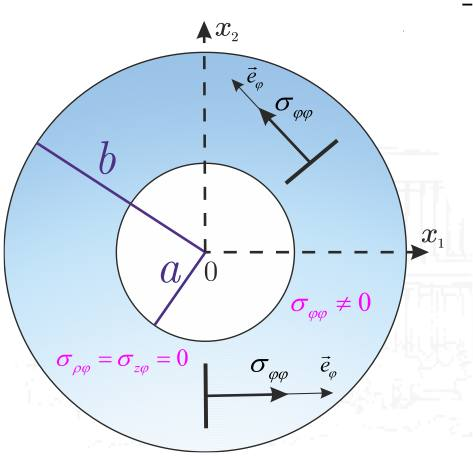
\includegraphics[width=0.4\textwidth]{images/18.2.jpg}
\end{figure}


$\begin{aligned}
& \begin{array}{l}-\left.\sigma_{\rho \rho}\right|_{\rho=a}=p_a \Rightarrow A \lambda+\mu\left(A-2 a^{-2} B\right)=-p_a \\ \left.\sigma_{\rho \rho}\right|_{\rho=b}=-p_b \Rightarrow A \lambda+\mu\left(A-2 b^{-2} B\right)=-p_b\end{array} \quad \Rightarrow\left\{\begin{array}{l}2 \mu a^{-2} B-(\lambda+\mu) A=p_a \\ 2 \mu b^{-2} B-(\lambda+\mu) A=p_b\end{array}\right. \\ & A=\frac{p_a b^{-2}-p_b a^{-2}}{(\lambda+\mu)\left(a^{-2}-b^{-2}\right)} ; \quad B=\frac{p_a-p_b}{2 \mu\left(a^{-2}-b^{-2}\right)} \Rightarrow \\ & A=\frac{p_a a^2-p_b b^2}{(\lambda+\mu)\left(b^2-a^2\right)} ; \quad B=\frac{a^2 b^2\left(p_a-p_b\right)}{2 \mu\left(b^2-a^2\right)} \\ & \sigma_{\rho \rho} (\rho) =\frac{p_a a^2-p_b b^2}{b^2-a^2}-\frac{a^2 b^2\left(p_a-p_b\right)}{b^2-a^2} \frac{1}{\rho^2}=\frac{p_a a^2}{b^2-a^2}\left(1-\frac{b^2}{\rho^2}\right)-\frac{p_b b^2}{b^2-a^2}\left(1-\frac{a^2}{\rho^2}\right) \\ & \sigma_{\varphi\varphi}(\rho)=A \lambda+2 \mu \rho^{-1} u=A \lambda+\mu\left(A+2 \rho^{-2} B\right)=A(\lambda+\mu)+2 \mu B \rho^{-2}\
\\ &\sigma_{\varphi \varphi}(\rho)=\frac{p_a a^2}{b^2-a^2}\left(1+\frac{b^2}{\rho^2}\right)-\frac{p_b b^2}{b^2-a^2}\left(1+\frac{a^2}{\rho^2}\right)\ &
\\ & \end{aligned}$

При условии: $b>a, a \approx b, p_a \gg p_b \Rightarrow A>0, B>0$ 
$$
\sigma_{\varphi \varphi}>0, \max \left|\sigma_{\varphi \varphi}\right|=\sigma_{\varphi \varphi}(a)=\frac{p_a a^2+b^2\left(p_a-2 p_b\right)}{b^2-a^2}
$$
$$
\sigma_{z z}=v\left(\sigma_{\rho \rho}+\sigma_{\varphi \varphi}\right)=2 v \frac{p_a a^2-p_b b^2}{b^2-a^2}>0
$$
Компоненты завяисят только от геометрических характеристик трубы.

\section{Эффективные определяющие соотношения. Эффективный модуль Фойхта. Прямая формула смесей.}
- \textbf{Определяющие соотношения} - это соотношения между причинами и следствиями процессов, которые происходят в телах. Примеры: уравнение Менделеева-Клайперона; закон Гука; закон Навье-Стокса.

- \textbf{Эффективные определяющие соотношения} - это соотношения, связывающие между собой средние по представительному объёму значения причин и следствий. Материальные константы и материальные функции, входящие в эти соотношения, называются эффективными физико-механическими свойствами (характеристиками) композита.

- Экспериментальное определение всего комплекса эффективных свойств композита является дорогим и долгим процессом. Поэтому необходимы математические методы вычисления эффективных характеристик, позволяющие с разной степенью точности вычислять эффективные свойства.

- В МДТТ под эффективными определяющими соотношениями понимаются соотношения позволяющие выразить средние напряжения через средние деформации ( $\langle\underset{\sim}{\boldsymbol{\sigma}}\rangle \sim\langle\underset{\sim}{\boldsymbol{\varepsilon}}\rangle$ - это прямые соотношения), либо наоборот средние деформации через средние напряжения ($\langle\underset{\sim}{\boldsymbol{\varepsilon}}\rangle \sim\langle\underset{\sim}{\boldsymbol{\sigma}}\rangle$ - это обратные соотношения).

- Материальные константы и материальные функции, входящие в эти соотношения, называются эффективными константами и соответственно эффективными функциями композита.

- В общем случае эффективные материальные константы и функции, получаемые из прямых и обратных определяющих соотнощений, не являются взаимно обратными, то есть эффективные прямые и обратные соотношения не обязательно совпадают. 

$$
\langle\bullet\rangle \equiv \frac{1}{V} \int \limits_{V}(\bullet) d V \quad
\lambda=\frac{E \nu}{(1-2 \nu)(1+\nu)} \quad \mu=\frac{E}{2(1+\nu)}
$$

\textbf{Эффективный модуль Фойхта} определим при следующих предположениях: 1) фазы являются изотропными и линейно-упругими; 2) нет массовых сил; 3) тело находится в состоянии статического равновесия; 4) поле деформаций однородно:
$
\varepsilon_{ij}=const \Rightarrow
\left\langle\sigma_{i j}(\vec{x})\right\rangle=\left\langle C_{i j k l} \varepsilon_{k l}\right\rangle=\left\langle C_{i j k l}\right\rangle \varepsilon_{k l}=\left\langle C_{i j k l}\right\rangle\left\langle\varepsilon_{k l}\right\rangle \Rightarrow C_{i j k l}^{\mathrm{F}}=\left\langle C_{i j k l}\right\rangle
$

Рассмотрим линейно упругий однородный отрезок: 
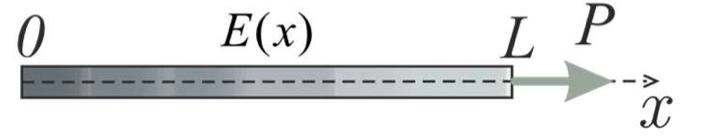
\includegraphics[width=0.3\textwidth]{images/19.1.jpg}

$x \in(0 ; L), \varepsilon(x) \equiv \varepsilon=\langle\varepsilon\rangle_x$
$\sigma(x)=E(x) \varepsilon \Rightarrow\langle\sigma(x)\rangle_x=\langle E(x) \varepsilon\rangle_x=\langle E(x)\rangle_x \varepsilon=\langle E(x)\rangle_x\langle\varepsilon\rangle_x \Rightarrow E_x^F=\langle E(x)\rangle_x \equiv \frac{1}{L} \int_0^L E(x) d x $

\textbf{Эффективный модуль Фойхта} можно приближенно определить из решения 3D краевой задачи на одноосное растяжение неоднородного стержня, когда нагруженная грань остаётся плоской и перпендикулярной оси стержня. Рассмотрим градиентный по ширине прямоугольный стержень, такой, что коэффициент Пуассона меняются мало: $\left|v^{\prime}(x)\right| \ll 1$. Пусть $u_3=\varepsilon z$, $, u_1=-v \varepsilon x, u_2=-v \varepsilon y, \varepsilon=$ const - относительное удлинение стержня. Условия Сен-Венана выполнены тождественно. Убедимся, что тензор деформаций является приближенно постоянным и оси $O X Y Z$ - главные:

\begin{figure}[h!]
  \centering
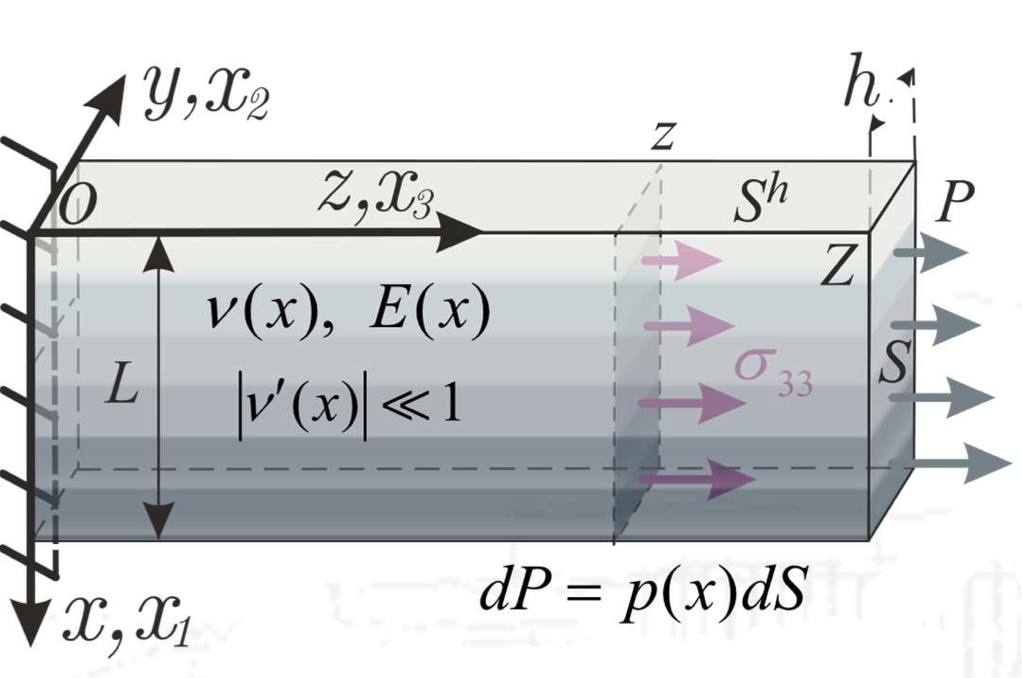
\includegraphics[width=0.4\textwidth]{images/19.2.jpg}
\end{figure}



$
\varepsilon_{33}=u_{3,3}=\varepsilon,\quad
\varepsilon_{11}=u_{1,1}=-v^{\prime}(\varepsilon x)-v \varepsilon \approx-v \varepsilon,\quad \varepsilon_{22}=u_{2,2}=-v \varepsilon,\quad
2 \varepsilon_{12}=u_{1,2}+u_{2,1}=u_{2,1}=-v^{\prime} \varepsilon y \approx 0, \varepsilon_{13}=\varepsilon_{23}=0 \\
\sigma_{i j}=\lambda(x) \theta \delta_{i j}+2 \mu(x) \varepsilon_{i j} \Rightarrow \sigma_{33}=\lambda \theta+2 \mu \varepsilon_{33}=(\lambda(1-2 v)+2 \mu) \varepsilon=E(x) \varepsilon \\
\sigma_{11}=\lambda \theta+2 \mu \varepsilon_{11}=(\lambda(1-2 v)-2 \mu v) \varepsilon=\left(\frac{E v}{1+v}-\frac{E v}{1+v}\right) \varepsilon=0=\sigma_{22}=\sigma_{12}=\sigma_{13}=\sigma_{23}
$
($\triangle Z / Z=u_3(Z) / Z=\varepsilon=\left\langle\varepsilon_{33}\right\rangle$ )


Уравнение равновесия:

$
\sigma_{i j, 1}=0 \Rightarrow \sigma_{11,1}+\sigma_{12,2}+\sigma_{13,3}=0, \sigma_{21,1}+\sigma_{22,2}+\sigma_{23,3}=0, \sigma_{31,1}+\sigma_{32,2}+\sigma_{33,3}=0
$

Среднее по объему третьей компоненты напряжения: 

$\sigma_{33,3}=0 \Rightarrow\left\langle\sigma_{33}\right\rangle=\frac{1}{V} \int_{V} \sigma_{33} d V=\frac{1}{V} \int_{0}^{Z} d z \int_{S} \sigma_{33} d S=\frac{Z}{V} \int_{S} \sigma_{33} d S=\frac{1}{S} \int_{S} p d S=\frac{P}{S}$

Расчетное и экспериментальное определения эффективного модуля Фойхта:

$\left\langle\sigma_{33}\right\rangle=\langle E \varepsilon\rangle=\langle E\rangle \varepsilon^{V}=\langle E\rangle\left\langle\varepsilon_{33}\right\rangle \Rightarrow\langle E(x)\rangle=E^{\mathrm{F}}=\frac{P}{\varepsilon S}$

Кусочно-однородный стержень с сильно различными константами. Считаем, что в каждой из фаз приближенно реализовано состояние равномерного растяжения, так что:

\begin{figure}[h!]
  \centering
  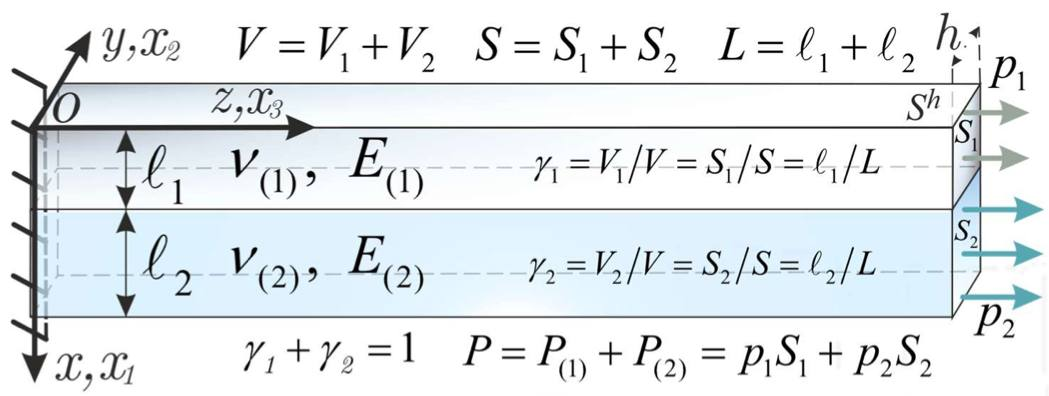
\includegraphics[width=0.5\textwidth]{images/19.3.jpg}
\end{figure}




$\sigma_{i j}(x)=\sigma(x) \delta_{i3} \delta_{j3}, \sigma(x)=\left\{\begin{array}{l}
p_1, x \in\left[0 ; \ell_1\right) \\
p_2, x \in\left(\ell_1 ; L\right]
\end{array}, \frac{p_1}{E_{(1)}}=\varepsilon=\frac{p_2}{E_{(2)}}\right. (x=l_1)$



$
\displaystyle
    \frac{P}{S}=\frac{P_{(1)}}{S}+\frac{P_{(2)}}{S}=\frac{S_1}{S} \frac{P_{(1)}}{S_1}+\frac{S_2}{S} \frac{P_{(2)}}{S_2}=\gamma_1 P_1+\gamma_2 P_2=\gamma_1 E_{(1)} \frac{p_1}{E_{(1)}}+\gamma_2 E_{(2)} \frac{p_2}{E_{(2)}}=\left(\gamma_1 E_{(1)}+\gamma_2 E_{(2)}\right) \varepsilon\Rightarrow\gamma_1 E_{(1)}+\gamma_2 E_{(2)}=\frac{P}{\varepsilon S}
$


$
\displaystyle
    \left\langle\sigma_{33}\right\rangle=\frac{1}{V} \int \limits_{V} \sigma(x) d V=\frac{1}{V} \int \limits_{V_1} p_1 d V+\frac{1}{V} \int_{V_2} p_2 d V=\frac{V_1}{V} p_1+\frac{V_2}{V} p_2=\gamma_1 p_1+\gamma_2 p_2 
$


$
\displaystyle
    \Rightarrow\langle\sigma_{33}\rangle=\frac{P}{S} \Rightarrow E^F\equiv\frac{\langle\sigma_{33}\rangle}{\varepsilon}=\frac{PS}{\varepsilon S}=\gamma_1 E_{(1)}+\gamma_2 E_{(2)} \
$

$
\displaystyle
\varepsilon_{33}^{(1)}=\varepsilon_{33}^{(2)}=\ldots=\varepsilon_{33}^{(N)}=\varepsilon,
\left\langle\sigma_{33}\right\rangle=\sum_{i=1}^{N} \gamma_{i} p_{i}=\frac{P}{S}, 
$


\textbf{Прямая формула смесей:} 
$
\sum_{i=1}^{N} \gamma_{i} E_{(i)}=E^{\mathrm{F}}=\frac{Z \cdot P}{\Delta Z \cdot S}$

\section{Эффективные определяющие соотношения. Эффективный модуль Рейсса. Обратная формула смесей.}
- \textbf{Определяющие соотношения} - это соотношения между причинами и следствиями процессов, которые происходят в телах. Примеры: уравнение Менделеева-Клайперона; закон Гука; закон Навье-Стокса.

- \textbf{Эффективные определяющие соотношения} - это соотношения, связывающие между собой средние по представительному объёму значения причин и следствий. Материальные константы и материальные функции, входящие в эти соотношения, называются эффективными физико-механическими свойствами (характеристиками) композита.

- Экспериментальное определение всего комплекса эффективных свойств композита является дорогим и долгим процессом. Поэтому необходимы математические методы вычисления эффективных характеристик, позволяющие с разной степенью точности вычислять эффективные свойства.

- В МДТТ под эффективными определяющими соотношениями понимаются соотношения позволяющие выразить средние напряжения через средние деформации ($\langle\underset{\sim}{\boldsymbol{\sigma}}\rangle \sim\langle\underset{\sim}{\boldsymbol{\varepsilon}}\rangle$ - это прямые соотношения), либо наоборот средние деформации через средние напряжения ( $\langle\underset{\sim}{\boldsymbol{\varepsilon}}\rangle \sim\langle\underset{\sim}{\boldsymbol{\sigma}}\rangle$ - это обратные соотношения).

- Материальные константы и материальные функции, входящие в эти соотношения, называются эффективными константами и соответственно эффективными функциями композита.

- В общем случае эффективные материальные константы и функции, получаемые из прямых и обратных определяющих соотнощений, не являются взаимно обратными, то есть эффективные прямые и обратные соотношения не обязательно совпадают. 

\textbf{Эффективный модуль Рейсса} определим при следующих предположениях: 1) фазы являются изотропными и линейно-упругими; 2) нет массовых сил; 3) тело находится в состоянии статического равновесия; 4) поле напряжений однородно: 

$\sigma_{i j}=$ const. $\Rightarrow\left\langle\varepsilon_{i j}(\vec{x})\right\rangle=\left\langle C_{i j k l}^{-1} \sigma_{k l}\right\rangle=\left\langle C_{i j k l}^{-1}\right\rangle \sigma_{k l}=\left\langle C_{i j k l}^{-1}\right\rangle\left\langle\sigma_{k l}\right\rangle \Rightarrow C_{i j k l}^{\mathrm{R}}=\left\langle C_{i j k l}^{-1}\right\rangle^{-1}$. 
Рассмотрим сначала линейно-упруаий одномерный отрезок: 
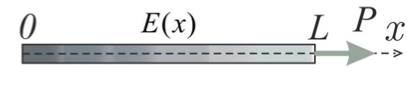
\includegraphics[width=0.3\textwidth]{images/20.1.jpg}

$x \in(0 ; L), \sigma(x) \equiv \sigma=\langle\sigma\rangle$ 
$\displaystyle
\varepsilon(x)=\frac{\sigma}{E(x)} \Rightarrow\langle\varepsilon(x)\rangle_x=\left\langle\frac{1}{E(x)} \sigma\right\rangle_x=\left\langle\frac{1}{E(x)}\right\rangle_x \sigma=\left\langle\frac{1}{E(x)}\right\rangle_x\langle\sigma\rangle_x \Rightarrow E_x^{\mathrm{R}}=\left\langle\frac{1}{E(x)}\right\rangle_x^{-1} \equiv\left\langle\frac{1}{L} \int_0^L \frac{1}{E(x)} d x\right)
$

\vspace{0.5cm}

\textbf{Эффективный модуль Рейсса} можно приближенно определить из решения 3D краевой задачи на одноосное растяжение неоднородного стержня, когда нагруженная грань остаётся плоской и перпендикулярной оси стержня. Рассмотрим градиентный по длине прямоугольный стержень такой, что свойства меняются мало: 

$\left|v^{\prime}(x)\right| \ll 1, \left|E^{\prime}(x)\right| \ll 1$ 

\begin{figure}[h!]
  \centering
  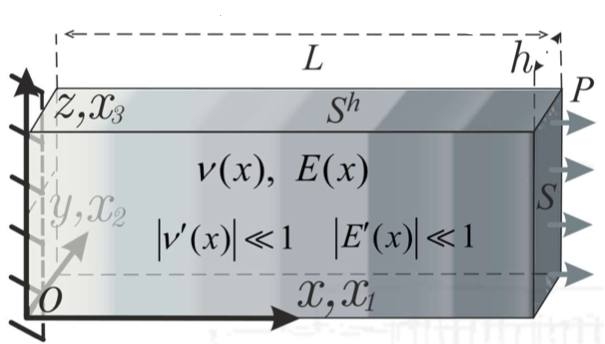
\includegraphics[width=0.4\textwidth]{images/20.2.jpg}
\end{figure}



Предположим, что: $\sigma_{i j}=p \delta_{i 1} \delta_{j 1} \Rightarrow \mathrm{tr} \underset{\mathrm{\sigma }}{\mathrm{\sigma }}=p \Rightarrow \varepsilon_{i j}(x)=-\frac{v(x)}{E(x)} p \delta_{i j}+\frac{1+v(x)}{E(x)} \sigma_{i j}$
$
\varepsilon_{i j}(x)=\frac{p}{E(x)}\left(-v(x) \delta_{i j}+(1+v(x)) \delta_{i 1} \delta_{j 1}\right) \Rightarrow \varepsilon_{22}(x)=\varepsilon_{33}(x)=\frac{-v(x)}{E(x)} p, \varepsilon_{11}(x)=\frac{p}{E(x)}, \varepsilon_{12}=\varepsilon_{13}=\varepsilon_{23}=0
$


Уравнения совместности Сен-Венана: $\quad \varepsilon_{11,22}+\varepsilon_{22,11}=2 \varepsilon_{12,12} \Rightarrow \varepsilon_{22,11}=0 \quad$ 
$\quad\left(\frac{-v(x)}{E(x)} p\right)_{,11} \approx 0${\Large (?)}
Предложенное решение является приближенным. (Уравнения равновесия, краевые условия и четыре ур-ия Сен-Венана выполнены точно. Два ур-ия выполнены приближенно.)


Средняя по объему
продольная деформация:
$$
\varepsilon_{11,2}=\varepsilon_{11,3}=0 \Rightarrow\left\langle\varepsilon_{11}\right\rangle=\frac{1}{V} \int_V \varepsilon_{11} d V=\frac{1}{V} \int_S d S \int_0^L \varepsilon_{11} d x=\frac{S}{V} \int_0^L \varepsilon_{11} d x=\frac{\Delta L}{L}
$$
Расчетное и экспериментальное определения эффективного модуля Рейсса

$
\left\langle\varepsilon_{11}\right\rangle=\left\langle\frac{p}{E}\right\rangle=\left\langle\frac{1}{E}\right\rangle p=\left\langle\frac{1}{E}\right\rangle\left\langle\sigma_{11}\right\rangle \Rightarrow\left\langle\frac{1}{E(x)}\right\rangle^{-1}=E^{\mathrm{R}}=\frac{p L}{\Delta L} 
$

Кусочно-однородный стержень с сильно различными константами. Считаем, что в каждой из фаз приближенно реализовано состояние равномерного растяжения, так что:


\begin{figure}[h!]
  \centering
  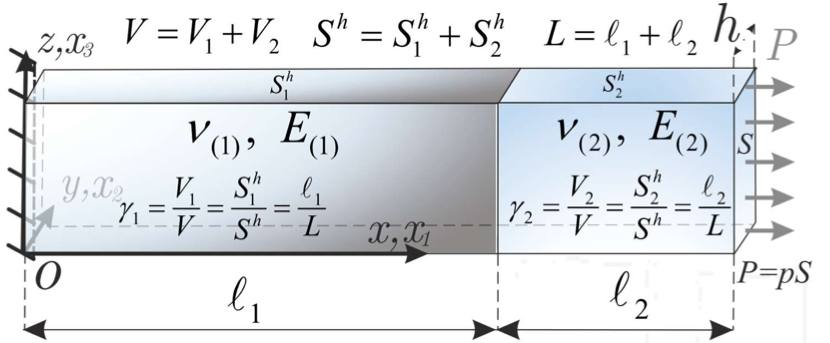
\includegraphics[width=0.6\textwidth]{images/20.3.jpg}
\end{figure}



$\displaystyle
\sigma_{i j}=p \delta_{i 1} \delta_{j 1}, \varepsilon_{11}(x)=\left\{\begin{array}{l}
\varepsilon_{(1)}, x \in\left[0 ; \ell_1\right) \\
\varepsilon_{(2)}, x \in\left(\ell_1 ; L\right]
\end{array}, E_{(1)} \varepsilon_{(1)}=p=E_{(2)} \varepsilon_{(2)}\right.$

$\displaystyle
\frac{\Delta L}{L}=\frac{\Delta \ell_1}{L}+\frac{\Delta \ell_2}{L}=\frac{\ell_1}{L} \frac{\Delta \ell_1}{\ell_1}+\frac{\ell_2}{L} \frac{\Delta \ell_2}{\ell_2}= \gamma_1 \varepsilon_{(1)}+\gamma_2 \varepsilon_{(2)}=\frac{\gamma_1}{E_{(1)}} E_{(1)} \varepsilon_{(1)}+\frac{\gamma_2}{E_{(2)}} E_{(2)} \varepsilon_{(2)}=\left(\frac{\gamma_1}{E_{(1)}}+\frac{\gamma_2}{E_{(2)}}\right) p \Rightarrow \frac{\gamma_1}{E_{(1)}}+\frac{\gamma_2}{E_{(2)}}=\frac{\Delta L}{p L} $

$\displaystyle
\left\langle\varepsilon_{11}\right\rangle=\frac{1}{V} \iint_V \varepsilon(x) d V=\frac{1}{V} \int_{V_1} \varepsilon_{(1)} d V+\frac{1}{V} \int_{V_2} \varepsilon_{(2)} d V=\frac{V_1}{V} \varepsilon_{(1)}+\frac{V_2}{V} \varepsilon_{(2)}=\gamma_1 \varepsilon_{(1)}+\gamma_2 \varepsilon_{(2)} \Rightarrow\left\langle\varepsilon_{11}\right\rangle=\frac{\Delta L}{L} \Rightarrow \frac{1}{E^{\mathrm{R}}} \equiv \frac{\left\langle\varepsilon_{11}\right\rangle}{p}=\frac{\Delta L}{p L}=\frac{\gamma_1}{E_{(1)}}+\frac{\gamma_2}{E_{(2)}}$
 

 
$
\displaystyle
\sigma_{11}^{(1)}=\sigma_{11}^{(2)}=\ldots=\sigma_{11}^{(N)}=p,\left\langle\varepsilon_{11}\right\rangle=\sum_{i=1}^N \gamma_i \varepsilon_{(i)}, 
$


\textbf{Обратная формула смесей:}
$\sum_{i=1}^N \frac{\gamma_i}{E_{(i)}}=\frac{1}{E^{\mathrm{R}}}=\frac{S \cdot \Delta L}{P \cdot L}$


\section{Эффективные модули слоисто-волокнистого композита в плоско-напряженном состоянии в главных осях. Формула Акасаки для эффективного трансверсального модуля.}

\begin{figure}[h!]
  \centering
  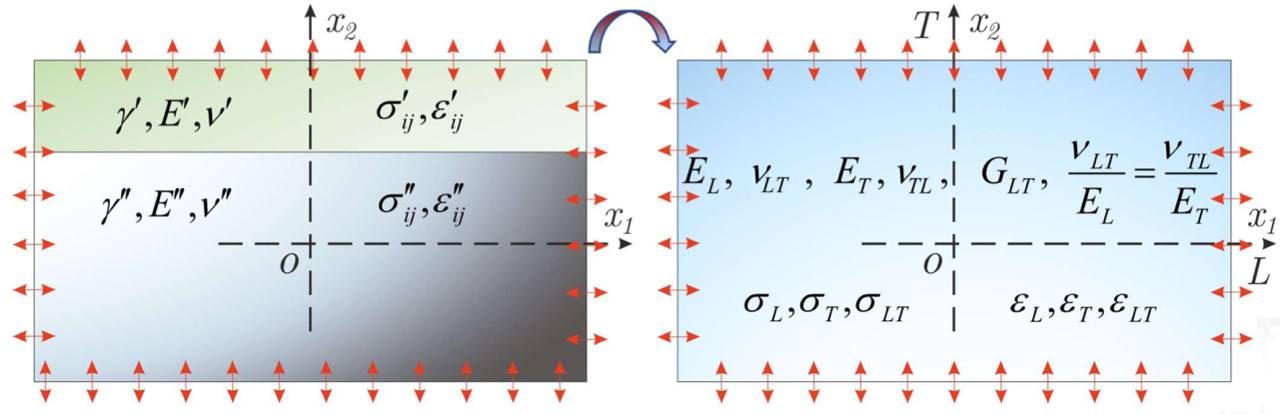
\includegraphics[width=0.9\textwidth]{images/21.1.jpg}
\end{figure}

$$
\left(\sigma_L, \sigma_T, \sigma_{L T}\right)=\left(\sigma_{11}, \sigma_{22}, \sigma_{12}\right) ;\left(\varepsilon_L, \varepsilon_T, \varepsilon_{L T}\right)=\left(\varepsilon_{11}, \varepsilon_{22}, 2 \varepsilon_{12}\right)
$$

Эффективные плоские модули определим при следующих предположениях: 1) фазы являются линейно-упругими и изотропными; 2) нет массовых сил; 3) тело находится в состоянии статического равновесия; 4) состояние является плоско-напряженным и главные оси тензора напряжений сонаправлены со сторонами пластины.


($E_L$ эффективный продольный модуль Юнга, $E_T$ эффективный поперечный модуль Юнга)

При указанных условиях проверим гипотезу, что модель композита является ортотропной с главными осями \textit{LT}.

$
\displaystyle
\left(\begin{array}{l}
\varepsilon_1^{\prime} \\
\varepsilon_2^{\prime} \\
\varepsilon_6^{\prime}
\end{array}\right)=\left(\begin{array}{ccc}
1 / E^{\prime} & -v^{\prime} / E^{\prime} & 0 \\
-v^{\prime} / E^{\prime} & 1 / E^{\prime} & 0 \\
0 & 0 & 1 / G^{\prime}
\end{array}\right)\left(\begin{array}{l}
\sigma_1^{\prime} \\
\sigma_1^{\prime} \\
\sigma_6^{\prime}
\end{array}\right),
\left(\begin{array}{l}
\varepsilon_1^{\prime \prime} \\
\varepsilon_2^{\prime \prime} \\
\varepsilon_6^{\prime \prime}
\end{array}\right)=\left(\begin{array}{ccc}
1 / E^{\prime \prime} & -v^{\prime \prime} / E^{\prime \prime} & 0 \\
-v^{\prime \prime} / E^{\prime \prime} & 1 / E^{\prime \prime} & 0 \\
0 & 0 & 1 / G^{\prime \prime}
\end{array}\right)\left(\begin{array}{l}
\sigma_1^{\prime \prime} \\
\sigma_1^{\prime \prime} \\
\sigma_6^{\prime \prime}
\end{array}\right)
\textbf{???} 
\left(\begin{array}{l}
\varepsilon_L \\
\varepsilon_T \\
\varepsilon_{L T}
\end{array}\right)=\left(\begin{array}{ccc}
1 / E_L & -v_{T L} / E_T & 0 \\
-v_{L T} / E_L & 1 / E_T & 0 \\
0 & 0 & 1 / G_{L T}
\end{array}\right)\left(\begin{array}{l}
\sigma_L \\
\sigma_T \\
\sigma_{L T}
\end{array}\right) \textbf{???}$


Примем принцип суперпозиции двух одномерных задач. Это позволит нам определить средние по объёму значения диагональных компонент тензоров напряжений и деформаций. Средние значения совпадают со значениями в модели композита:
$$
\begin{aligned}
& \varepsilon_1^{\prime}=\varepsilon_1^{\prime \prime}=\left\langle\varepsilon_{11}\right\rangle \equiv \varepsilon_L ; \quad \gamma^{\prime} \sigma_1^{\prime}+\gamma^{\prime \prime} \sigma_1^{\prime \prime}=\left\langle\sigma_{11}\right\rangle \equiv \sigma_L \\
& \sigma_2^{\prime}=\sigma_2^{\prime \prime}=\left\langle\sigma_{22}\right\rangle \equiv \sigma_T ; \quad \gamma^{\prime} \varepsilon_2^{\prime}+\gamma^{\prime \prime} \varepsilon_2^{\prime \prime}=\left\langle\varepsilon_{11}\right\rangle \equiv \varepsilon_T
\end{aligned}
$$

Запишем получившуюся систему уравнений. Из этих равенств надо исключить: $\varepsilon_1^{\prime}, \varepsilon_2^{\prime}, \sigma_1^{\prime}, \sigma_2^{\prime}, \varepsilon_1^{\prime \prime}, \varepsilon_2^{\prime \prime}, \sigma_1^{\prime \prime}, \sigma_2^{\prime \prime}$.

$$\left\{\begin{array} { l } 
{ \varepsilon _ { 1 } ^ { \prime } = \varepsilon _ { 1 } ^ { \prime \prime } = \varepsilon _ { L } } \\
{ \gamma ^ { \prime } \sigma _ { 1 } ^ { \prime } + \gamma ^ { \prime \prime } \sigma _ { 1 } ^ { \prime \prime } = \sigma _ { L } } \\
{ \sigma _ { 2 } ^ { \prime } = \sigma _ { 2 } ^ { \prime \prime } = \sigma _ { T } } \\
{ \gamma ^ { \prime } \varepsilon _ { 2 } ^ { \prime } + \gamma ^ { \prime \prime } \varepsilon _ { 2 } ^ { \prime \prime } = \varepsilon _ { T } }
\end{array} \left\{\begin{array}{l}
E^{\prime} \varepsilon_1^{\prime}=\sigma_1^{\prime}-v^{\prime} \sigma_2^{\prime} \\
E^{\prime} \varepsilon_2^{\prime}=\sigma_2^{\prime}-v^{\prime} \sigma_1^{\prime} \\
E^{\prime \prime} \varepsilon_1^{\prime \prime}=\sigma_1^{\prime \prime}-v^{\prime \prime} \sigma_2^{\prime \prime} \\
E^{\prime \prime} \varepsilon_2^{\prime \prime}=\sigma_2^{\prime \prime}-v^{\prime \prime} \sigma_1^{\prime \prime}
\end{array}\right.\right.$$

$$
\left\{\begin{array}{l}
E^{\prime} \varepsilon_L=\sigma_1^{\prime}-v^{\prime} \sigma_T \mid \cdot \gamma^{\prime} \\
E^{\prime \prime} \varepsilon_L=\sigma_1^{\prime \prime}-v^{\prime \prime} \sigma_T \mid \cdot \gamma^{\prime \prime}
\end{array}\right. \Rightarrow$$

$$\left(\gamma^{\prime} E^{\prime}+\gamma^{\prime \prime} E^{\prime \prime}\right) \varepsilon_L \stackrel{{\gamma}^{\prime} \sigma_1^{\prime}+\gamma^{\prime \prime} \sigma_{1}^{\prime \prime}=\sigma_L}{=}
\quad \underbrace{\left(\gamma^{\prime} \sigma_1^{\prime}+\gamma^{\prime \prime} \sigma_1^{\prime \prime}\right)}\limits_{\sigma_L}-\left(\gamma^{\prime} v^{\prime}+\gamma^{\prime \prime} v^{\prime \prime}\right) \sigma_T \Rightarrow
$$
$$
\varepsilon_L=\frac{1}{\gamma^{\prime} E^{\prime}+\gamma^{\prime \prime} E^{\prime \prime}} \sigma_L-\frac{\gamma^{\prime} v^{\prime}+\gamma^{\prime \prime} v^{\prime \prime}}{\gamma^{\prime} E^{\prime}+\gamma^{\prime \prime} E^{\prime \prime}} \sigma_T \quad \Rightarrow \quad E_L=\gamma^{\prime} E^{\prime}+\gamma^{\prime \prime} E^{\prime \prime}, \quad \frac{v_{T L}}{E_T}=\frac{\gamma^{\prime} v^{\prime}+\gamma^{\prime \prime} v^{\prime \prime}}{\gamma^{\prime} E^{\prime}+\gamma^{\prime \prime} E^{\prime \prime}}
$$
$$
\left\{\begin{array}{l}
\varepsilon_2^{\prime}=1 / E^{\prime}\left(\sigma_T-v^{\prime} \sigma_1^{\prime}\right) \mid \cdot \gamma^{\prime} \\
\varepsilon_2^{\prime \prime}=1 / E^{\prime \prime}\left(\sigma_T-v^{\prime \prime} \sigma_1^{\prime \prime}\right) \mid \cdot \gamma^{\prime \prime}
\end{array}\right.$$
$$
\varepsilon_T=\left(\frac{\gamma^{\prime}}{E^{\prime}}+\frac{\gamma^{\prime \prime}}{E^{\prime \prime}}\right) \sigma_T-\frac{\gamma^{\prime} v^{\prime}}{E^{\prime}} \underbrace{\left(E^{\prime} \varepsilon_L+v^{\prime} \sigma_T\right)}_{\sigma_1^{\prime}}-\frac{\gamma^{\prime \prime} v^{\prime \prime}}{E^{\prime \prime}} \underbrace{\left(E^{\prime \prime} \varepsilon_L+v^{\prime \prime} \sigma_T\right)}_{\sigma_1^{\prime\prime}}
$$
$$
\begin{aligned}
& \varepsilon_T=\left(\frac{\gamma^{\prime}}{E^{\prime}}+\frac{\gamma^{\prime \prime}}{E^{\prime \prime}}-\frac{\gamma^{\prime}\left(v^{\prime}\right)^2}{E^{\prime}}-\frac{\gamma^{\prime \prime}\left(v^{\prime \prime}\right)^2}{E^{\prime \prime}}\right) \sigma_T-\left(\gamma^{\prime} v^{\prime}+\gamma^{\prime \prime} v^{\prime \prime}\right) \underbrace{\left(\frac{\sigma_L}{E_L}-\frac{\gamma^{\prime} v^{\prime}+\gamma^{\prime \prime} v^{\prime \prime}}{E_L} \sigma_T\right)} \limits_{\varepsilon_L} \\
\end{aligned}
$$
$$
\varepsilon_T=-\frac{\overbrace{\gamma^{\prime} v^{\prime}+\gamma^{\prime \prime} v^{\prime \prime}}^{v_{L T}}}{E_L} \sigma_L+\left(\frac{\gamma^{\prime}}{E^{\prime}}+\frac{\gamma^{\prime \prime}}{E^{\prime \prime}}-\frac{\gamma^{\prime}\left(v^{\prime}\right)^2}{E^{\prime}}-\frac{\gamma^{\prime \prime}\left(v^{\prime \prime}\right)^2}{E^{\prime \prime}}+\frac{\left(\gamma^{\prime} v^{\prime}+\gamma^{\prime \prime} v^{\prime \prime}\right)^2}{\underbrace{\gamma^{\prime} E^{\prime}+\gamma^{\prime \prime} E^{\prime \prime}}_{E_L}}\right) \sigma_T 
$$
$$
\Rightarrow 
(\varepsilon_T=-\frac{v_{LT}}{E_L}\sigma_L+\frac{1}{E_T}\sigma_T) \Rightarrow
$$
$$
\displaystyle
\begin{aligned}
& \frac{1}{E_T}=\left(\frac{\gamma^{\prime}}{E^{\prime}}+\frac{\gamma^{\prime \prime}}{E^{\prime \prime}}\right)-\frac{\gamma^{\prime}\left(v^{\prime}\right)^2}{E^{\prime}}-\frac{\gamma^{\prime \prime}\left(v^{\prime \prime}\right)^2}{E^{\prime \prime}}+\frac{\left(\gamma^{\prime} v^{\prime}+\gamma^{\prime \prime} v^{\prime \prime}\right)^2}{\gamma^{\prime} E^{\prime}+\gamma^{\prime \prime} E^{\prime \prime}}=\left(\frac{\gamma^{\prime}}{E^{\prime}}+\frac{\gamma^{\prime \prime}}{E^{\prime \prime}}\right)-\frac{*}{E^{\prime} E^{\prime \prime} E_L} \Rightarrow \\
& *=\gamma^{\prime}\left(v^{\prime}\right)^2 E^{\prime \prime}\left(\underline{\gamma^{\prime} E^{\prime}}+\gamma^{\prime \prime} E^{\prime \prime}\right)+\gamma^{\prime \prime}\left(v^{\prime \prime}\right)^2 E^{\prime}\left(\gamma^{\prime} E^{\prime}+\underline{\gamma^{\prime \prime} E^{\prime \prime}}\right)-\underline{E^{\prime} E^{\prime \prime}\left(\gamma^{\prime} v^{\prime}+\gamma^{\prime \prime} v^{\prime \prime}\right)^2}= \\
& \left(\left(\gamma^{\prime} v^{\prime}\right)^2+\left(\gamma^{\prime \prime} v^{\prime \prime}\right)^2-\left(\gamma^{\prime} v^{\prime}+\gamma^{\prime \prime} v^{\prime \prime}\right)^2\right) E^{\prime} E^{\prime \prime}+\gamma^{\prime} \gamma^{\prime \prime}\left(\left(v^{\prime} E^{\prime \prime}\right)^2+\left(v^{\prime \prime} E^{\prime}\right)^2\right)=-2 \gamma^{\prime} v^{\prime} \gamma^{\prime \prime} v^{\prime \prime} E^{\prime} E^{\prime \prime}+ \\
& +\gamma^{\prime} \gamma^{\prime \prime}\left(\left(v^{\prime} E^{\prime \prime}\right)^2+\left(v^{\prime \prime} E^{\prime}\right)^2\right)=\gamma^{\prime} \gamma^{\prime \prime}\left(v^{\prime} E^{\prime \prime}-v^{\prime \prime} E^{\prime}\right)^2 \Rightarrow 
\\& \textbf{Формула Акасаки:} \frac{1}{E_T}=\left(\frac{\gamma^{\prime}}{E^{\prime}}+\frac{\gamma^{\prime \prime}}{E^{\prime \prime}}\right)-\gamma^{\prime} \gamma^{\prime \prime} \frac{\left(v^{\prime} / E^{\prime}-v^{\prime \prime} / E^{\prime \prime}\right)^2}{\gamma^{\prime} / E^{\prime \prime}+\gamma^{\prime \prime} / E^{\prime}} \\
& v_{L T}=\gamma^{\prime} v^{\prime}+\gamma^{\prime \prime} v^{\prime \prime} ; \quad E_L=\gamma^{\prime} E^{\prime}+\gamma^{\prime \prime} E^{\prime \prime} ; \quad v_{T L}=\frac{E_T}{E_L} v_{L T} ; \quad \\& \frac{1}{G_{L T}}=\frac{\gamma^{\prime}}{G^{\prime}}+\frac{\gamma^{\prime \prime}}{G^{\prime \prime}} \Leftarrow \sigma_{12}^{\prime}=\sigma_{12}^{\prime \prime}=\sigma_{L T} \\
&
\end{aligned}
$$



\end{document}